\documentclass[a4paper, 12pt]{scrbook}

\usepackage{math-book}

\begin{document}

\frontmatter


\mainChapter{Vektoranalízis}\label{chap-01}

\bgroup
\color{gray!50!black}
\sffamily

% Lorem ipsum

\chaptertoc
\egroup

\clearpage
\chapter{Jelölések}

\begin{blueBox}
  Ez egy egyszerű szövegdoboz.
\end{blueBox}

\begin{note}
  Ez egy megjegyzés.
\end{note}

\begin{statement}
  Ez egy állítás.
\end{statement}

\begin{example}
  Ez egy példa.
\end{example}

\begin{learnMore}
  Ez egy kitekintés.
\end{learnMore}

\begin{definition}
  Ez egy definíció.
\end{definition}

\begin{theorem}
  Ez egy tétel.
\end{theorem}

\begin{mdframed}[style=questions, frametitle={\color{white}Felkészülést segítő kérdések}]
  Ezek segítenek a tanulásban.
\end{mdframed}

% \newcommand{\tname}[1]{\marginnote{\sffamily\bfseries\color{primaryColor}#1}}
\newcommand{\mfrac}[2]{\frac{{#1}^{\mathstrut}}{{#2}_{\mathstrut}}}
\newcommand{\mwrap}[1]{{#1}^{\mathstrut}_{\mathstrut}}
\newenvironment{notations}[1]{%
  \checkoddpage%
  \ifoddpage%
    % \def\tcbleft{0pt}%
    % \def\tcbright{2pt}%
    \newcolumntype{U}{r<{\hspace{2mm}}}
  \else%
    % \def\tcbleft{2pt}%
    % \def\tcbright{0pt}%
    \newcolumntype{U}{l}
  \fi%
  % \begin{tcolorbox}[
  %     frame hidden,
  %     colframe=white,
  %     boxsep=0pt,
  %     left=0pt,
  %     right=0pt,
  %     top=12mm,
  %     bottom=0pt,
  %     arc=0pt,
  %     outer arc=0pt,
  %   ]
  \begin{center}
    \def\arraystretch{1.55}
    \setlength\arrayrulewidth{1pt}
    \arrayrulecolor{primaryColor}
    \begin{tabular}
      {
      |
      >{\centering\arraybackslash$\displaystyle}m{3.5cm}<{$}
      |
      >{\centering\arraybackslash}m{5cm}
      |
      >{\centering\arraybackslash$\displaystyle}m{6cm}<{$}
      |
      }
      \hline
      \multicolumn{3}{|U|}{
        \sffamily\Large\bfseries\color{white}\cellcolor{primaryColor}
        #1
      }
      \\
      \hline
      \cellcolor{gray!25}\text{\sffamily\color{primaryColor}\textbf{Jel}}
       & \cellcolor{gray!25}\text{\sffamily\color{primaryColor}\textbf{Megnevezés}}
       & \cellcolor{gray!25}\text{\sffamily\color{primaryColor}\textbf{Példa}}
      \\
      \hline
      }{%
      \\
      \hline
    \end{tabular}
  \end{center}
  % \end{tcolorbox}
}

\clearpage

\begin{notations}{Logikai szimbólumok}
  \land       & és               & p \land q
  \\\hline
  \lor        & vagy             & p \lor q
  \\\hline
  \forall     & minden / bármely & \forall x \in X
  \\\hline
  \exists     & létezik          & \exists x \in X
  \\\hline
  % \exists!    & biztosan létezik & \exists! x \in X
  % \\\hline
  \not\exists & nem létezik      & \not\exists x \in X
  % \\\hline
  % !           & legyen           & !x \in X
\end{notations}
\hfill
\begin{notations}{Egyenlőség, relációk}
  =      & egyenlő              & 2 + 2 = 4
  \\\hline
  \neq   & nem egyenlő          & 2 \neq 3
  \\\hline
  \equiv & ekvivalens           & 2 \equiv 2
  \\\hline
  <      & kisebb               & 2 < 3
  \\\hline
  \leq   & kisebb vagy egyenlő  & 2 \leq 3
  \\\hline
  >      & nagyobb              & 3 > 2
  \\\hline
  \geq   & nagyobb vagy egyenlő & 3 \geq 2
\end{notations}
\hfill
\begin{notations}{Műveletek}
  a + b       & összeg        & 2 + 3 = 5
  \\\hline
  a - b       & különbség     & 5 - 3 = 2
  \\\hline
  a \cdot b   & szorzat       & 2 \cdot 3 = 6
  \\\hline
  a / b       & hányados      & 6 / 3 = 2
  \\\hline
  a^b         & hatvány       & 2^3 = 8
  \\\hline
  \sqrt{a}    & négyzetgyök   & \sqrt{4} = 2
  \\\hline
  \sqrt[n]{a} & $n$-edik gyök & \sqrt[3]{8} = 2
  \\\hline
  a!          & faktoriális   & 3! = 3 \cdot 2 \cdot 1 = 6
\end{notations}

\clearpage

\begin{notations}{Halmazok és halmazműveletek}
  \emptyset, \{\} & üreshalmaz
                  & A := \{ k \mid k \in \mathbb N \land k < 0 \}
  \\\hline
  \mathbb N       & természetes számok halmaza
                  & 1, 2, 3, \dots
  \\\hline
  \mathbb Z       & egész számok halmaza
                  & \dots, -2, -1, 0, 1, 2, \dots
  \\\hline
  \mathbb Q       & racionális számok halmaza
                  & 2/3 \in \mathbb{Q}
  \\\hline
  \mathbb Q^*     & irracionális számok halmaza
                  & \pi \in \mathbb{Q}
  \\\hline
  \mathbb R       & valós számok halmaza
                  & \sqrt{2} \in \mathbb{R}
  \\\hline
  \mathbb C       & komplex számok halmaza
                  & i \in \mathbb{C}
  \\\hline
  A, B, C         & halmazok
                  & A = \{1; 2; 3\}
  \\\hline
  a, b, c         & halmazok elemei
                  & x \in A
  \\\hline
  \in             & eleme
                  & \iu \in \mathbb C
  \\\hline
  \notin          & nem eleme
                  & \pi \notin \mathbb Q
  \\\hline
  \sim            & ekvivalencia
                  & A \sim B
  \\\hline
  \subseteq       & részhalmaza
                  & \{1\} \subseteq \{1; 2\}
  \\\hline
  \subset         & valódi részhalmaza
                  & A \subset B \Leftrightarrow A \subseteq B \land A \neq B
  \\\hline
  \overline A     & komplementer halmaz
                  & \{x \in X \mid x \notin A\}
  \\\hline
  \cup            & unió
                  & \{x \in X \mid x \in A \lor x \in B\}
  \\\hline
  \cap            & metszet
                  & \{x \in X \mid x \in A \land x \in B\}
  \\\hline
  \setminus       & kivonás
                  & \{x \in X \mid x \in A \land x \notin B\}
\end{notations}
\hfill
\begin{notations}{Intervallumok}
  [a; b] & zárt intervallum                         & [0; 1]
  \\\hline
  (a; b) & nyílt intervallum                        & (0; 1)
  \\\hline
  [a; b) & balról zárt, jobbról nyitott intervallum & [0; 1)
  \\\hline
  (a; b] & balról nyitott, jobbról zárt intervallum & (0; 1]
\end{notations}

\clearpage

% \begin{notations}{Konstansok}
%   \pi & pi                 & \pi \approx 3.14159
%   \\\hline
%   e   & Euler-féle szám    & e \approx 2.71828
%   \\\hline
%   \iu & imaginárius egység & \iu^2 = -1
% \end{notations}
% \vfill
\begin{notations}{Komplex számok}
  \mathbb C
   & komplex számok halmaza
   & z \in \mathbb C
  \\\hline
  \iu
   & imaginárius egység
   & \iu^2 = -1
  \\\hline
  z
   & komplex szám
   & z = 3 + 4 \iu
  \\\hline
  z = a + b \iu
   & algebrai alak
   & \iRe \{z\} = a, \iIm \{z\} = b
  \\\hline
  \overline z = a - b \iu
   & konjugált
   & \overline{3 + 4\iu} = 3 - 4\iu
  \\\hline
  \iRe \{ z \}
   & valós rész
   & z = 3 + 2\iu \;\rightarrow\; \iRe \{z\} = 3
  \\\hline
  \iIm \{ z \}
   & képzetes rész
   & z = 1 + 4\iu \;\rightarrow\; \iIm \{z\} = 4
  \\\hline
  | z |
   & abszolút érték / hossz
   & | z | = \sqrt{a^2 + b^2}
  \\\hline
  \arg \{z\}
   & argumentum
   & \arg \{z\} = \arctan(b/a)
  \\\hline
  z = r (\cos \varphi + \iu \sin \varphi)
   & trigonometrikus alak
   & | z | = r, \arg \{z\} = \varphi
  \\\hline
  z = r e^{\iu \varphi}
   & exponenciális alak
   & z = r e^{\iu \varphi} = r \exp(\iu \varphi)
\end{notations}
\vfill
\begin{notations}{Sorozatok, sorok}
  (a_n)
   & numerikus sorozat
   & a_n = \mfrac{1}{n}
  \\\hline
  \lim_{n \rightarrow \infty} a_n = a
   & sorozat határértéke
   & \lim_{n \rightarrow \infty} \mfrac{1}{n} = 0
  \\\hline
  a_n = a_{n - 1} + d
   & számtani sorozat
   & a_n = a_{n - 1} + 2
  \\\hline
  a_n = a_{n - 1} \cdot q
   & mértani sorozat
   & a_n = a_{n - 1} \cdot 2
  \\\hline
  \mwrap\sum a_n
   & numerikus sor
   & \mwrap{\sum \frac{1}{n}}
  \\\hline
  L = \sum_{n = 0}^{\infty} a_n
   & sor összege
   & L = \mwrap{\sum_{n = 0}^{\infty}} \frac{1}{n} = \infty
  \\\hline
  \mwrap\sum a \cdot r^n
   & \makecell{geometriai sor                               \\ {(${|r| < 1}$ esetén)}}
   & \mwrap{\sum_{n = 0}^{\infty}} \frac{1}{2^n}
  = \frac{1}{1 - r}
  = \frac{1}{1 - \sfrac{1}{2}}
  = 2
\end{notations}

\clearpage

\begin{notations}{Függvények}
  f: \Domain \rightarrow \Range, x \mapsto y
   & $f$ függvény
   & f: \Reals \rightarrow \Reals, x \mapsto x^2
  \\\hline
  \Domain_f
   & értelmezési tartomány
   & \Domain_f = \Reals
  \\\hline
  \Range_f
   & értékkészlet
   & \Range_f = [0; +\infty)
  \\\hline
  \Domain \rightarrow \Range
   & értékkészlet hozzárendelése az értelmezési tartományhoz
   & f: \Reals \rightarrow \Reals
  \\\hline
  x \mapsto y
   & függvényértékek hozzárendelése az ősképekhez
   & f: x \mapsto x^2
  \\\hline
  f^{-1}
   & inverz függvény
   & \text{ha } f(3) = 5 \text{, akkor } f^{-1}(5) = 3
  \\\hline
  f \circ g
   & összetett függvény
   & f(x) = e^x, g(x) = x^2 : {(f \circ g)(x) = e^{x^2}}
  \\\hline
  \lim_{x \rightarrow a} f(x) = A
   & függvény határértéke
   & \lim_{x \rightarrow 0} \mfrac{\sin x}{x} = 1
  \\\hline
  \lim_{x \rightarrow a^{+}} f(x) = A
   & jobboldali
   & \lim_{x \rightarrow 0^{+}} \mfrac{1}{x} = +\infty
  \\\hline
  \lim_{x \rightarrow a^{-}} f(x) = A
   & baloldali
   & \lim_{x \rightarrow 0^{-}} \mfrac{1}{x} = -\infty
\end{notations}
\vfill
\begin{notations}{Nevezetes függvények}
  e^x, \exp x
   & exponenciális függvény
   & x \mapsto e^x
  \\\hline
  \ln x
   & természetes alapú logaritmus
   & x \mapsto \ln x
  \\\hline
  a^x
   & hatványfüggvény
   & x \mapsto 2^x
  \\\hline
  \log_a x
   & $a$ alapú logaritmus
   & x \mapsto \log_2 x
  \\\hline
  % \lg x
  %  & tízes alapú logaritmus
  %  & \lg 100 = 2
  % \\\hline
  \makecell{\sin, \cos,             \\ \tan, \cot}
   & szögfüggvények
   & x \mapsto \sin x
  \\\hline
  \makecell{\arcsin, \arccos,       \\ \arctan, \arccot}
   & inverz szögfüggvények
   & x \mapsto \arcsin x
  \\\hline
  \makecell{\sinh, \cosh,           \\ \tanh, \coth}
   & hiperbolikus függvények
   & x \mapsto \sinh x
  \\\hline
  \makecell{\arcsinh, \arccosh,     \\ \arctanh, \arccoth}
   & inverz hiperbolikus függvények
   & x \mapsto \arcsinh x
\end{notations}

\clearpage

\begin{notations}{Kalkulus}
  f'(x), f''(x), f^{(n)}(x)
   & első, második és $n$-edik derivált (Lagrange-féle jelölés)
   & f'(x) = \lim_{h \to 0} \frac{f(x + h) - f(x)}{h}
  \\\hline
  \odv{f}{x}, \odv[order=2]{f}{x}, \odv[order=n]{f}{x}
   & első, második és $n$-edik derivált (Leibniz-féle jelölés)
   & f'(x) = \odv{f}{x}
  \\\hline
  \dot f, \ddot f, \overset{n}{\dot f}
   & első, második és $n$-edik derivált (Newton-féle jelölés)
   & \dot f = \odv{f}{t}
  \\\hline
  \mwrap{\int_a^b} f(x) \dd x
   & Riemann-integrál
   & \mwrap{\int_0^1} x^2 \dd x = \frac{1}{3}
  \\\hline
  \mwrap{\int} f(x) \dd x
   & határozatlan integrál
   & \mwrap{\int} f(x) \dd x = F(x) + C
  \\\hline
  F
   & $f$ primitív függvénye
   & F'(x) = f(x)
  \\\hline
  f \in \mathcal R [a; b]
   & $f$ Riemann-integrálható az $[a; b]$ intervallumon
   & x^2 \in \mathcal R (-\infty; +\infty)
\end{notations}

\mainmatter


\mainChapter{Vektoranalízis}\label{chap-01}

\bgroup
\color{gray!50!black}
\sffamily

% Lorem ipsum

\chaptertoc
\egroup

\clearpage
\clearpage

\section{Alapfogalmak}\label{sec-01-01}

\begin{definition}[Csoport]
  Legyen G nemüres halmaz, és $\circ$ egy művelet. Ekkor a $(G; \circ)$ csoport,
  ha teljesülnek az alábbiak:
  \begin{enumerate}
    \item $\forall a; b; c \in G: (a \circ b) \circ c = a \circ (b \circ c)$,
          \hfill (\textbf{asszociativitás})

    \item $\exists e \in G: \forall a \in G: e \circ a = a \circ e = a$,
          \hfill(\textbf{egységelem})

    \item $\forall a \in G: \exists a^{-1} \in G:
            a \circ a^{-1} = a^{-1} \circ a = e$.
          \hfill (\textbf{inverzelem})
  \end{enumerate}
\end{definition}

\begin{note}
  Ha a $\circ$ művelet kommutatív, azaz $\forall a, b \in G: a \circ b = b \circ
    a$, akkor a csoportot \textbf{Abel-csoport}nak nevezzük.
\end{note}

\begin{example}
  A $(\mathbb R; \cdot)$, $(\mathbb Q; +)$, $\mathbb C; +$ mindegyike
  Abel-csoport.

  Nem csoport $(\mathbb N; +)$, hiszen nincs inverz elem.

  $(\mathbb Q^*; +)$ sem csoport, mert nem létezik egységelem.
\end{example}

\begin{definition}[Gyűrű]
  Legyen $R$ nemüres halmaz, és $\circ, +$ két művelet. Ekkor a $(R; +, \circ)$
  gyűrű, ha teljesülnek az alábbiak:
  \begin{enumerate}
    \item $(R; +)$ \textbf{Abel-csoport},

    \item $\forall a; b; c \in R: (a \circ b) \circ c = a \circ (b \circ c)$
          \hfill (\textbf{asszociativitás})

    \item teljesül a disztributivitás:
          \begin{itemize}
            \item $\forall a; b; c \in R:
                    a \circ (b + c) = a \circ b + a \circ c$,
                  \hfill (\textbf{$+$ disztributív $\circ$-ra})

            \item $\forall a; b; c \in R:
                    (a + b) \circ c = a \circ c + b \circ c$.
                  \hfill (\textbf{$\circ$ disztributív $+$-ra})
          \end{itemize}
  \end{enumerate}
\end{definition}

\begin{definition}[Test]
  Legyen $T$ nemüres halmaz, és $\circ, +$ két művelet. Ekkor a $(T; +, \circ)$
  test, ha teljesülnek az alábbiak:
  \begin{enumerate}
    \item $(T; +)$ \textbf{Abel-csoport},

    \item $\forall a; b; c \in T: (a \circ b) \circ c = a \circ (b \circ c)$,
          \hfill (\textbf{asszociativitás})

    \item $\exists e \in T: \forall a \in F: e \circ a = a \circ e = a$,
          \hfill (\textbf{egységelem})

    \item $\forall a \in T \exists a^{-1} \in T:
            a \circ a^{-1} = a^{-1} \circ a = e$,
          \hfill (\textbf{inverzelem})

    \item teljesül a \textbf{disztributivitás}.
          % \begin{itemize}
          %   \item $\forall a; b; c \in F: a \circ (b + c) = a \circ b + a \circ c$,
          %         \hfill ($+$ disztributív $\circ$-ra)

          %   \item $\forall a; b; c \in F: (a + b) \circ c = a \circ c + b \circ c$.
          %         \hfill ($\circ$ disztributív $+$-ra)
          % \end{itemize}
  \end{enumerate}
\end{definition}

\begin{example}
  A $(\mathbb R; +, \cdot)$, $(\mathbb Q; +, \cdot)$, $(\mathbb C; +, \cdot)$
  mindegyike test.
\end{example}

\begin{definition}[Vektortér]
  Legyen $V$ nemüres halmaz, és $\circ, +$ két művelet, $T$ test.
  A $(V; +, \circ)$ a $T$ test feletti vektortér, ha teljesülnek az alábbiak:
  \begin{enumerate}
    \item $(V; +)$ Abel-csoport,

    \item $\forall \lambda; \mu \in T \; \land \; \forall \rvec x \in V:
            (\lambda \circ \mu) \circ \rvec x
            = \lambda \circ (\mu \circ \rvec x)$,

    \item ha $\varepsilon$ a $T$-beli egységelem, akkor
          $\forall \rvec x \in V: \varepsilon \circ \rvec x = \rvec x$,

    \item teljesül a disztributivitás:
          \begin{itemize}
            \item $\forall \lambda; \mu \in T \; \land \; \forall \rvec x \in V:
                    \lambda \circ (\rvec x + \rvec y)
                    = \lambda \circ \rvec x + \lambda \circ \rvec y$,

            \item $\forall \lambda; \mu \in T \; \land \; \forall \rvec x \in V:
                    (\lambda + \mu) \circ \rvec x
                    = \lambda \circ \rvec x + \mu \circ \rvec x$.
          \end{itemize}
  \end{enumerate}
\end{definition}

\begin{example}
  A legfeljebb $n$-edfokú polinomok a skalárral való szorzásra és az összeadásra
  vektorteret alkotnak.

  A függvények az összeadásra és a skalárral való szorzásra vektorteret alkotnak.
\end{example}

\begin{definition}[Vektor]
  A vektortér elemeit vektoroknak nevezzük.
  Jelölés: $\rvec x$, vagy $\underbar x$.
\end{definition}

\begin{statement}
  \textbf{A zéruselem és ellentett elem létezése egyértelmű.}

  \begin{proof}
    \begin{enumerate}
      \item {\sffamily A zéruselem létezése egyértelmű}

            Tegyük fel, hogy $\nvec$ és $\hat \nvec$ különböző
            zéruselemek, vagyis $\nvec \neq \hat \nvec$. Ebben az esetben
            $$
              \nvec = \nvec + \hat \nvec = \hat \nvec
              \text.
            $$
            Ez ellentmondás, tehát a zéruselem egyértelmű.

            \bigskip

      \item {\sffamily Az ellentett elem létezése egyértelmű}

            Tegyük fel, hogy $-\rvec v$ és $-\hat{\rvec v}$ egyaránt
            $\rvec v$ ellentettjei, valamint $-\rvec v \neq -\hat{\rvec v}$.
            Ebben az esetben
            $$
              -\hat{\rvec v}
              = (-\rvec v + \rvec v) + (-\hat{\rvec v})
              = (-\rvec v) + (\rvec v + (-\hat{\rvec v}))
              = -\rvec v
              \text.
            $$
            Ez ellentmondás, tehát az ellentett elem egyértelmű.
    \end{enumerate}
  \end{proof}
\end{statement}

\begin{statement}
  0-val való szorzás:
  $\forall \rvec v \in V: 0 \cdot \rvec v = \nvec$.

  \begin{proof}
    \vspace{3em}
  \end{proof}
\end{statement}

\begin{statement}
  Nullvektorral való szorzás:
  $\forall \lambda \in T: \lambda \cdot \nvec = \nvec$.

  \begin{proof}
    \vspace{3em}
  \end{proof}
\end{statement}

\begin{statement}
  $\lambda \cdot \rvec v = \nvec \quad \Longleftrightarrow \quad
    \lambda = 0 \; \lor \; \rvec v = \nvec$

  \begin{proof}
    \vspace{3em}
  \end{proof}
\end{statement}

\begin{definition}[Lineáris függetlenség]

  A $(V; +; \lambda)$ vektortér $\rvec v_1, \rvec v_2, \ldots, \rvec v_n$
  vekrorait lineárisan függetlennek mondjuk, ha a
  $$
    \lambda_1 \rvec v_1
    + \lambda_2 \rvec v_2
    + \ldots
    + \lambda_n \rvec v_n
    = \nvec
  $$
  vektoregyenletnek \textbf{csak a triviális megoldása} létezik, azaz
  $\lambda_1 = \lambda_2 = \ldots = \lambda_n = 0$.

  Ha az egyenletnek nem csak a triviális megoldása létezik, akkor a vektorok
  lineárisan függők.
\end{definition}

\begin{definition}[Altér]
  Legyen $V; +; \lambda$ $\mathbb R$ feletti vektortér, valamint
  $\emptyset \neq L \subset V$. $L$-t altérnek nevezzük a $V$-ben, ha
  $(L; +; \lambda)$ ugyancsak vektortér.
\end{definition}

\begin{example}
  A polinomok vektorterének alterte a legfeljebb $n$-edfokú polinomok
  vektortere.
\end{example}

\begin{statement}
  Alterek metszete ugyancsak altér. Alterek uniója azonban általában nem altér.
\end{statement}

\begin{definition}[Generátorrendszer]
  Legyen $V$ vektortér, valamint $\emptyset \neq G \subset V$. $G$ által
  generált altérnek nevezzük azt a legszűkebb alteret, amely tartalmazza $G$-t.
  Jele: $\mathcal L(G)$.

  $G$ generátorrendszere $V$-nek, ha $\mathcal L(G) = V$.
\end{definition}

\begin{note}
  Ha $G$ véges generátorrendszere $V$-nek, akkor $G$-t végesen generált
  vektorrendszernek nevezzük.
\end{note}

\begin{definition}[Bázis]
  A $V$ vektorrendszer egy lineárisan független generátorrendszerét a $V$
  bázisának nevezzük.
\end{definition}

\begin{statement}
  Végesen generált vektortérben bármely két bázis azonos tagszámú.
\end{statement}

\begin{definition}[Vektortér dimenziója]
  Végesen generált vektortér dimenzióján a bázisainak közös tagszámát értjük.
\end{definition}

\begin{statement}
  Legyen $\{ \rvec b_1; \rvec b_2; \dots; \rvec b_n \}$ a $V$ vektortér egy
  bázisa. Ekkor tetszőleges $V$-beli vektor egyértelműen eéőállítható a
  bázisvektorok lineáris kombinációjaként.

  Azaz $\forall \rvec v \in V: \exists! (\lambda_1; \lambda_2; \dots; \lambda_n)$,
  hogy
  $$
    \rvec v
    = \lambda_1 \rvec b_1
    + \lambda_2 \rvec b_2
    + \ldots
    + \lambda_n \rvec b_n
    \text.
  $$
  A ($\lambda_1; \lambda_2; \dots; \lambda_n$) szám $n$-est az $\rvec v$ vektor
  $\{ \rvec b_1; \rvec b_2; \dots; \rvec b_n \}$ bázisaira vonatkozó
  koordinátáinak nevezzük.

  %   Bizonyítás: ( egzisztencia )
  % {b1,b2...bn}lineárisan függetlenek, mert bázis. Ezért {v,b1,b2...bn}már lineárisan
  % függő, így a
  % λv + α1b1 + α2b2 +···+ αnbn = 0
  % vektoregyenletnekléteziktriviálistólkülönbözőmegoldása,azaznemlehet(λ,α1,α2,...,αn)
  % minden eleme egyszerre 0.
  % Tehát λ̸= 0, mert ellenkező esetben α1 = α2 = ···= αn = 0 állna fent, így oszthatjuk
  % az egyenletet λ-val:
  % v =−
  % α1
  % λ
  % :=ξ1
  % b1 +−
  % α2
  % λ
  % :=ξ2
  % b2 +···+−
  % αn
  % λ
  % :=ξn
  % bn.
  % Bizonyítás: ( unicitás )
  % Tegyük fel hogy (ξ1,ξ2 ...ξn) és (η1,η2 ...ηn) egyaránt v koordinátái a {b1,b2...bn}
  % bázisban, azaz
  % n
  % i=1
  % n
  % i=1
  % ξibi
  % ηibi
  % v =
  % v =
  % Vonjuk ki egymásból a két egyenletet:
  % 0 = (ξ1−η1)
  % b1 + (ξ2−η2)
  % b2 +···+ (ξn−ηn)
  % bn.
  % 0
  % 0
  % 0
  % Ezzel ellentmondásra jutunk, mivel {b1,b2...bn}bázis, ezért a nullvektornak csak trivi-
  % ális előállítása létezik, ami az együtthatók 0 voltát vonná maga után, az pedig a megfelelő
  % koordináták egyenlőségével ekvivalens. Tehát nem igaz a feltevés.
  \begin{proof}[Egzisztencia]
    $\{ \rvec b_1; \rvec b_2; \dots; \rvec b_n \}$ lineárisan
    függetlenek, mert bázis. Ezért $\{ \rvec v, \rvec b_1; \rvec b_2;
      \ldots; \rvec b_n \}$ már lineárisan függő, így a
    $
      \mu \rvec v + \xi_1 \rvec b_1 + \xi_2 \rvec b_2 + \ldots
      + \xi_n \rvec b_n = \nvec
    $
    vektoregyenletnek létezik triviálistól különböző megoldása, azaz nem
    lehet $(\mu; \xi_1; \xi_2; \ldots; \xi_n)$ minden eleme
    egyszerre 0.

    Tehát $\mu \neq 0$, mert ellenkező esetben $\xi_1 = \xi_2
      = \ldots = \xi_n = 0$ állna fent, így oszthatjuk az egyenletet
    $\mu$-vel:
    $$
      \rvec v
      = \underbrace{\left(-\frac{\xi_1}{\lambda}\right)}_{:= \lambda_1} \rvec b_1
      + \underbrace{\left(-\frac{\xi_2}{\lambda}\right)}_{:= \lambda_2} \rvec b_2
      + \dots
      + \underbrace{\left(-\frac{\xi_n}{\lambda}\right)}_{:= \lambda_n} \rvec b_n
      \text.
    $$
  \end{proof}

  \begin{proof}[Unicitás]
    Tegyük fel, hogy a $(\lambda_1; \lambda_2; \ldots; \lambda_n)$ és a
    $(\mu_1; \mu_2; \ldots; \mu_n)$ is a $\rvec v$
    koordinátái a $\{ \rvec b_1; \rvec b_2; \ldots; \rvec b_n \}$
    bázisban, azaz
    $$
      \rvec v = \sum_{i=1}^n \lambda_i \rvec b_i
      \text{ és }
      \rvec v = \sum_{i=1}^n \mu_i \rvec b_i
      \text.
    $$
    Vonjuk ki egymásból a két egyenletet:
    $$
      \nvec
      = \underbrace{(\lambda_1 - \mu_1)}_{0} \rvec b_1
      + \underbrace{(\lambda_2 - \mu_2)}_{0} \rvec b_2
      + \ldots
      + \underbrace{(\lambda_n - \mu_n)}_{0} \rvec b_n
      \text.
    $$
    Ezzel ellentmondásra jutunk, mivel $\{ \rvec b_1; \rvec b_2;
      \ldots; \rvec b_n \}$ bázis, ezért a nullvektornak csak triviális
    előállítása létezik, ami az együtthatók 0 voltát vonná maga után,
    az pedig a megfelelő koordináták egyenlőségével ekvivalens. A
    feltevés tehát hamis.
  \end{proof}
\end{statement}
\section{Relációk, leképezések, függvények}

\begin{definition}[Descartes-szorzat]
  Az $A$ és $B$ halmazok Descartes-szorzatán az $A$ és $B$ halmaz elemeiből álló
  \textbf{összes rendezett elempár}ok halmazát értjük:
  \[
    A \times B := \Big\{\;
    (a; b) \;\Big|\; (a \in A) \land (b \in B)
    \;\Big\}
    \text.
  \]
\end{definition}

\begin{example}
  Legyen $A = \{1;2\}$ és $B = \{a;b\}$, ekkor az $A \times B$
  Descartes-szorzat:
  \[
    A \times B = \Big\{\;
    (1; a); (1; b); (2; a); (2; b)
    \;\Big\}
    \text.
  \]

\end{example}

\begin{definition}[Binér reláció]
  Az $A \times B$ szorzathalmaz $T \subset A \times B$ részhalmazát az $A$ és
  $B$ közötti binér (kételemű) relációnak hívjuk. Ha $(a; b) \in T$, akkor azt
  mondjuk, hogy $a$ és $b$ relációban vannak, és ezt $aTb$-vel jelöljük.
\end{definition}

\begin{definition}[Reláció értelmezési tartománya, értékkészlete és inverze]
  Legyen $ T\subset A\times B$ egy reláció, ekkor
  \begin{center}
    \def\arraystretch{1.5}
    \addtolength{\tabcolsep}{-0.25em}
    \begin{tabular}{
        >{$}r<{: = \Big\{$}
        >{$}c<{$}
        >{$\Big|$}c
        >{$}c<{$}
        >{$\Big\}$}c
        >{--}c
        l
      }
      \Domain_T
       & a \in A
       &         & \exists b \in B: (a;b) \in T
       &         &                              & a reláció értelmességi tartománya,
      \\
      \Range_T
       & b \in B
       &         & \exists a \in A: (a;b) \in T
       &         &                              & a reláció értékkészlete,
      \\
      T^{-1}
       & (b;a)
       &         & (a;b) \in T
       &         &                              & a reláció inverze.
    \end{tabular}

  \end{center}
\end{definition}

\begin{definition}[Ekvivalenciareláció]
  Legyen $A \neq \emptyset$, a $T \subset A \times A$ relációt ekvivalencia%
  relációnak mondjuk, ha teljesülnek az alábbiak:
  \begin{itemize}
    \item \textbf{reflexivitás} -- $\forall A \in A$ esetén $(a; a) \in T$,
    \item \textbf{szimmetria} -- ha $(a; b) \in T$, akkor $(b; a) \in T$,
    \item \textbf{tranzitivitás} -- ha $(a; b) \in T$ és $(b; c) \in T$, akkor
          $(a; c) \in T$.
  \end{itemize}
\end{definition}

\begin{theorem}[Ekvivalencia osztályok]
  Minden $A \times A$ halmazon adott ekvivalenciareláció diszjunkt halmazokra
  bontja fel az A halmazt, ezeket a diszjunkt halmazokat ekvivalencia%
  osztályoknak nevezzük.
\end{theorem}

\begin{example}
  \samepage
  Két természetes szám relációban van egymással, ha hárommal osztva azonos
  maradékot adnak.
  \begin{center}
    \begin{tikzpicture}[ultra thick]
      \node[
        circle,
        minimum size=3.5cm,
        draw=primaryColor,
        fill=primaryColor!10
      ] (C) at (0,0) {};

      \coordinate (1) at (80:1.75);
      \coordinate (2) at (100:1.75);

      \draw[primaryColor, fill=primaryColor!10]
      ($(2)+(1mm,6mm)$)
      arc (90:180:1mm)
      -- (2)
      arc (100:80:1.75)
      -- ++(0,5mm)
      arc (0:90:1mm)
      -- cycle
      ;

      \node at (0,2.025) {$\mathbb N$};


      \draw[secondaryColor] (170:1.75) .. controls (40:.35) .. (290:1.75)
      coordinate[pos=0.6] (A);

      \draw[secondaryColor] (A) .. controls (30:.75) .. (90:1.75);

      \foreach \angle/\label in {110/0, 230/1, 345/2}{
          \node at (\angle:1) {$\overline\label$};
        }
    \end{tikzpicture}
  \end{center}
\end{example}

\begin{definition}[Függvény]
  A $T \subset A \times B$ binér relációt leképezésnek/függvénynek mondjuk, ha
  \[
    (a; b) \in T \land (a; c)\in T \Rightarrow b = c
    \text.
  \]
  Jelölés: $f: A \rightarrow B$, ahol $A$ az értelmezési tartomány ($\Domain_f$)
  és $B$ az értékkészlet ($\Range_f$).
\end{definition}

\begin{definition}[Bijekció]
  Az $f : A \rightarrow B$ kölcsönösen egyértelmű (egy-egyértelmű, bijektív), ha
  \begin{itemize}
    \item \textbf{injektív}, vagyis $f(a_1) = f(a_2) \Rightarrow a_1 = a_2$,
          valamint
    \item \textbf{szürjektív}, vagyis $\forall b \in B$ esetén $\exists a \in A:
            f(a) = b$.
  \end{itemize}
\end{definition}

\begin{note}
  Ha az $f: A \rightarrow B$ bijektív, akkor az $f^{-1}: B \rightarrow A$
  leképezést $f$ \textbf{inverz leképezés}ének hívjuk.
\end{note}

\begin{example}
  Az $f: \Reals \rightarrow (0; +\infty), x \mapsto e^x$ függvény bijektív,
  inverze a természetes alapú logaritmus: $f^{-1}: (0; +\infty) \rightarrow
    \Reals, x \mapsto \ln x$.

  \begin{center}
    \begin{tikzpicture}[ultra thick]
      % COORDINATE SYSTEM
      \draw[-to, draw=primaryColor] (-2.5,0) -- (3,0) node[above left] {$x$};
      \draw[-to, draw=primaryColor] (0,-2.5) -- (0,3) node[below left] {$y$};

      \draw[very thick, gray, dashed] (-2,-2) -- (2,2);

      % PLOT EXP(X)
      \draw plot[domain=-2.25:0.85, samples=25, smooth, draw=secondaryColor]
      (\x, {exp(\x)})
      node[above right] {$e^x$}
      ;
      % PLOT LN(X)
      \draw plot[domain=0.10:2.5, samples=25, smooth, draw=secondaryColor]
      (\x, {ln(\x)})
      node[above right] {$\ln x$}
      ;
    \end{tikzpicture}
  \end{center}
\end{example}

% \clearpage
\clearpage
\section{A számfogalom kiépítése}\label{sec-01-03}

\begin{blueBox}
  \bgroup
  \sffamily\bfseries Peano-axiómák:
  \egroup

  Legyen $ \mathbb N \neq \emptyset$, $\mathbb N$-t a természetes számok
  halmazának, elemeit természetes számoknak mondjuk, ha teljesülnek az alábbiak:
  \begin{enumerate}
    \item legyen adva egy $\varphi : \mathbb N \rightarrow \mathbb N$ leképezés,
    \item $\varphi$ injektív : $\varphi(a) = \varphi(b) \Rightarrow a = b$,
    \item $\exists$ $\mathbb N$-nek egy kitüntetett eleme, ez a $0$,
    \item a $0$-nak nincs ősképe, azaz $\nexists n \in \mathbb N : \varphi(n) =
            0$,
    \item a teljes indukció elve teljesül, azaz ha $H \subseteq \mathbb N$ és
          \begin{enumerate}
            \item $0 \in H$,
            \item $n \in H \Rightarrow \varphi(n) \in H$,
          \end{enumerate}
          akkor $H = \mathbb N$.
  \end{enumerate}
\end{blueBox}

\begin{blueBox}
  A természetes számok halmazát ekvivalenciarelációkkal ellátva megkapjuk a
  középiskolában megismert számhalmazokat:
  \begin{itemize}
    \item $\mathbb Z$ : az egész számok halmaza
          ($\mathbb N \times \mathbb N$),
    \item $\mathbb Q$ : a racionális számok halmaza
          ($\mathbb Z \times \mathbb Z$),
    \item $\mathbb Q^*$ : az irracionális számok halmaza,
    \item $\Reals$ : a valós számok halmaza
          ($\mathbb Q \cup \mathbb Q^*$).
  \end{itemize}

  \begin{center}
    \begin{tikzpicture}[ultra thick, draw=primaryColor]
      % SETS WITH LABELS
      \draw         (0.00,0) ellipse (1.5 and 1)    node[right=0.75cm] {$\mathbb N$};
      \draw         (0.75,0) ellipse (2.5 and 1.67) node[right=1.75cm] {$\mathbb Z$};
      \draw         (1.50,0) ellipse (3.5 and 2.33) node[right=2.75cm] {$\mathbb Q$};
      \draw[dashed] (2.25,0) ellipse (4.5 and 3)    node[right=3.75cm] {}           ;
      \draw         (3.00,0) ellipse (5.5 and 3.67) node[right=4.75cm] {$\Reals   $};

      % HELPER LINES FOR IRRATIONALS AND TRANSCENDENTALS
      \draw[dashed, gray, very thick] (8.50,0) -- ++(0,-4.85);
      \draw[dashed, gray, very thick] (6.75,0) -- ++(0,-3.90);
      \draw[dashed, gray, very thick] (5.00,0) -- ++(0,-4.85);

      \begin{scope}[font=\scriptsize]
        % IRRATIONALS
        \draw[to-to, draw=secondaryColor, very thick]
        (5.00,-4.70) -- ++(3.50,0)
        node [midway, above] {irracionális};

        % TRANSCENDENTALS
        \draw[to-to, draw=secondaryColor, very thick]
        (6.75,-3.75) -- ++(1.75,0)
        node [midway, above] {transzcendens};
      \end{scope}

      % NATURAL EXAMPLES
      \node (N) at (-0.85,0) {$1$};
      \node[above right] at (N.100) {$0$};
      \node[below right] at (N.260) {$2$};

      % INTEGERS EXAMPLES
      \node (Z) at (2,+0.5) {$-1$};
      \node (Z) at (2,-0.5) {$-2$};

      % RATIONALS EXAMPLES
      \node (Q) at (3.75,+0.5) {$\sfrac{1}{2}$};
      \node (Q) at (3.75,-0.5) {$\sfrac{2}{3}$};

      % IRRATIONALS EXAMPLES
      \node (I) at (5.75,+0.5) {$\sqrt{2}$};
      \node (I) at (5.75,-0.5) {$\frac{1 + \sqrt5}{2}$};

      % TRANSCENDENTALS EXAMPLES
      \node (T) at (7.5,+0.5) {$\pi$};
      \node (T) at (7.5,-0.5) {$e$};
    \end{tikzpicture}
  \end{center}
\end{blueBox}

\begin{note}
  A \textbf{transzcendens} számok olyan irracionális, valós számok, amelyek
  nem algebraiak, azaz nem valamely racionális együtthatós polinom gyökei. Ilyen
  szám pélául a $\pi$.
\end{note}

\clearpage
\begin{blueBox}
  \sftitle{A valós számok axiómarendszere:}

  Értelmezzük két bináris műveletet, az összeadást ($+$) és a szorzást
  ($\cdot$), valamint egy relációt ($>$).

  \bgroup
  \def\arraystretch{2}
  \newcounter{tctr}
  \begin{tabular}{
      @{\stepcounter{tctr}\makebox[2.25em][r]{\arabic{tctr}.\;\;}}
      >{$}l<{$}
      >{\makebox[2.5em][c]{$\sim$}}l
    }
    a + b = b + a
     & $+$ kommutatív,
    \\
    (a + b) + c = a + (b + c)
     & $+$ asszociatív,
    \\
    \exists! 0 \in \Reals : a + 0 = a
     & $+$ egységelem,
    \\
    \forall a \in \Reals : \exists -a \in \Reals : a + (-a) = 0
     & $+$ inverz elem,
    \\
    a \cdot b = b \cdot a
     & $\cdot$ kommutatív,
    \\
    (a \cdot b) \cdot c = a \cdot (b \cdot c)
     & $\cdot$ asszociatív,
    \\
    \exists! 1 \in \Reals : a \cdot 1 = a
     & $\cdot$ egységelem,
    \\
    \forall a \in \Reals \setminus \{0\} : \exists a^{-1} \in \Reals :
    a \cdot a^{-1} = 1
     & $\cdot$ inverz elem,
    \\
    a \cdot (b + c) = a \cdot b + a \cdot c
     & disztributivitás,
    \\
    \forall a, b \in \Reals : a < b \vee a = b \vee b < a
     & trichotómia,
    \\
    \forall a, b, c \in \Reals : a < b \land b < c \Rightarrow a < c
     & $<$ tranzitivitás,
    \\
    \forall a, b, c \in \Reals : a < b \Rightarrow a + c < b + c
     & $+$ monotonitás,
    \\
    \forall a, b, c \in \Reals : a < b \land 0 < c \Rightarrow
    a \cdot c < b \cdot c
     & $\cdot$ monotonitás,
    \\
    \forall a \in \Reals : \exists n \in \mathbb N : a < n
     & Arkhimédész-féle rendezés,
    \\
    a_n \leq a_{n+1} \land b_n \geq b_{n+1}: \bigcap\limits_{n = 1}^{\infty}
    \left[ a_n; b_n \right] \neq \emptyset
     & Cantor-axióma,
  \end{tabular}
  \egroup
\end{blueBox}

\begin{blueBox}
  \begin{itemize}
    \item $2 - 4$: csoport,
    \item $1 - 4$: Abel-csoport,
    \item $1 - 9$: test,
    \item $1 - 13$: rendezett test,
    \item $1 - 14$: arkhimédészien rendezett test,
    \item $1 - 15$: teljes rendezett test.
  \end{itemize}
\end{blueBox}

\begin{statement}
  A $\mathbb Q$ és $\mathbb Q^*$ sűrű.
\end{statement}
\clearpage
\section{Halmazok számossága}\label{sec-01-04}

\begin{definition}[Azonos számosságú halmazok]
  Ha két halmaz, $A$ és $B$ között kölcsönösen egyértelmű megfeleltetés hozható
  létre, akkor azt mondjuk, hogy a két halmaz számossága azonos. Jelölése:
  $\card A = \card B$.
\end{definition}

\begin{note}
  A számosság ekvivalenciareláció.
\end{note}

\begin{definition}[Véges halmaz]
  Az $A$ halmaz véges, ha $\exists n \in \mathbb N$, hogy $\card A = \card \; \{
    1; 2; \dots; n \}$, vagy ha $A = \emptyset$.
\end{definition}

\begin{note}
  Ha nincs olyan $n$ természetes szám, amelyre az $A \neq \emptyset$ halmaz
  ekvivalens volna az $\{ 1; 2; \dots; n \}$ halmazzal, akkor az $A$ halmazt
  végtelen számosságúnak mondjuk. Létezik megszámlálhatóan és
  megszámlálhatatlanul végtelen halmaz.
  \vspace{-5mm}
  \begin{center}
    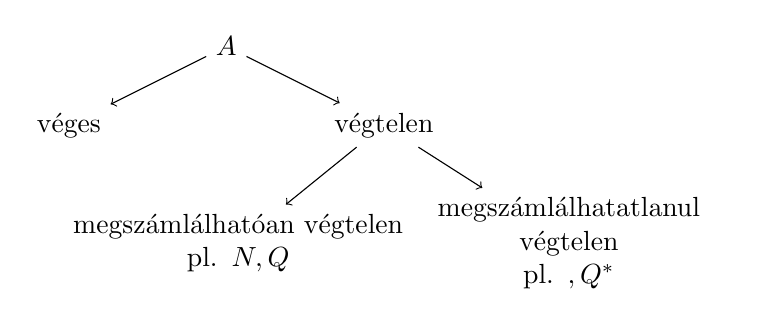
\begin{tikzpicture}
      % FIRST ROW
      \node (1) at (0,0) {$\card A$};

      % SECOND ROW
      \node (21) at (-2,-1) {véges};
      \node (22) at (2,-1) {végtelen};

      % CONNECT 1 -> 2
      \draw[->] (1) -- (21);
      \draw[->] (1) -- (22);

      % THIRD ROW
      \node[text width=4.5cm, align=center] (31) at (0.15,-2.5)
      {megszámlálhatóan végtelen\\pl. $\mathbb N, \mathbb Q$};
      \node[text width=4.5cm, align=center] (32) at (4.35,-2.5)
      {megszámlálhatatlanul végtelen\\pl. $\Reals, \mathbb Q^*$};

      % CONNECT 2 -> 3
      \draw[->] (22) -- (31);
      \draw[->] (22) -- (32);
    \end{tikzpicture}
  \end{center}
\end{note}

\begin{theorem}[Racionális számok halmazának számossága]
  A racionális számok halmaza megszámlálhatóan végtelen.

  \begin{proof}[Cantor átlós módszere]
    \begin{minipage}{.5\textwidth}
      Minden pozitív racionális szám felírható tört alakban, ahol a nevező és a
      számláló is egész szám, ráadásul ezek relatív prímek.
      \\[.33em]
      Ezeket a törteket rendezzük egy olyan táblázatba, ahol az $n$ sorban az
      $m$ oszlopban az $\sfrac{m}{n}$ tört áll. Ezeket a törteket az ábrán
      jelöl módszerrel sorba állítjuk, sorrendjük szerint pedig egyértelműen
      megfeleltethetők a természetes számoknak.
      \\[.33em]
      Könnyen belátható, hogy ez a módszer az összes racionális számra
      is kiterjeszthető, tehát a racionális számok halmaza valóban
      megszámlálhatóan végtelen.
      %\begin{noindent}
    \end{minipage}\hfill%
    \begin{minipage}{.425\textwidth}
      % \end{noindent}
      \begin{tikzpicture}[
          decoration={
              markings,
              mark=at position 0.5 with {\arrow{>}
                }
            }
        ]
        \draw[ultra thick, secondaryColor] (.5,-.5) rectangle (6.5,-7.5);

        \foreach \y in {1,...,6}{
            \foreach \x in {1,...,5}{
                \node (\x\y) at (\x,-\y) {$\sfrac{\x}{\y}$};
              }
          }

        \foreach \y in {1,...,6} {
            \node (6\y) at (6,-\y) {$\hdots$};
          }
        \foreach \x in {1,...,5}{
            \node (\x7) at (\x,-7) {$\vdots$};
          }
        \node(67) at (6,-7) {$\ddots$};

        \coordinate (P) at (11);
        \foreach \c in {12, 21, 31, 22, 13, 14, 23, 32, 41, 51, 42, 33, 24, 15, 16, 25, 34, 43, 52, 61}{
            \draw[postaction={decorate}, primaryColor, thick, opacity=0.5] (P) -- (\c.center);
            \coordinate (P) at (\c);
          }
      \end{tikzpicture}
    \end{minipage}
  \end{proof}
\end{theorem}

% \begin{theorem}[Valós számok halmazának számossága]
%   A valós számok halmaza nem megszámlálhatóan végtelen.
% \end{theorem}

% Ponthalmazok
\begin{blueBox}
  \sftitle{Fontosabb jelölések:}
  \begin{itemize}
    \item Nyílt halmaz jelölése: $(x; y) = ]x; y[$.
    \item Zárt halmaz jelölése: $[x; y]$.
    \item Az $a$ pont $\varepsilon$ sugarú környezete: $K(a; \varepsilon) := (a
          - \varepsilon; a + \varepsilon)$ \\ (ezzel ekvivalens: $|x-a| <
          \varepsilon$).
  \end{itemize}

  \begin{center}
    \begin{tikzpicture}
      % ARROW
      \draw[-to, ultra thick, secondaryColor] (-2,0) -- (2,0);

      % a point
      \draw[draw=primaryColor, ultra thick] (0,-1mm) -- ++(0,2mm)
      node[above] {$a$};

      % OPEN INTERVAL
      \draw[draw=primaryColor, ultra thick] (+10:1.25) arc (+10:-10:1.25)
      node[below] {$a + \varepsilon$};
      \draw[draw=primaryColor, ultra thick] (170:1.25) arc (170:190:1.25)
      node[below] {$a - \varepsilon$};
    \end{tikzpicture}
  \end{center}
\end{blueBox}

\begin{definition}[Alsó és felső korlát]
  A felülről korlátos $H$ halmaz legkisebb felső korlátja: supremum, jele: $\sup
    H$.
  \\
  Az alulról korlátos $H$ halmaz legnagyobb alsó korlátja: infimum, jele: $\inf
    H$.
\end{definition}

\begin{theorem}[Korlátos halmaz szuprémuma]
  Felülről korlátos nemüres halmaznak mindig van szuprémuma.
\end{theorem}

\begin{theorem}[Korlátos halmaz infimuma]
  Alulról korlátos nemüres halmaznak mindig van infimuma.
\end{theorem}
\vfill
\begin{questions}[section.1.5]
  \begin{enumerate}
    \item Mikor mondjuk, hogy egy halmaz jól definiált?

    \item Válassza ki az alábbi halmazok közül azokat, amelyek jól definiáltak!
          \begin{enumerate}
            \item A magas férfihallgatók,
            \item azon valós számok, amelyek négyzete nem kisebb háromnál,
            \item a viharos erejű szelek,
            \item a poliéderek.
          \end{enumerate}

    \item Definiálja a következő fogalmakat: üreshalmaz, halmaz komplementere,
          részhalmaz, halmazok metszete, uniója

    \item Definiálja két halmaz Descartes-szorzatát!

    \item Hány részhalmaza van egy $n$ elemű halmaznak?

    \item Zárt-e az irracionális számok halmaza az összeadásra nézve?

    \item Alulról korlátos-e a természetes számok halmaza? És felülről?

    \item Adjon példát véges halmazokra!

    \item Adjon példát megszámlálhatóan végtelen számosságú halmazokra!
  \end{enumerate}
\end{questions}


\mainChapter{Vektoranalízis}\label{chap-01}

\bgroup
\color{gray!50!black}
\sffamily

% Lorem ipsum

\chaptertoc
\egroup

\clearpage
\section{Fogalmak, definíciók}

\begin{blueBox}
  Tekintsük a következő egyenletrendszert:
  \[
    \begin{cases}
      x + y = -10 \\
      x \cdot y = 40
    \end{cases}
  \]

  Az egyenletrendszert megoldva az alábbi megoldásokat kapjuk:
  \[
    \begin{cases}
      x = -5 + \sqrt{-15} \\
      y = -5 - \sqrt{-15}
    \end{cases}
    \quad
    \begin{cases}
      x = -5 - \sqrt{-15} \\
      y = -5 + \sqrt{-15}
    \end{cases}
  \]

  Mit jelent, ha a négyzetgyökjel alatt negatív számot kapunk?

  Bővítsük a valós számok halmazát! Legyen $\iu^2 = -1$.

  A komplex számokat az úgynevezett Gauss-számsíkon ábrázoljuk.

  \begin{center}
    \begin{tikzpicture}[thick, scale=0.75]
      \draw[->] (-.5, 0) -- (3, 0) node[right] {$\Re$};
      \draw[->] (0, -.5) -- (0, 3) node[above] {$\Im$};

      \draw[draw=gray, dashed]
      (1.5,0) node[below] {$a$}
      -- (1.5, 2.5)
      -- (0, 2.5) node[left] {$b$};

      \draw[fill=primaryColor] (1.5, 2.5) circle (0.1)
      node[above right] {$z = a + b\iu$};
    \end{tikzpicture}
  \end{center}

  A komplex számok halmazának jele: $\mathbb C$.

  \textbf{Algebrai alak}: $z = a + b\iu$, ahol $a, b \in \Reals$.

  A komplex szám \textbf{valós része}: $\iRe z = \{a\}$.

  A komplex szám \textbf{képzetes része} pedig $\iIm \{z\} = b$.
\end{blueBox}

\begin{note}
  A komplex számok halmaza és a valós számok halmazának önmagával vett
  Descartes-szorzata között kölcsönösen egyértelmű megfeleltetés van, vagyis:
  $\mathbb C \cong \Reals \times \Reals$.
\end{note}

\begin{definition}[Két komplex szám egyenlősége]
  Legyenek $z_1 = a_1 + b_1\iu$ és $z_2 = a_2 + b_2\iu$ komplex számok. Ekkor:
  \[
    z_1 = z_2
    \quad \Leftrightarrow \quad
    a_1 = a_2 \quad \text{és} \quad b_1 = b_2
    \text.
  \]
\end{definition}

\begin{definition}[Komplex számok összege]
  Legyenek $z_1 = a_1 + b_1\iu$ és $z_2 = a_2 + b_2\iu$ komplex számok. Ekkor:
  \[
    z_1 + z_2 = (a_1 + a_2) + (b_1 + b_2)\iu
    \text.
  \]
\end{definition}

\begin{definition}[Konjugált]
  Legyen $z = a + b\iu$ egy komplex szám. Ekkor $z$ konjugáltja:
  \[
    \overline{z} = a - b\iu
    \text.
  \]
\end{definition}

\begin{note}
  Komplex szám és konjugáltjának összege valós szám:
  $z + \overline{z} = 2 a \in \Reals$.
  % \end{note}

  % \begin{note}
  Komplex szám és konjugáltjának szorzata valós szám:
  $z \cdot \overline{z} = a^2 + b^2 \in \Reals$.
\end{note}

\begin{definition}[Két komplex szám szorzata]
  \vspace{-1.5em}
  \begin{align*}
    z_1 \cdot z_2
     & = (a_1 + b_1\iu) \cdot (a_2 + b_2\iu)              \\
     & = a_1 a_2 + a_1 b_2\iu + a_2 b_1\iu + b_1 b_2\iu^2 \\
     & = (a_1 a_2 - b_1 b_2) + (a_1 b_2 + a_2 b_1)\iu
  \end{align*}
\end{definition}

\begin{blueBox}
  \sftitle{Áttérés a polárkoordináta-rendszerre:}

  Általában a Descartes-féle koordinátarendszerben dolgozunk, ahol a sík pontjai
  és a számpárok között kölcsönösen egyértelmű megfeleltetés van. Időnként
  azonban célravezető más koordinátarendszerek alkalmazása is.

  \begin{center}
    \begin{tikzpicture}[scale=3/4]
      % Draw the lines at multiples of pi/12
      \foreach \ang in {0,...,31} {
          \draw [lightgray] (0,0) -- (\ang * 180 / 16:4.1);
        }

      % Concentric circles
      \foreach \s in {0, 1, 2, 3} {
          \draw [lightgray] (0,0) circle (\s + 0.5);
          \draw [primaryColor] (0,0) circle (\s);
        }

      % Add the labels at multiples of pi/4
      \foreach \ang/\lab/\dir in {
      % 0/0/right,
      1/{\pi/4}/{above right},
      2/{\pi/2}/above,
      3/{3\pi/4}/{above left},
      4/{\pi}/left,
      5/{5\pi/4}/{below left},
      7/{7\pi/4}/{below right},
      6/{3\pi/2}/below} {
      \draw (0,0) -- (\ang * 180 / 4:4.5);
      \node [fill=cyan!10] at (\ang * 180 / 4:4.35) [\dir] {$\lab$};
      }

      % Outer circle
      \draw (0,0) circle (4);

      % 0 angle line
      \draw [-to, ultra thick] (0,0) -- (6,0) node [above left] {$r$};
      \node [above right] at (4,0) {$0$};

      % Radius labels
      \foreach \lab in {0, 1, 2, 3, 4} {
          \node [fill=cyan!10, inner sep=2pt, outer sep=2pt] at (\lab, 0)
          [below right] {\lab};
        }

      % Example
      \draw[secondaryColor, ultra thick] (0,0) -- (60:3);
      \draw[secondaryColor, thick] (0,0) -- ++(150:.5);
      \draw[secondaryColor, thick] (60:3) -- ++(150:.5);

      \draw[draw=primaryColor, ultra thick, to-to] (150:.35) -- ++(60:3)
      node[midway, above, fill=cyan!10, rotate=60, inner sep=2pt, outer sep=2pt]
      {$r$};

      \draw[ultra thick, primaryColor, -to] (1.4,0) arc
        [start angle=0, end angle=60, radius=1.4cm];

      \node[fill=cyan!10, inner sep=2pt, outer sep=2pt] at (30:.85) {$\varphi$};

      \draw[fill=primaryColor] (60:3) circle (0.1)
      node[below right, fill=cyan!10, inner sep=2pt, outer sep=5pt]
        {$z = r(\cos \varphi + \iu \sin \varphi)$};
    \end{tikzpicture}
  \end{center}

  Ebben az esetben a komplex szám szögfüggvények segítségével fejezhető ki:
  \[
    z = r (\cos \varphi + \iu \sin \varphi)
    \text.
  \]

  Az algebrai és trigonometrikus alak közötti kapcsolat:
  \[
    \begin{cases}
      a = r \cos \varphi \\
      b = r \sin \varphi
    \end{cases}
    \hspace{3cm}
    \begin{cases}
      r = \sqrt{a^2 + b^2} \\
      \varphi = \arctan(b / a)
    \end{cases}
  \]

  Ezek alapján $z_1 = r_1 (\cos \varphi_1 + \iu \sin \varphi_1)$ és $z_2 = r_2 (
    \cos \varphi_2 + \iu \sin \varphi_2)$ komplex számok szorzata trigonometrikus
  azonosságok segítségével:
  \begin{align*}
    z_1 \cdot z_2
     & = r_1 (\cos \varphi_1 + \iu \sin \varphi_1) \cdot
    r_2 (\cos \varphi_2 + \iu \sin \varphi_2)
    \\
     & = r_1 r_2 (\cos \varphi_1 \cos \varphi_2 - \sin \varphi_1 \sin \varphi_2) +
    r_1 r_2 (\cos \varphi_1 \sin \varphi_2 + \sin \varphi_1 \cos \varphi_2) \iu
    \\
     & = r_1 r_2 \left(
    \cos(\varphi_1 + \varphi_2) + \iu \sin(\varphi_1 + \varphi_2)
    \right)
    \text.
  \end{align*}

  A felhasznált azonosságok:
  \begin{align*}
    \sin(\alpha + \beta) & = \cos \alpha \sin \beta + \sin \alpha \cos \beta
    \text,                                                                   \\
    \cos(\alpha + \beta) & =\cos \alpha \cos \beta - \sin \alpha \sin \beta
    \text.
  \end{align*}
\end{blueBox}

\begin{blueBox}
  \sftitle{Komplex számok hatványozása:}
  \[
    z^n
    = (r(\cos \varphi + \iu \sin \varphi))^n
    = r^n (\cos (n \varphi) + \iu \sin (n \varphi))
  \]

  \begin{proof}[Teljes indukció módszerével]
    Vizsgáljuk meg az első pár esetet:
    \begin{align*}
      z^1 & = r^1 (\cos \varphi + \iu \sin \varphi) \text,                                                                                         \\
      z^2 & = r^2 (\cos \varphi + \iu \sin \varphi)^2                                                                                              \\
          & = r^2 (\cos^2 \varphi - \sin^2 \varphi + 2\iu \cos \varphi \sin \varphi)                                                               \\
          & = r^2 (\cos (2\varphi) + \iu \sin (2\varphi)) \text,                                                                                   \\
      z^3 & = z^2 \cdot z                                                                                                                          \\
          & = r^2 (\cos (2\varphi) + \iu \sin (2\varphi)) \cdot r(\cos \varphi + \iu \sin \varphi)                                                 \\
          & = r^3 (\cos (2\varphi) \cos \varphi - \sin (2\varphi) \sin \varphi + \iu (\cos (2\varphi) \sin \varphi + \sin (2\varphi) \cos \varphi) \\
          & = r^3 (\cos (3\varphi) + \iu \sin (3\varphi)) \text.
    \end{align*}

    Tegyük fel, hogy $z^k = r^k (\cos k\varphi + \iu \sin k\varphi)$, majd
    vizsgáljuk meg az $(n + 1)$-edik esetet:
    \begin{align*}
      z^{k + 1}
       & = z^k \cdot z
      = r^k (\cos (k\varphi) + \iu \sin (k\varphi)) \cdot r(\cos \varphi + \iu \sin \varphi)
      \\
       & = r^{k + 1} (\cos (k\varphi) \cos \varphi - \sin (k\varphi) \sin \varphi + \iu \cos (k\varphi) \sin \varphi + \sin (k\varphi) \cos \varphi)
      \\
       & = r^{k + 1} (\cos ((k + 1)\varphi) + \iu \sin ((k + 1)\varphi))
      \text.
    \end{align*}

    Ezzel bebizonyítottuk, hogy $z^n = r^n (\cos n\varphi + \iu \sin n\varphi)$.
  \end{proof}
\end{blueBox}

\begin{blueBox}
  \sftitle{Komplex számok osztása:}
  \[
    \frac{z_1}{z_2}
    = \frac{
      r_1 (\cos \varphi_1 + \iu \sin \varphi_1)
    }{
      r_2 (\cos \varphi_2 + \iu \sin \varphi_2)
    }
    = \frac{r_1}{r_2} (\cos (\varphi_1 - \varphi_2) + \iu \sin (\varphi_1 - \varphi_2))
  \]
\end{blueBox}

\begin{blueBox}
  \sftitle{Komplex számok gyökvonása:}
  \[
    \sqrt[n]{z}
    % = \sqrt[n]{r(\cos \varphi + \iu \sin \varphi)}
    = \sqrt[n]{r} \left(
    \cos \left( \frac{\varphi + 2k\pi}{n} \right) + \iu \sin \left( \frac{\varphi + 2k\pi}{n} \right)
    \right)
    \;
    k \in \{0; 1; \ldots; n-1\}
  \]
\end{blueBox}

\begin{note}
  Tetszőleges komplex szám $n$-edik gyökei egy olyan szabályos $n$-szög csúcsai,
  amelynek középpontja az origó.
  \begin{center}
    \begin{tikzpicture}[ultra thick]
      % COORDINATE SYSTEM
      \draw[-to, draw=primaryColor] (-2, 0) -- (2, 0) node [right] {$\Re$};
      \draw[-to, draw=primaryColor] (0, -2) -- (0, 2) node [above] {$\Im$};

      \coordinate (P) at (318:1.5);
      \foreach \deg in {30,102,174,246,318} {
          \draw[draw=primaryColor] (\deg:1.5) coordinate(C) circle (0.1);
          \draw[dashed, gray] (P) -- (C);
          \coordinate (P) at (C);
        }
    \end{tikzpicture}
  \end{center}
\end{note}

\begin{note}
  A komplex számokat nem tudjuk rendezni, azonban $(\mathbb C, +, \cdot)$
  test.
\end{note}

\begin{theorem}[Az algebra alaptétele]
  Egy $n$-ed fokú komplex együtthatós polinomnak multiplicitással számolva
  pontosan $n$ darab gyöke van.
\end{theorem}

\begin{note}
  Minden valós együtthatós polinom felírható első és másodfokú tényezők
  szorzataként.
\end{note}
\vfill
\begin{questions}[section.2.2]
  \begin{enumerate}
    \item Mit értünk egy komplex szám algebrai, trigonometrikus és exponenciális
          alakján?
          %     \item Mit értünk egy komplex szám trigonometrikus alakján?
          %     \item Mit értünk egy komplex szám exponenciális alakján?
    \item Adja meg a komplex számok különböző alakjai közötti áttéréseket!
    \item Definiálja a komplex számok halmazán az összeadás és a szorzás
          műveletét! Milyen struktúrát alkotnak a komplex számok az összeadásra
          és a szorzásra nézve?
    \item Adja meg a test definícióját, említsen példákat!
    \item Ismertesse a komplex számok hatványozására vonatkozó képletet!
    \item Ismertesse a komplex számok gyökvonására vonatkozó formulát!
    \item Hogyan helyezkednek egy komplex szám n. Gyökei a komplex számsíkon?
    \item Mit jelent az $n$-edik egységgyök?
  \end{enumerate}
\end{questions}


\mainChapter{Vektoranalízis}\label{chap-01}

\bgroup
\color{gray!50!black}
\sffamily

% Lorem ipsum

\chaptertoc
\egroup

\clearpage
\section{Fogalmak, definíciók}

\begin{blueBox}
  Tekintsük a következő egyenletrendszert:
  \[
    \begin{cases}
      x + y = -10 \\
      x \cdot y = 40
    \end{cases}
  \]

  Az egyenletrendszert megoldva az alábbi megoldásokat kapjuk:
  \[
    \begin{cases}
      x = -5 + \sqrt{-15} \\
      y = -5 - \sqrt{-15}
    \end{cases}
    \quad
    \begin{cases}
      x = -5 - \sqrt{-15} \\
      y = -5 + \sqrt{-15}
    \end{cases}
  \]

  Mit jelent, ha a négyzetgyökjel alatt negatív számot kapunk?

  Bővítsük a valós számok halmazát! Legyen $\iu^2 = -1$.

  A komplex számokat az úgynevezett Gauss-számsíkon ábrázoljuk.

  \begin{center}
    \begin{tikzpicture}[thick, scale=0.75]
      \draw[->] (-.5, 0) -- (3, 0) node[right] {$\Re$};
      \draw[->] (0, -.5) -- (0, 3) node[above] {$\Im$};

      \draw[draw=gray, dashed]
      (1.5,0) node[below] {$a$}
      -- (1.5, 2.5)
      -- (0, 2.5) node[left] {$b$};

      \draw[fill=primaryColor] (1.5, 2.5) circle (0.1)
      node[above right] {$z = a + b\iu$};
    \end{tikzpicture}
  \end{center}

  A komplex számok halmazának jele: $\mathbb C$.

  \textbf{Algebrai alak}: $z = a + b\iu$, ahol $a, b \in \Reals$.

  A komplex szám \textbf{valós része}: $\iRe z = \{a\}$.

  A komplex szám \textbf{képzetes része} pedig $\iIm \{z\} = b$.
\end{blueBox}

\begin{note}
  A komplex számok halmaza és a valós számok halmazának önmagával vett
  Descartes-szorzata között kölcsönösen egyértelmű megfeleltetés van, vagyis:
  $\mathbb C \cong \Reals \times \Reals$.
\end{note}

\begin{definition}[Két komplex szám egyenlősége]
  Legyenek $z_1 = a_1 + b_1\iu$ és $z_2 = a_2 + b_2\iu$ komplex számok. Ekkor:
  \[
    z_1 = z_2
    \quad \Leftrightarrow \quad
    a_1 = a_2 \quad \text{és} \quad b_1 = b_2
    \text.
  \]
\end{definition}

\begin{definition}[Komplex számok összege]
  Legyenek $z_1 = a_1 + b_1\iu$ és $z_2 = a_2 + b_2\iu$ komplex számok. Ekkor:
  \[
    z_1 + z_2 = (a_1 + a_2) + (b_1 + b_2)\iu
    \text.
  \]
\end{definition}

\begin{definition}[Konjugált]
  Legyen $z = a + b\iu$ egy komplex szám. Ekkor $z$ konjugáltja:
  \[
    \overline{z} = a - b\iu
    \text.
  \]
\end{definition}

\begin{note}
  Komplex szám és konjugáltjának összege valós szám:
  $z + \overline{z} = 2 a \in \Reals$.
  % \end{note}

  % \begin{note}
  Komplex szám és konjugáltjának szorzata valós szám:
  $z \cdot \overline{z} = a^2 + b^2 \in \Reals$.
\end{note}

\begin{definition}[Két komplex szám szorzata]
  \vspace{-1.5em}
  \begin{align*}
    z_1 \cdot z_2
     & = (a_1 + b_1\iu) \cdot (a_2 + b_2\iu)              \\
     & = a_1 a_2 + a_1 b_2\iu + a_2 b_1\iu + b_1 b_2\iu^2 \\
     & = (a_1 a_2 - b_1 b_2) + (a_1 b_2 + a_2 b_1)\iu
  \end{align*}
\end{definition}

\begin{blueBox}
  \sftitle{Áttérés a polárkoordináta-rendszerre:}

  Általában a Descartes-féle koordinátarendszerben dolgozunk, ahol a sík pontjai
  és a számpárok között kölcsönösen egyértelmű megfeleltetés van. Időnként
  azonban célravezető más koordinátarendszerek alkalmazása is.

  \begin{center}
    \begin{tikzpicture}[scale=3/4]
      % Draw the lines at multiples of pi/12
      \foreach \ang in {0,...,31} {
          \draw [lightgray] (0,0) -- (\ang * 180 / 16:4.1);
        }

      % Concentric circles
      \foreach \s in {0, 1, 2, 3} {
          \draw [lightgray] (0,0) circle (\s + 0.5);
          \draw [primaryColor] (0,0) circle (\s);
        }

      % Add the labels at multiples of pi/4
      \foreach \ang/\lab/\dir in {
      % 0/0/right,
      1/{\pi/4}/{above right},
      2/{\pi/2}/above,
      3/{3\pi/4}/{above left},
      4/{\pi}/left,
      5/{5\pi/4}/{below left},
      7/{7\pi/4}/{below right},
      6/{3\pi/2}/below} {
      \draw (0,0) -- (\ang * 180 / 4:4.5);
      \node [fill=cyan!10] at (\ang * 180 / 4:4.35) [\dir] {$\lab$};
      }

      % Outer circle
      \draw (0,0) circle (4);

      % 0 angle line
      \draw [-to, ultra thick] (0,0) -- (6,0) node [above left] {$r$};
      \node [above right] at (4,0) {$0$};

      % Radius labels
      \foreach \lab in {0, 1, 2, 3, 4} {
          \node [fill=cyan!10, inner sep=2pt, outer sep=2pt] at (\lab, 0)
          [below right] {\lab};
        }

      % Example
      \draw[secondaryColor, ultra thick] (0,0) -- (60:3);
      \draw[secondaryColor, thick] (0,0) -- ++(150:.5);
      \draw[secondaryColor, thick] (60:3) -- ++(150:.5);

      \draw[draw=primaryColor, ultra thick, to-to] (150:.35) -- ++(60:3)
      node[midway, above, fill=cyan!10, rotate=60, inner sep=2pt, outer sep=2pt]
      {$r$};

      \draw[ultra thick, primaryColor, -to] (1.4,0) arc
        [start angle=0, end angle=60, radius=1.4cm];

      \node[fill=cyan!10, inner sep=2pt, outer sep=2pt] at (30:.85) {$\varphi$};

      \draw[fill=primaryColor] (60:3) circle (0.1)
      node[below right, fill=cyan!10, inner sep=2pt, outer sep=5pt]
        {$z = r(\cos \varphi + \iu \sin \varphi)$};
    \end{tikzpicture}
  \end{center}

  Ebben az esetben a komplex szám szögfüggvények segítségével fejezhető ki:
  \[
    z = r (\cos \varphi + \iu \sin \varphi)
    \text.
  \]

  Az algebrai és trigonometrikus alak közötti kapcsolat:
  \[
    \begin{cases}
      a = r \cos \varphi \\
      b = r \sin \varphi
    \end{cases}
    \hspace{3cm}
    \begin{cases}
      r = \sqrt{a^2 + b^2} \\
      \varphi = \arctan(b / a)
    \end{cases}
  \]

  Ezek alapján $z_1 = r_1 (\cos \varphi_1 + \iu \sin \varphi_1)$ és $z_2 = r_2 (
    \cos \varphi_2 + \iu \sin \varphi_2)$ komplex számok szorzata trigonometrikus
  azonosságok segítségével:
  \begin{align*}
    z_1 \cdot z_2
     & = r_1 (\cos \varphi_1 + \iu \sin \varphi_1) \cdot
    r_2 (\cos \varphi_2 + \iu \sin \varphi_2)
    \\
     & = r_1 r_2 (\cos \varphi_1 \cos \varphi_2 - \sin \varphi_1 \sin \varphi_2) +
    r_1 r_2 (\cos \varphi_1 \sin \varphi_2 + \sin \varphi_1 \cos \varphi_2) \iu
    \\
     & = r_1 r_2 \left(
    \cos(\varphi_1 + \varphi_2) + \iu \sin(\varphi_1 + \varphi_2)
    \right)
    \text.
  \end{align*}

  A felhasznált azonosságok:
  \begin{align*}
    \sin(\alpha + \beta) & = \cos \alpha \sin \beta + \sin \alpha \cos \beta
    \text,                                                                   \\
    \cos(\alpha + \beta) & =\cos \alpha \cos \beta - \sin \alpha \sin \beta
    \text.
  \end{align*}
\end{blueBox}

\begin{blueBox}
  \sftitle{Komplex számok hatványozása:}
  \[
    z^n
    = (r(\cos \varphi + \iu \sin \varphi))^n
    = r^n (\cos (n \varphi) + \iu \sin (n \varphi))
  \]

  \begin{proof}[Teljes indukció módszerével]
    Vizsgáljuk meg az első pár esetet:
    \begin{align*}
      z^1 & = r^1 (\cos \varphi + \iu \sin \varphi) \text,                                                                                         \\
      z^2 & = r^2 (\cos \varphi + \iu \sin \varphi)^2                                                                                              \\
          & = r^2 (\cos^2 \varphi - \sin^2 \varphi + 2\iu \cos \varphi \sin \varphi)                                                               \\
          & = r^2 (\cos (2\varphi) + \iu \sin (2\varphi)) \text,                                                                                   \\
      z^3 & = z^2 \cdot z                                                                                                                          \\
          & = r^2 (\cos (2\varphi) + \iu \sin (2\varphi)) \cdot r(\cos \varphi + \iu \sin \varphi)                                                 \\
          & = r^3 (\cos (2\varphi) \cos \varphi - \sin (2\varphi) \sin \varphi + \iu (\cos (2\varphi) \sin \varphi + \sin (2\varphi) \cos \varphi) \\
          & = r^3 (\cos (3\varphi) + \iu \sin (3\varphi)) \text.
    \end{align*}

    Tegyük fel, hogy $z^k = r^k (\cos k\varphi + \iu \sin k\varphi)$, majd
    vizsgáljuk meg az $(n + 1)$-edik esetet:
    \begin{align*}
      z^{k + 1}
       & = z^k \cdot z
      = r^k (\cos (k\varphi) + \iu \sin (k\varphi)) \cdot r(\cos \varphi + \iu \sin \varphi)
      \\
       & = r^{k + 1} (\cos (k\varphi) \cos \varphi - \sin (k\varphi) \sin \varphi + \iu \cos (k\varphi) \sin \varphi + \sin (k\varphi) \cos \varphi)
      \\
       & = r^{k + 1} (\cos ((k + 1)\varphi) + \iu \sin ((k + 1)\varphi))
      \text.
    \end{align*}

    Ezzel bebizonyítottuk, hogy $z^n = r^n (\cos n\varphi + \iu \sin n\varphi)$.
  \end{proof}
\end{blueBox}

\begin{blueBox}
  \sftitle{Komplex számok osztása:}
  \[
    \frac{z_1}{z_2}
    = \frac{
      r_1 (\cos \varphi_1 + \iu \sin \varphi_1)
    }{
      r_2 (\cos \varphi_2 + \iu \sin \varphi_2)
    }
    = \frac{r_1}{r_2} (\cos (\varphi_1 - \varphi_2) + \iu \sin (\varphi_1 - \varphi_2))
  \]
\end{blueBox}

\begin{blueBox}
  \sftitle{Komplex számok gyökvonása:}
  \[
    \sqrt[n]{z}
    % = \sqrt[n]{r(\cos \varphi + \iu \sin \varphi)}
    = \sqrt[n]{r} \left(
    \cos \left( \frac{\varphi + 2k\pi}{n} \right) + \iu \sin \left( \frac{\varphi + 2k\pi}{n} \right)
    \right)
    \;
    k \in \{0; 1; \ldots; n-1\}
  \]
\end{blueBox}

\begin{note}
  Tetszőleges komplex szám $n$-edik gyökei egy olyan szabályos $n$-szög csúcsai,
  amelynek középpontja az origó.
  \begin{center}
    \begin{tikzpicture}[ultra thick]
      % COORDINATE SYSTEM
      \draw[-to, draw=primaryColor] (-2, 0) -- (2, 0) node [right] {$\Re$};
      \draw[-to, draw=primaryColor] (0, -2) -- (0, 2) node [above] {$\Im$};

      \coordinate (P) at (318:1.5);
      \foreach \deg in {30,102,174,246,318} {
          \draw[draw=primaryColor] (\deg:1.5) coordinate(C) circle (0.1);
          \draw[dashed, gray] (P) -- (C);
          \coordinate (P) at (C);
        }
    \end{tikzpicture}
  \end{center}
\end{note}

\begin{note}
  A komplex számokat nem tudjuk rendezni, azonban $(\mathbb C, +, \cdot)$
  test.
\end{note}

\begin{theorem}[Az algebra alaptétele]
  Egy $n$-ed fokú komplex együtthatós polinomnak multiplicitással számolva
  pontosan $n$ darab gyöke van.
\end{theorem}

\begin{note}
  Minden valós együtthatós polinom felírható első és másodfokú tényezők
  szorzataként.
\end{note}
\section{Nevezetes sorozatok}

\begin{theorem}[Bernoulli-egyenlőtlenség]
  Ha $x \geq -1$, akkor: $(1 + x)^n \geq 1 + n \cdot x$, $\forall n \in
    \mathbb N$, az egyenlőség akkor és csakis akkor teljesül, ha $n = 0$,
  $n = 1$, vagy $x = 0$.
\end{theorem}

\begin{blueBox}
  $
    a^n \rightarrow \begin{cases}
      \;0,                & \text{ha } |a| < 1,   \\
      \;1,                & \text{ha } a = 1,     \\
      \;\infty,           & \text{ha } a > 1,     \\
      \;\text{divergens}, & \text{ha } a \leq -1.
    \end{cases}
  $

  \hdashrule[.8ex][x]{\dimexpr\textwidth}{1pt}{2mm 3pt}
  \phantom{alma}\vspace{10cm}\phantom{alma}


  % Ha $a > 1$, akkor $a = 1 + h$ alakban, ahol $h > 0$, és $a^n = (1 + h)^n
  %   \geq 1 + n \cdot h \rightarrow \infty$.

  % Ha $a = 1$, akkor $a^n = 1^n = 1$.

  % Ha $|a| < 1$, akkor $|a^n| = |a|^n = \dfrac{1}{\sfrac{1}{|a|^n}} \rightarrow 0$
\end{blueBox}

\begin{blueBox}
  $
    \sqrt[n]{a} \rightarrow 1
  $

  \hdashrule[.8ex][x]{\dimexpr\textwidth}{1pt}{2mm 3pt}
  \phantom{alma}\vspace{9.5cm}\phantom{alma}
\end{blueBox}

\begin{blueBox}
  $
    a^n \cdot n^k \rightarrow 0$
  \text{, ha }
  $|a|<1$
  \text{ és }
  $k \in \mathbb N
  $

  \hdashrule[.8ex][x]{\dimexpr\textwidth}{1pt}{2mm 3pt}
  \phantom{alma}\vspace{9.5cm}\phantom{alma}
\end{blueBox}

\begin{blueBox}
  $
    \sqrt[n]{n} \rightarrow 1
  $

  \hdashrule[.8ex][x]{\dimexpr\textwidth}{1pt}{2mm 3pt}
  \phantom{alma}\vspace{9.5cm}\phantom{alma}
\end{blueBox}

\begin{blueBox}
  $
    \dfrac{a^n}{n!} \rightarrow 0
  $

  \hdashrule[.8ex][x]{\dimexpr\textwidth}{1pt}{2mm 3pt}
  \phantom{alma}\vspace{9.5cm}\phantom{alma}
\end{blueBox}

\begin{blueBox}
  $
    \left(1 + \dfrac{1}{n}\right)^n \rightarrow e
  $

  \hdashrule[.8ex][x]{\dimexpr\textwidth}{1pt}{2mm 3pt}
  \phantom{alma}\vspace{12.5cm}\phantom{alma}
\end{blueBox}
\vfill
\begin{questions}[section.03.03]
  \begin{enumerate}
    \item Definiálja a torlódási pont fogalmát!
    \item Definiálja a konvergens sorozat fogalmát! Mikor mondunk egy sorozatot
          divergensnek?
    \item Ismertesse a nevezetes sorozatok határértékeit!
    \item Mikor mondunk egy sorozatot monoton növekvőnek, - csökkenőnek?
    \item Mikor nevezünk egy sorozatot korlátosnak?
    \item Mit mondhatunk a konvergens sorozatok és a műveletek kapcsolatáról?
    \item Adja meg a részsorozat fogalmát!
    \item Ismertesse a monoton korlátos sorozatok konvergenciájára vonatkozó
          tételt!
    \item Igaz-e, hogy bármely konvergens sorozat korlátos? Ha igen, miért? Mit
          mondhatunk a megfordításról?
    \item Ismertesse a rendőrtételt!
  \end{enumerate}
\end{questions}


\mainChapter{Vektoranalízis}\label{chap-01}

\bgroup
\color{gray!50!black}
\sffamily

% Lorem ipsum

\chaptertoc
\egroup

\clearpage
\section{Fogalmak, definíciók}

\begin{blueBox}
  Tekintsük a következő egyenletrendszert:
  \[
    \begin{cases}
      x + y = -10 \\
      x \cdot y = 40
    \end{cases}
  \]

  Az egyenletrendszert megoldva az alábbi megoldásokat kapjuk:
  \[
    \begin{cases}
      x = -5 + \sqrt{-15} \\
      y = -5 - \sqrt{-15}
    \end{cases}
    \quad
    \begin{cases}
      x = -5 - \sqrt{-15} \\
      y = -5 + \sqrt{-15}
    \end{cases}
  \]

  Mit jelent, ha a négyzetgyökjel alatt negatív számot kapunk?

  Bővítsük a valós számok halmazát! Legyen $\iu^2 = -1$.

  A komplex számokat az úgynevezett Gauss-számsíkon ábrázoljuk.

  \begin{center}
    \begin{tikzpicture}[thick, scale=0.75]
      \draw[->] (-.5, 0) -- (3, 0) node[right] {$\Re$};
      \draw[->] (0, -.5) -- (0, 3) node[above] {$\Im$};

      \draw[draw=gray, dashed]
      (1.5,0) node[below] {$a$}
      -- (1.5, 2.5)
      -- (0, 2.5) node[left] {$b$};

      \draw[fill=primaryColor] (1.5, 2.5) circle (0.1)
      node[above right] {$z = a + b\iu$};
    \end{tikzpicture}
  \end{center}

  A komplex számok halmazának jele: $\mathbb C$.

  \textbf{Algebrai alak}: $z = a + b\iu$, ahol $a, b \in \Reals$.

  A komplex szám \textbf{valós része}: $\iRe z = \{a\}$.

  A komplex szám \textbf{képzetes része} pedig $\iIm \{z\} = b$.
\end{blueBox}

\begin{note}
  A komplex számok halmaza és a valós számok halmazának önmagával vett
  Descartes-szorzata között kölcsönösen egyértelmű megfeleltetés van, vagyis:
  $\mathbb C \cong \Reals \times \Reals$.
\end{note}

\begin{definition}[Két komplex szám egyenlősége]
  Legyenek $z_1 = a_1 + b_1\iu$ és $z_2 = a_2 + b_2\iu$ komplex számok. Ekkor:
  \[
    z_1 = z_2
    \quad \Leftrightarrow \quad
    a_1 = a_2 \quad \text{és} \quad b_1 = b_2
    \text.
  \]
\end{definition}

\begin{definition}[Komplex számok összege]
  Legyenek $z_1 = a_1 + b_1\iu$ és $z_2 = a_2 + b_2\iu$ komplex számok. Ekkor:
  \[
    z_1 + z_2 = (a_1 + a_2) + (b_1 + b_2)\iu
    \text.
  \]
\end{definition}

\begin{definition}[Konjugált]
  Legyen $z = a + b\iu$ egy komplex szám. Ekkor $z$ konjugáltja:
  \[
    \overline{z} = a - b\iu
    \text.
  \]
\end{definition}

\begin{note}
  Komplex szám és konjugáltjának összege valós szám:
  $z + \overline{z} = 2 a \in \Reals$.
  % \end{note}

  % \begin{note}
  Komplex szám és konjugáltjának szorzata valós szám:
  $z \cdot \overline{z} = a^2 + b^2 \in \Reals$.
\end{note}

\begin{definition}[Két komplex szám szorzata]
  \vspace{-1.5em}
  \begin{align*}
    z_1 \cdot z_2
     & = (a_1 + b_1\iu) \cdot (a_2 + b_2\iu)              \\
     & = a_1 a_2 + a_1 b_2\iu + a_2 b_1\iu + b_1 b_2\iu^2 \\
     & = (a_1 a_2 - b_1 b_2) + (a_1 b_2 + a_2 b_1)\iu
  \end{align*}
\end{definition}

\begin{blueBox}
  \sftitle{Áttérés a polárkoordináta-rendszerre:}

  Általában a Descartes-féle koordinátarendszerben dolgozunk, ahol a sík pontjai
  és a számpárok között kölcsönösen egyértelmű megfeleltetés van. Időnként
  azonban célravezető más koordinátarendszerek alkalmazása is.

  \begin{center}
    \begin{tikzpicture}[scale=3/4]
      % Draw the lines at multiples of pi/12
      \foreach \ang in {0,...,31} {
          \draw [lightgray] (0,0) -- (\ang * 180 / 16:4.1);
        }

      % Concentric circles
      \foreach \s in {0, 1, 2, 3} {
          \draw [lightgray] (0,0) circle (\s + 0.5);
          \draw [primaryColor] (0,0) circle (\s);
        }

      % Add the labels at multiples of pi/4
      \foreach \ang/\lab/\dir in {
      % 0/0/right,
      1/{\pi/4}/{above right},
      2/{\pi/2}/above,
      3/{3\pi/4}/{above left},
      4/{\pi}/left,
      5/{5\pi/4}/{below left},
      7/{7\pi/4}/{below right},
      6/{3\pi/2}/below} {
      \draw (0,0) -- (\ang * 180 / 4:4.5);
      \node [fill=cyan!10] at (\ang * 180 / 4:4.35) [\dir] {$\lab$};
      }

      % Outer circle
      \draw (0,0) circle (4);

      % 0 angle line
      \draw [-to, ultra thick] (0,0) -- (6,0) node [above left] {$r$};
      \node [above right] at (4,0) {$0$};

      % Radius labels
      \foreach \lab in {0, 1, 2, 3, 4} {
          \node [fill=cyan!10, inner sep=2pt, outer sep=2pt] at (\lab, 0)
          [below right] {\lab};
        }

      % Example
      \draw[secondaryColor, ultra thick] (0,0) -- (60:3);
      \draw[secondaryColor, thick] (0,0) -- ++(150:.5);
      \draw[secondaryColor, thick] (60:3) -- ++(150:.5);

      \draw[draw=primaryColor, ultra thick, to-to] (150:.35) -- ++(60:3)
      node[midway, above, fill=cyan!10, rotate=60, inner sep=2pt, outer sep=2pt]
      {$r$};

      \draw[ultra thick, primaryColor, -to] (1.4,0) arc
        [start angle=0, end angle=60, radius=1.4cm];

      \node[fill=cyan!10, inner sep=2pt, outer sep=2pt] at (30:.85) {$\varphi$};

      \draw[fill=primaryColor] (60:3) circle (0.1)
      node[below right, fill=cyan!10, inner sep=2pt, outer sep=5pt]
        {$z = r(\cos \varphi + \iu \sin \varphi)$};
    \end{tikzpicture}
  \end{center}

  Ebben az esetben a komplex szám szögfüggvények segítségével fejezhető ki:
  \[
    z = r (\cos \varphi + \iu \sin \varphi)
    \text.
  \]

  Az algebrai és trigonometrikus alak közötti kapcsolat:
  \[
    \begin{cases}
      a = r \cos \varphi \\
      b = r \sin \varphi
    \end{cases}
    \hspace{3cm}
    \begin{cases}
      r = \sqrt{a^2 + b^2} \\
      \varphi = \arctan(b / a)
    \end{cases}
  \]

  Ezek alapján $z_1 = r_1 (\cos \varphi_1 + \iu \sin \varphi_1)$ és $z_2 = r_2 (
    \cos \varphi_2 + \iu \sin \varphi_2)$ komplex számok szorzata trigonometrikus
  azonosságok segítségével:
  \begin{align*}
    z_1 \cdot z_2
     & = r_1 (\cos \varphi_1 + \iu \sin \varphi_1) \cdot
    r_2 (\cos \varphi_2 + \iu \sin \varphi_2)
    \\
     & = r_1 r_2 (\cos \varphi_1 \cos \varphi_2 - \sin \varphi_1 \sin \varphi_2) +
    r_1 r_2 (\cos \varphi_1 \sin \varphi_2 + \sin \varphi_1 \cos \varphi_2) \iu
    \\
     & = r_1 r_2 \left(
    \cos(\varphi_1 + \varphi_2) + \iu \sin(\varphi_1 + \varphi_2)
    \right)
    \text.
  \end{align*}

  A felhasznált azonosságok:
  \begin{align*}
    \sin(\alpha + \beta) & = \cos \alpha \sin \beta + \sin \alpha \cos \beta
    \text,                                                                   \\
    \cos(\alpha + \beta) & =\cos \alpha \cos \beta - \sin \alpha \sin \beta
    \text.
  \end{align*}
\end{blueBox}

\begin{blueBox}
  \sftitle{Komplex számok hatványozása:}
  \[
    z^n
    = (r(\cos \varphi + \iu \sin \varphi))^n
    = r^n (\cos (n \varphi) + \iu \sin (n \varphi))
  \]

  \begin{proof}[Teljes indukció módszerével]
    Vizsgáljuk meg az első pár esetet:
    \begin{align*}
      z^1 & = r^1 (\cos \varphi + \iu \sin \varphi) \text,                                                                                         \\
      z^2 & = r^2 (\cos \varphi + \iu \sin \varphi)^2                                                                                              \\
          & = r^2 (\cos^2 \varphi - \sin^2 \varphi + 2\iu \cos \varphi \sin \varphi)                                                               \\
          & = r^2 (\cos (2\varphi) + \iu \sin (2\varphi)) \text,                                                                                   \\
      z^3 & = z^2 \cdot z                                                                                                                          \\
          & = r^2 (\cos (2\varphi) + \iu \sin (2\varphi)) \cdot r(\cos \varphi + \iu \sin \varphi)                                                 \\
          & = r^3 (\cos (2\varphi) \cos \varphi - \sin (2\varphi) \sin \varphi + \iu (\cos (2\varphi) \sin \varphi + \sin (2\varphi) \cos \varphi) \\
          & = r^3 (\cos (3\varphi) + \iu \sin (3\varphi)) \text.
    \end{align*}

    Tegyük fel, hogy $z^k = r^k (\cos k\varphi + \iu \sin k\varphi)$, majd
    vizsgáljuk meg az $(n + 1)$-edik esetet:
    \begin{align*}
      z^{k + 1}
       & = z^k \cdot z
      = r^k (\cos (k\varphi) + \iu \sin (k\varphi)) \cdot r(\cos \varphi + \iu \sin \varphi)
      \\
       & = r^{k + 1} (\cos (k\varphi) \cos \varphi - \sin (k\varphi) \sin \varphi + \iu \cos (k\varphi) \sin \varphi + \sin (k\varphi) \cos \varphi)
      \\
       & = r^{k + 1} (\cos ((k + 1)\varphi) + \iu \sin ((k + 1)\varphi))
      \text.
    \end{align*}

    Ezzel bebizonyítottuk, hogy $z^n = r^n (\cos n\varphi + \iu \sin n\varphi)$.
  \end{proof}
\end{blueBox}

\begin{blueBox}
  \sftitle{Komplex számok osztása:}
  \[
    \frac{z_1}{z_2}
    = \frac{
      r_1 (\cos \varphi_1 + \iu \sin \varphi_1)
    }{
      r_2 (\cos \varphi_2 + \iu \sin \varphi_2)
    }
    = \frac{r_1}{r_2} (\cos (\varphi_1 - \varphi_2) + \iu \sin (\varphi_1 - \varphi_2))
  \]
\end{blueBox}

\begin{blueBox}
  \sftitle{Komplex számok gyökvonása:}
  \[
    \sqrt[n]{z}
    % = \sqrt[n]{r(\cos \varphi + \iu \sin \varphi)}
    = \sqrt[n]{r} \left(
    \cos \left( \frac{\varphi + 2k\pi}{n} \right) + \iu \sin \left( \frac{\varphi + 2k\pi}{n} \right)
    \right)
    \;
    k \in \{0; 1; \ldots; n-1\}
  \]
\end{blueBox}

\begin{note}
  Tetszőleges komplex szám $n$-edik gyökei egy olyan szabályos $n$-szög csúcsai,
  amelynek középpontja az origó.
  \begin{center}
    \begin{tikzpicture}[ultra thick]
      % COORDINATE SYSTEM
      \draw[-to, draw=primaryColor] (-2, 0) -- (2, 0) node [right] {$\Re$};
      \draw[-to, draw=primaryColor] (0, -2) -- (0, 2) node [above] {$\Im$};

      \coordinate (P) at (318:1.5);
      \foreach \deg in {30,102,174,246,318} {
          \draw[draw=primaryColor] (\deg:1.5) coordinate(C) circle (0.1);
          \draw[dashed, gray] (P) -- (C);
          \coordinate (P) at (C);
        }
    \end{tikzpicture}
  \end{center}
\end{note}

\begin{note}
  A komplex számokat nem tudjuk rendezni, azonban $(\mathbb C, +, \cdot)$
  test.
\end{note}

\begin{theorem}[Az algebra alaptétele]
  Egy $n$-ed fokú komplex együtthatós polinomnak multiplicitással számolva
  pontosan $n$ darab gyöke van.
\end{theorem}

\begin{note}
  Minden valós együtthatós polinom felírható első és másodfokú tényezők
  szorzataként.
\end{note}
\vfill
\begin{questions}[section.2.2]
  \begin{enumerate}
    \item Mit értünk egy komplex szám algebrai, trigonometrikus és exponenciális
          alakján?
          %     \item Mit értünk egy komplex szám trigonometrikus alakján?
          %     \item Mit értünk egy komplex szám exponenciális alakján?
    \item Adja meg a komplex számok különböző alakjai közötti áttéréseket!
    \item Definiálja a komplex számok halmazán az összeadás és a szorzás
          műveletét! Milyen struktúrát alkotnak a komplex számok az összeadásra
          és a szorzásra nézve?
    \item Adja meg a test definícióját, említsen példákat!
    \item Ismertesse a komplex számok hatványozására vonatkozó képletet!
    \item Ismertesse a komplex számok gyökvonására vonatkozó formulát!
    \item Hogyan helyezkednek egy komplex szám n. Gyökei a komplex számsíkon?
    \item Mit jelent az $n$-edik egységgyök?
  \end{enumerate}
\end{questions}


\mainChapter{Vektoranalízis}\label{chap-01}

\bgroup
\color{gray!50!black}
\sffamily

% Lorem ipsum

\chaptertoc
\egroup

\clearpage
\clearpage
\section{Bevezetés}

\begin{definition}[Differenciálegyenlet]
  Legyen $y : \Reals \rightarrow \Reals$ $n$-szer folytonosan differenciálható
  függvény, vagyis $y^{(0)} = y$, $y^{(1)} = y'$, $y^{(2)} = y''$, $\dots$,
  $y^{(n)} = y^{(n)}$ folytonos függvények, $x$ független változó. Ekkor az
  $F \left( x ; y ; y' ; \dots ; y^{(n)} \right) = 0$ egyenletet $y$-ra
  vonatkoztatott, $n$-edrendű, közönséges differenciálegyenletnek nevezzük.
\end{definition}

\begin{note}
  A közönséges arra utal, hogy egy független változót tartalmaz az egyenlet.
  Ha nem közönséges, akkor parciális (többváltozós) a differenciálegyenlet.
  A rend a legmagasabb fokú deriváltra utal.
\end{note}

\begin{example}
  A következő egyenlet $y$-ra vonatkoztatott, másodrendű közönséges
  differenciálegyenlet:
  $$
    y'' + 2y' + y = 4e^x.
  $$
\end{example}

\begin{definition}[Lineáris differenciálegyenlet]
  Azt a differenciálegyenletet, amelyben az ismeretlen függvény, és annak
  deriváltjai csak elsőfokon, szorzatuk pedig egyáltalán nem fordul elő,
  lineáris differenciálegyenletnek mondjuk. Ellenkező esetben nemlineáris.
\end{definition}

\begin{note}
  A differenciálegyenletek megadási módja alapján:
  \begin{itemize}
    \item \textbf{implicit} megadás:
          $F \left( x ; y ; y' ; \dots ; y^{(n)} \right) = 0$,

    \item \textbf{explicit} megadás:
          $y^{(n)} = f(x; y; y'; \dots; y^{(n-1)})$.
  \end{itemize}
\end{note}

\begin{definition}[Differenciálegyenlet megoldása]
  Az $F \left( x ; y ; y' ; \dots ; y^{(n)} \right) = 0$ differenciálegyenlet
  megoldása a $\varphi : \Reals \rightarrow \Reals$ függvény, ha
  $\forall x \in \Reals$-re
  $$
    F \left( x ; \varphi(x) ; \varphi'(x) ; \dots ; \varphi^{(n)}(x) \right) = 0
    \text.
  $$
\end{definition}

\begin{example}[][nobreak]
  Az $y'' + 2y' + y = 4e^x$ differenciálegyenlet megoldása a
  $\varphi(x) = e^x + C_1 e^{-x} + C_2 x e^{-x}$ függvény:
  \begin{align*}
    \varphi'(x)  & = e^x - C_1 e^{-x} + C_2 e^{-x} - C_2 x e^{-x},  \\
    \varphi''(x) & = e^x + C_1 e^{-x} - 2C_2 e^{-x} + C_2 x e^{-x}.
  \end{align*}
  Behelyettesítve a $\varphi$, $\varphi'$, és $\varphi''$ kifejezéseket:
  \begin{align*}
    \varphi''(x) + 2\varphi'(x) + \varphi(x)
     & = e^x + C_1 e^{-x} - 2C_2 e^{-x} + C_2 x e^{-x}
    \\
     & \quad + 2 \left( e^x - C_1 e^{-x} + C_2 e^{-x} - C_2 x e^{-x} \right)
    \\
     & \quad + e^x + C_1 e^{-x} + C_2 x e^{-x}
    \\
     & = 4e^x.
  \end{align*}
\end{example}

\begin{definition}[Megoldásgörbe]
  A közönséges differenciálegyenlet megoldásfüggvényének görbéje a
  differenciálegyenlet integrálgörbéje/megoldásgörbéje.
\end{definition}

\begin{definition}[Általános megoldás]
  Azt a megoldást, ami azonosan kiegészíti a differenciálegyenletet, és pontosan
  annyi egymástól független állandót tartalmaz, ahányad rendű a
  differenciálegyenlet, általános megoldásnak nevezzük.
\end{definition}

\begin{example}
  Az $y'' + 2y' + y = 4e^x$ differenciálegyenlet általános megoldása:
  $$
    y(x) = e^x + C_1 e^{-x} + C_2 x e^{-x}
    \text,
  $$
  ahol $C_1$, és $C_2$ tetszőleges valós számok.
\end{example}

\begin{definition}[Partikuláris megoldás]
  Partikuláris megoldásnak nevezzük a differenciálegyenlet azon
  megoldását, amely az általános megoldásból a konstansok megfelelő
  megválasztásával kapható meg, és amely kielégíti a differenciálegyenletet.
\end{definition}

\begin{example}
  Az $y'' + 2y' + y = 4e^x$ differenciálegyenlet partikuláris megoldása:
  $$
    y_p(x) = e^x
    \text.
  $$
\end{example}

\begin{note}
  Általánosabban partikuláris megoldásról akkor beszélünk, ha a megoldásfüggvény
  legalább eggyel kevesebb egymástól független konstanst tartalmaz, mint ahányad
  rendű az egyenlet.
\end{note}

\begin{definition}[Szinguláris megoldás]
  A szinguláris megoldás olyan megoldás, amely nem kapható meg az általános
  megoldásból a konstansok megfelelő megválasztásával.
\end{definition}

\begin{definition}[Cauchy-feladat][nobreak]
  Ha az $n$-ed rendű differenciálegyenlet olyan megoldását keressük, hogy
  $$
    y(x_0) = y_0, \quad
    y'(x_0) = y_0', \quad
    y''(x_0) = y_0'', \quad
    \dots, \quad
    y^{(n)}(x_0) = y_0^{(n)}
  $$
  feltételeket kiegyenlíti, akkor Cauchy-feladatról / kezdeti érték feladatról
  beszélünk.
\end{definition}

\begin{example}
  Határozzuk meg az $y'' + 2y' + y = 4e^x$ differenciálegyenlet azon megoldását,
  amely kielégíti az $y(0) = 2$ és $y'(0) = 1$ kezdeti feltételeket!

  \boxrule

  Az általános megoldás és ennek deriváltja:
  $$
    \begin{aligned}
      y(x)  & = e^x + C_1 e^{-x} + C_2 x e^{-x} \text,
      \\
      y'(x) & = e^x - C_1 e^{-x} + C_2 e^{-x} - C_2 x e^{-x} \text.
    \end{aligned}
  $$
  Behelyettesítve a kezdeti feltételeket:
  $$
    \begin{aligned}
      y(0)  & = 1 + C_1 + 0 = 2
            & \qquad \Rightarrow \qquad C_1 = 1 \text,
      \\
      y'(0) & = 1 + (C_2 - 1) - 0 = 1
            & \qquad \Rightarrow \qquad C_2 = 1 \text.
    \end{aligned}
  $$
  Vagyis a keresett partikuláris megoldás:
  $$
    y(x) = e^x + e^{-x} + x e^{-x}
    \text.
  $$
\end{example}

\begin{note}[][nobreak]
  A Cauchy-feladat megoldása a differenciálegyenlet partikuláris megoldása.
  Elsőrendű differenciálegyenlet esetén ez azt jelenti, hogy keressük az
  $(x_0; y_0)$ ponton átmenő integrálgörbét.
\end{note}

\begin{note}
  Differenciálegyenlet megoldása esetén arra a kérdésre kell válaszolnunk, hogy
  milyen feltételek mellett van az egyenletnek megoldása, egyértelmű megoldása,
  és ezek hogyan érhetőek el.
\end{note}

\begin{definition}[Cauchy-féle egzisztencia és unicitás tétele]
  Tegyügy fel, hogy az $f: \Reals^2 \rightarrow \Reals$
  $\left( x_0 ; y_0 \right)$ esetén létezik olyan
  $\left( x_0 ; y_0 \right) \in D$ tartomány, hogy
  \begin{itemize}
    \item $f(x; y)$ folytonos $D$-n mindkét változójában,
    \item $\partial_y f$ létezik, és korlátos $D$-n.
  \end{itemize}
  Ekkor $\exists!$ megoldása az $y' = f(x; y)$, $y(x_0) = y_0$
  kezdeti feltétellel ellátott differenciálegyenletek, azaz
  $\exists!$ $\varphi :
    \left( x_0 - \varepsilon; \; x_0 + \varepsilon \right)
    \rightarrow \Reals$ folytonosan differenciálható függvény,
  hogy $\varphi' (x) = f \left(x ; \varphi(x)\right)$
  $\forall x \in \left( x_0 - \varepsilon; \; x_0 + \varepsilon \right)$
  esetén teljesül, és $\varphi(x_0) = y_0$.
\end{definition}

\begin{note}
  A $D$ tartomány minden egyes pontján egyetlen megoldásgörbe megy át.

  A tételben foglaltfeltételek nem szükségesek, de elégségesek.
\end{note}

\begin{definition}[Lipschitz-feltétel][nobreak]
  Az $f : \Reals^2 \rightarrow \Reals$ függvényre azt monjuk,
  hogy  a $D$ tartományon az $y$ változóra nézve kielégíti a
  Lipschitz-feltételt, ha $\exists$ olyan $M \in \Reals^+$, hogy
  $\forall$ $\left( x; y_0 \right)$ és $\left( x; y_1 \right)$ esetén
  $$
    \left| f(x; y_0) - f(x; y_1) \right| \leq M \left| y_0 - y_1 \right|.
  $$
\end{definition}

\begin{theorem}[Picard-Lindelöf-tétel][]
  Legyen $y' = f(x, y)$ adott és $D = I_1 \times I_2$, ahol $I_1$ és $I_2$ nyílt
  intervallumok, $\left( x_0 ; y_0 \right) \in D$. Tegyük fel hogy:
  \begin{itemize}
    \item $f$ mindkét változójában folytonos $D$-n,
    \item $f$ kielégíti a Lipschitz-feltételt az $y$
          változójára nézve.
  \end{itemize}
  Ekkor az $y' = f(x; y)$, $y(x_0) = y_0$ kezdeti feltétellel
  ellátott differenciálegyenletnek $\exists!$ megoldása, azaz
  $\exists \varepsilon > 0$, hogy $\varphi :
    \left( x_0 - \varepsilon; \; x_0 + \varepsilon \right)
    \rightarrow \Reals$-re teljesül, hogy $\varphi' (x)
    = f \left(x ; \varphi(x)\right)$
  $\forall x \in \left( x_0 - \varepsilon; \; x_0 + \varepsilon \right)$
  esetén $\varphi(x_0) = y_0$.
\end{theorem}

\begin{theorem}[Peano-tétel][nobreak]
  Ha az $f$ függvényről csak folytonosságot tesszük fel, akkor azt mondhatjuk,
  hogy van legalább egy integrálgörbéje, amely átmegy az
  $\left( x_0 ; y_0 \right)$ ponton.
\end{theorem}

\begin{note}[][nobreak]
  Látható tehát, hogy az $f$ folytonossága minden Cauchy-feladat megoldásához
  elégséges, de az egyértelmű megoldás létezéséhez nem.

  Az egyértelmű megoldás létezéséhez az $f$ lipschitzessége a folytonossággal
  elégséges, de nem szükséges feltétel.
\end{note}

\begin{theorem}[Szukcesszív approximáció]
  Ha az $y' = f(x; y)$ differenciálegyenletben lévő $f$ függvényre teljesül,
  hogy $\left| x - x_0 \right| < a \leq \infty$ és $\left| y - y_0 \right| < b
    \leq \infty$ tartományon korlátos és folytonos, továbbá eleget tesz a
  Lipschitz-feltételnek, akkor a
  $$
    y_{n + 1}
    := \underbrace{y(x_0)}_{y_0}
    + \int_{x_0}^x f\left(
    t; y_{n}(t)
    \right) \dd t
  $$
  függvénysorozat $n \rightarrow \infty$ esetén az $y' = f(x; y)$, $y(x_0) =
    y_0$ differenciálegyenlet megoldásához konvergál az  $\left| x - x_0 \right|
    < \min \left\{ a; b/M \right\}$  intervallumon.
\end{theorem}

\begin{example}
  Oldjuk meg az $y'(x) = x + y(x)$, $y_0 = 0$ Cauchy-feladatot szukcesszív
  approximációval!

  \boxrule

  Az iteráció során használt összefüggés:
  $$
    y_{n + 1}
    = y_n + \int_{x_0}^x f\left( t; y_{n}(t) \right) \dd t
    = 0 + \int_0^x \left( t + y_n(t) \right) \dd t
    \text.
  $$
  Számítsuk ki az első pár iterációt:
  \begin{align*}
    y_0(x)  & = 0 \text,
    \\
    y_1(x)  & = \int_0^x \left( t + 0 \right) \dd t = \frac{x^2}{2} \text,
    \\
    y_2(x)  & = \int_0^x \left( t + \frac{t^2}{2} \right) \dd t
    = \frac{x^2}{2} + \frac{x^3}{6} \text,
    \\
    y_3 (x) & = \int_0^x \left( t + \frac{t^3}{2} \right) \dd t
    = \frac{x^2}{2} + \frac{x^3}{6} + \frac{x^4}{24} \text,
    \\
    y_4(x)  & = \int_0^x \left( t + \frac{t^4}{2} \right) \dd t
    = \frac{x^2}{2} + \frac{x^3}{6} + \frac{x^4}{24} + \frac{x^5}{120} \text,
    \\
            & \vdots
    \\
    y_n(x)  & = -1 -x + \underbrace{1 + x + \frac{x^2}{2} + \frac{x^3}{6} + \dots}_{\to e^x}
    = e^x - 1 - x
    \text.
  \end{align*}
\end{example}

\begin{definition}[Kompakt halmaz]
  A $H$ halmazt kompakt halmaznak mondjuk, ha $\forall$ nyílt lefedésből
  kiválasztható véges sok nyílt halmaz, melynek uniója lefedi a $H$-t.
\end{definition}

\begin{definition}[Nyílt halmaz]
  Ha egy halmaz tetszőleges pontjának $\exists$ olyan $\varepsilon$ sugarú
  környezete, hogy az ebben lévő pontok mindegyike a halmaz része, akkor a
  halmaz nyílt.
\end{definition}

\begin{definition}[Zárt halmaz]
  Ha egy halmaz komplementere nyílt halmaz, akkor a halmaz zárt.
\end{definition}

\begin{statement}
  $D = I_1 \times I_2 \times \dots \times I_n$, ahol
  $I_i$, $i \in \left\{1;2;\dots;n\right\}$ zárt halmaz kompakt.
\end{statement}

\begin{theorem}[nobreak]
  Legyen $y' = f(x; y)$, $y(x_0) = y_0$ differenciálegyenlet-rendszer, és
  $\left( x_0; y_0 \right) \in D$, ahol $D$ zárt, kompakt tégla (halmaz)
  $\mathbb{R}^2$-ben. Ekkor ha a $\varphi$ függvény megoldása a
  Cauchy-feladatnak, akkor $\varphi$ biztosan elhagyja a téglát.
\end{theorem}

\begin{definition}[Iránymező és vonalelemek][nobreak]
  A vonalelemek a megoldásgörbe adott pontbeli érintői.

  Ha az iránymező állandó, vagyis a megoldásagörbe állandó meredekségű, akkor
  izonklinákról beszélünk.
\end{definition}
\section{Függvények határértéke}

\begin{definition}[Függvény határértéke]
  Azt mondjuk, hogy az $f$ függvény határértéke az $a$ pontban $A$, ha $\forall
    \varepsilon > 0$ esetén $\exists \delta(\varepsilon) > 0$, hogy $|f(x) - A|
    < \varepsilon$, ha $0 < |x - a| < \delta(\varepsilon)$. Jele:
  \[
    \lim_{x \rightarrow a} f(x) = A
    \text.
  \]
\end{definition}

\begin{theorem}[Átviteli elv]
  Az $f$ függvény határértéke az $a$ pontban akkor és csak akkor $A$, ha
  $\forall x_n \rightarrow a$ sorozat esetén $f(x_n) \rightarrow A$.
\end{theorem}

\begin{theorem}
  Legyen az $f$ függvény határértéke az $a \in \Domain_f \cap \Domain_g$ pontban
  $A$, a $g$ függvény $a$ pontbeli határértéke pedig $B$. Ekkor:
  \begin{itemize}
    \item $\displaystyle \lim_{x \rightarrow a} f(x) + g(x) = A + B$,
    \item $\displaystyle \lim_{x \rightarrow a} f(x) \cdot g(x) = A \cdot B$,
    \item $\displaystyle \lim_{x \rightarrow a} \frac{f(x)}{g(x)} = \frac{A}{B}$,
          ha  $B \neq 0$.
  \end{itemize}
\end{theorem}

\begin{definition}[Baloldali határérték]
  Azt mondjuk, hogy az $f$ függvény baloldali határértéke az $a$ pontban $A$, ha
  $\forall \varepsilon > 0$ esetén $\exists \delta(\varepsilon) > 0$, hogy
  $|f(x) - A| < \varepsilon$, ha $0 < a - x < \delta(\varepsilon)$. Jele:
  \[
    \lim_{\phantom{{}^-}x \rightarrow a^-} f(x) = A
    \text.
  \]
\end{definition}

\begin{definition}[Jobboldali határérték]
  Azt mondjuk, hogy az $f$ függvény jobboldali határértéke az $a$ pontban $A$,
  ha $\forall \varepsilon > 0$ esetén $\exists \delta(\varepsilon) > 0$, hogy
  $|f(x) - A| < \varepsilon$, ha $0 < x - a < \delta(\varepsilon)$.
  Jele:
  \[
    \lim_{\phantom{{}^+}x \rightarrow a^+} f(x) = A
    \text.
  \]
\end{definition}

\begin{theorem}
  Az $f$ függvény határértéke az $a$ pontban, akkor és csak akkor $A$, ha
  \[
    \lim_{\phantom{{}^-}x \rightarrow a^-} f(x) = A
    \quad\text{és}\quad
    \lim_{\phantom{{}^+}x \rightarrow a^+} f(x) = A
    \text.
  \]
\end{theorem}

\begin{definition}
  \begin{itemize}
    \item Az $f$ függvény határértéke a $+\infty$-ben $A$, ha $\forall
            \varepsilon > 0$ esetén $\exists \delta(\varepsilon) > 0$, \\
          hogy $|f(x) - A| < \varepsilon$, ha $x > \delta(\varepsilon)$.

    \item Az $f$ függvény határértéke a $-\infty$-ben $A$, ha $\forall
            \varepsilon > 0$ esetén $\exists \delta(\varepsilon) > 0$, \\
          hogy $|f(x) - A| < \varepsilon$, ha $x < \delta(\varepsilon)$.

    \item Az $f$ függvény határértéke a $a$-ban $+\infty$, ha $\forall N$ esetén
          $\exists \delta(N) > 0$, hogy $f(x) > N$, ha $0 < |x - a| <
            \delta(N)$.

    \item Az $f$ függvény határértéke a $a$-ban $-\infty$, ha $\forall N$ esetén
          $\exists \delta(N) > 0$, hogy $f(x) < N$, ha $0 < |x - a| <
            \delta(N)$.
  \end{itemize}
\end{definition}

\begin{statement}
  Legyen az $f$ függvény határértéke az $a \in \Domain_f$ pontban $A$, a $g$
  függvény $a \in \Domain_g$ pontbeli határértéke pedig $B$. Az $a$ pont egy
  $x \neq a$ környezetében pedig $g(x) \neq A$. Ekkor:
  \[
    \lim_{x \rightarrow a} (g \circ f)(x) = B
    \text.
  \]
\end{statement}
\section{Folytonosság}

\begin{definition}[Folytonosság]
  Egy $f : \Domain_f \rightarrow \Reals$ függvény folytonos egy $a \in
    \Domain_f$ pontban, ha $\forall \varepsilon > 0$ esetén $\exists \delta(
    \varepsilon) > 0$, hogy $|f(x) - f(a)| < \varepsilon$, ha $|x - a| < \delta(
    \varepsilon)$.
\end{definition}

\begin{statement}
  A folytonosság definíciója ekvivalens a következővel: $f$ függvény folytonos
  egy ${a \in \Domain_f}$ pontban, ha
  \[
    \lim_{x \to a} f(x) = f(a)
    \text.
  \]
\end{statement}

\begin{note}
  Ha $f$ és $g$ folytonosak az $a \in \Domain_f \cap \Domain_g$ pontban, akkor
  $f + g$, $f - g$, $f \cdot g$ és $g \neq 0$ esetén $f / g$ is folytonosak az
  $a$ pontban.
\end{note}

\begin{note}
  Ha $f$ folytonos az $a \in \Domain_f$ pontban és $g$ folytonos az $f(a) \in
    \Domain_g$ pontban, akkor $g \circ f$ is folytonos az $a$ pontban.
\end{note}

\begin{definition}[Baloldali folytonosság]
  Az $f$ függvény balról folytonos az értelmezési tartományának egy $a$
  pontjában, ha a bal oldali határértéke megegyezik az adott pontbeli
  függvényértékkel, vagyis:
  \[
    \lim_{\phantom{{}^{-}} x \rightarrow a^-} f(x) = f(a)
    \text.
  \]
\end{definition}

\begin{definition}[Jobboldali folytonosság]
  Az $f$ függvény jobbról folytonos az értelmezési tartományának egy $a$
  pontjában, ha a jobb oldali határértéke megegyezik az adott pontbeli
  függvényértékkel, vagyis:
  \[
    \lim_{\phantom{{}^{+}} x \rightarrow a^+} f(x) = f(a)
    \text.
  \]
\end{definition}

\begin{note}
  Az $f$ függvény folytonos az értelmezési tartományának egy pontjában, ha ott
  jobbról és balról is folytonos.
\end{note}

\begin{definition}[Függvény folytonossága nyílt intervallumon]
  Az $f$ függvény folytonos az $(a; b)$ intervallumon, ha ennek az
  intervallumnak minden pontjában folytonos.
\end{definition}

\begin{definition}[Függvény folytonossága zárt intervallumon]
  Az $f$ függvény folytonos az $[a; b]$ intervallumon, ha folytonos az $(a; b)$
  intervallumon, valamint jobbról folytonos az $a$-ban, illetve balról folytonos
  a $b$-ben.
\end{definition}

\begin{theorem}[Bolzano-tétel]
  Ha az $f$ folytonos az $[a;b]$ intervallumon, akkor itt felvesz minden $f(a)$
  és $f(b)$ közé eső értéket.
\end{theorem}

\begin{note}
  A Bolzano-tétel megfordítása nem igaz.
\end{note}

\begin{note}
  A Bolzano-tételből következik, hogy ha valamely $[a; b]$ intervallumon
  folytonos függvény esetén $f(a) \cdot f(b) < 0$, akkor $\exists \xi \in
    (a;b)$, hogy $f(\xi) = 0$.
\end{note}

\begin{theorem}
  Ha az $f$ függvény folytonos az $[a; b]$ intervallumon, akkor ott korlátos.
  (Zárt intervallumon folytonos függvény korlátos.)
\end{theorem}

\begin{definition}
  Legyen $T \subset \Domain_f$ és $H := f(T) \subset \Range_f$
  \begin{itemize}
    \item Ha $H$-nak van legnagyobb értéke, akkor ezt az f függvény $T$-n
          felvett maximumának mondjuk.

    \item Ha $H$-nak van legkisebb értéke, akkor ezt az f függvény $T$-n felvett
          minimumának mondjuk.
  \end{itemize}
\end{definition}

\begin{theorem}[Weierstrass-tétel]
  Zárt intervallumon folytonos függvény felveszi a szélsőértékeit
  függvényértékként.
\end{theorem}

\begin{definition}[Egyenletes folytonosság]
  Az $f$ függvény egyenletesen folytonos a $H$ halmazon, ha $\forall
    \varepsilon > 0$ esetén $\exists \delta(\varepsilon)$, hogy ${|f(x_1) -
      f(x_2)| < \varepsilon}$, ha $|x_1 - x_2| < \delta(\varepsilon)$,
  $\forall x_1, x_2 \in H$ esetén.
\end{definition}

\begin{theorem}
  Zárt intervallumon folytonos függvény ott egyenletesen folytonos.
\end{theorem}

\begin{theorem}
  Zárt intervallumon folytonos szigorúan monoton függvény inverze ugyancsak
  folytonos és az eredeti függvénnyel megegyező monotonitású.
\end{theorem}

\begin{theorem}
  \[
    \lim_{x \rightarrow 0} \frac{\sin x}{x} = 1
  \]
\end{theorem}
\vfill
\begin{questions}[section.5.4]
  \begin{enumerate}
    \item Definiálja a függvény fogalmát! Mi az értelmezési tartomány? Mi az
          értékkészlet?
    \item Mit jelent az, hogy egy függvény
          \begin{itemize}
            \item Monoton,
            \item Szigorúan monoton,
            \item Korlátos,
            \item Páros, páratlan,
            \item Periodikus?
          \end{itemize}
    \item Adjon példát a fentebb említett tulajdonsággel rendelkező, nem
          rendelkező függvényekre!
    \item Hogyan kapható meg az $f(x)$ függvényből
          \begin{itemize}
            \item $f(x+b)$, ha $b>0$,
            \item $f(x)+b$, ha $b>0$,
            \item $a \cdot f(x)$,
            \item $f(a \cdot x)$,
            \item $f(|x|)$,
            \item $|f(x)|$.
          \end{itemize}
    \item Mit jelent a függvény zérushelye?
    \item Vázolja fel a középiskolában megtanult függvényeket!
    \item Mikor nevezünk egy függvényt összetettnek? Adjon példát! Mutassa be a
          külső-, belső függvény fogalmát!
    \item Mikor mondjuk, hogy egy függvény invertálható?
    \item Hogyan kapjuk meg az eredeti függvény képéből annak inverzét, ha
          létezik?
    \item Hogyan viszonyul az inverz függvény monotonitása az eredeti függvény
          monotonitásához?
    \item Mutassa be a trigonometrikus függvények inverzeit!
    \item Mutassa be az hiperbolikus függvényeket és azok inverzeit!
    \item Definiálja a függvény határértékét az $x = a$ pontban és plusz-,
          illetve mínusz végtelenben!
    \item Definiálja a folytonosságot!
  \end{enumerate}
\end{questions}


\mainChapter{Vektoranalízis}\label{chap-01}

\bgroup
\color{gray!50!black}
\sffamily

% Lorem ipsum

\chaptertoc
\egroup

\clearpage
\clearpage
\section{Bevezetés}

\begin{definition}[Differenciálegyenlet]
  Legyen $y : \Reals \rightarrow \Reals$ $n$-szer folytonosan differenciálható
  függvény, vagyis $y^{(0)} = y$, $y^{(1)} = y'$, $y^{(2)} = y''$, $\dots$,
  $y^{(n)} = y^{(n)}$ folytonos függvények, $x$ független változó. Ekkor az
  $F \left( x ; y ; y' ; \dots ; y^{(n)} \right) = 0$ egyenletet $y$-ra
  vonatkoztatott, $n$-edrendű, közönséges differenciálegyenletnek nevezzük.
\end{definition}

\begin{note}
  A közönséges arra utal, hogy egy független változót tartalmaz az egyenlet.
  Ha nem közönséges, akkor parciális (többváltozós) a differenciálegyenlet.
  A rend a legmagasabb fokú deriváltra utal.
\end{note}

\begin{example}
  A következő egyenlet $y$-ra vonatkoztatott, másodrendű közönséges
  differenciálegyenlet:
  $$
    y'' + 2y' + y = 4e^x.
  $$
\end{example}

\begin{definition}[Lineáris differenciálegyenlet]
  Azt a differenciálegyenletet, amelyben az ismeretlen függvény, és annak
  deriváltjai csak elsőfokon, szorzatuk pedig egyáltalán nem fordul elő,
  lineáris differenciálegyenletnek mondjuk. Ellenkező esetben nemlineáris.
\end{definition}

\begin{note}
  A differenciálegyenletek megadási módja alapján:
  \begin{itemize}
    \item \textbf{implicit} megadás:
          $F \left( x ; y ; y' ; \dots ; y^{(n)} \right) = 0$,

    \item \textbf{explicit} megadás:
          $y^{(n)} = f(x; y; y'; \dots; y^{(n-1)})$.
  \end{itemize}
\end{note}

\begin{definition}[Differenciálegyenlet megoldása]
  Az $F \left( x ; y ; y' ; \dots ; y^{(n)} \right) = 0$ differenciálegyenlet
  megoldása a $\varphi : \Reals \rightarrow \Reals$ függvény, ha
  $\forall x \in \Reals$-re
  $$
    F \left( x ; \varphi(x) ; \varphi'(x) ; \dots ; \varphi^{(n)}(x) \right) = 0
    \text.
  $$
\end{definition}

\begin{example}[][nobreak]
  Az $y'' + 2y' + y = 4e^x$ differenciálegyenlet megoldása a
  $\varphi(x) = e^x + C_1 e^{-x} + C_2 x e^{-x}$ függvény:
  \begin{align*}
    \varphi'(x)  & = e^x - C_1 e^{-x} + C_2 e^{-x} - C_2 x e^{-x},  \\
    \varphi''(x) & = e^x + C_1 e^{-x} - 2C_2 e^{-x} + C_2 x e^{-x}.
  \end{align*}
  Behelyettesítve a $\varphi$, $\varphi'$, és $\varphi''$ kifejezéseket:
  \begin{align*}
    \varphi''(x) + 2\varphi'(x) + \varphi(x)
     & = e^x + C_1 e^{-x} - 2C_2 e^{-x} + C_2 x e^{-x}
    \\
     & \quad + 2 \left( e^x - C_1 e^{-x} + C_2 e^{-x} - C_2 x e^{-x} \right)
    \\
     & \quad + e^x + C_1 e^{-x} + C_2 x e^{-x}
    \\
     & = 4e^x.
  \end{align*}
\end{example}

\begin{definition}[Megoldásgörbe]
  A közönséges differenciálegyenlet megoldásfüggvényének görbéje a
  differenciálegyenlet integrálgörbéje/megoldásgörbéje.
\end{definition}

\begin{definition}[Általános megoldás]
  Azt a megoldást, ami azonosan kiegészíti a differenciálegyenletet, és pontosan
  annyi egymástól független állandót tartalmaz, ahányad rendű a
  differenciálegyenlet, általános megoldásnak nevezzük.
\end{definition}

\begin{example}
  Az $y'' + 2y' + y = 4e^x$ differenciálegyenlet általános megoldása:
  $$
    y(x) = e^x + C_1 e^{-x} + C_2 x e^{-x}
    \text,
  $$
  ahol $C_1$, és $C_2$ tetszőleges valós számok.
\end{example}

\begin{definition}[Partikuláris megoldás]
  Partikuláris megoldásnak nevezzük a differenciálegyenlet azon
  megoldását, amely az általános megoldásból a konstansok megfelelő
  megválasztásával kapható meg, és amely kielégíti a differenciálegyenletet.
\end{definition}

\begin{example}
  Az $y'' + 2y' + y = 4e^x$ differenciálegyenlet partikuláris megoldása:
  $$
    y_p(x) = e^x
    \text.
  $$
\end{example}

\begin{note}
  Általánosabban partikuláris megoldásról akkor beszélünk, ha a megoldásfüggvény
  legalább eggyel kevesebb egymástól független konstanst tartalmaz, mint ahányad
  rendű az egyenlet.
\end{note}

\begin{definition}[Szinguláris megoldás]
  A szinguláris megoldás olyan megoldás, amely nem kapható meg az általános
  megoldásból a konstansok megfelelő megválasztásával.
\end{definition}

\begin{definition}[Cauchy-feladat][nobreak]
  Ha az $n$-ed rendű differenciálegyenlet olyan megoldását keressük, hogy
  $$
    y(x_0) = y_0, \quad
    y'(x_0) = y_0', \quad
    y''(x_0) = y_0'', \quad
    \dots, \quad
    y^{(n)}(x_0) = y_0^{(n)}
  $$
  feltételeket kiegyenlíti, akkor Cauchy-feladatról / kezdeti érték feladatról
  beszélünk.
\end{definition}

\begin{example}
  Határozzuk meg az $y'' + 2y' + y = 4e^x$ differenciálegyenlet azon megoldását,
  amely kielégíti az $y(0) = 2$ és $y'(0) = 1$ kezdeti feltételeket!

  \boxrule

  Az általános megoldás és ennek deriváltja:
  $$
    \begin{aligned}
      y(x)  & = e^x + C_1 e^{-x} + C_2 x e^{-x} \text,
      \\
      y'(x) & = e^x - C_1 e^{-x} + C_2 e^{-x} - C_2 x e^{-x} \text.
    \end{aligned}
  $$
  Behelyettesítve a kezdeti feltételeket:
  $$
    \begin{aligned}
      y(0)  & = 1 + C_1 + 0 = 2
            & \qquad \Rightarrow \qquad C_1 = 1 \text,
      \\
      y'(0) & = 1 + (C_2 - 1) - 0 = 1
            & \qquad \Rightarrow \qquad C_2 = 1 \text.
    \end{aligned}
  $$
  Vagyis a keresett partikuláris megoldás:
  $$
    y(x) = e^x + e^{-x} + x e^{-x}
    \text.
  $$
\end{example}

\begin{note}[][nobreak]
  A Cauchy-feladat megoldása a differenciálegyenlet partikuláris megoldása.
  Elsőrendű differenciálegyenlet esetén ez azt jelenti, hogy keressük az
  $(x_0; y_0)$ ponton átmenő integrálgörbét.
\end{note}

\begin{note}
  Differenciálegyenlet megoldása esetén arra a kérdésre kell válaszolnunk, hogy
  milyen feltételek mellett van az egyenletnek megoldása, egyértelmű megoldása,
  és ezek hogyan érhetőek el.
\end{note}

\begin{definition}[Cauchy-féle egzisztencia és unicitás tétele]
  Tegyügy fel, hogy az $f: \Reals^2 \rightarrow \Reals$
  $\left( x_0 ; y_0 \right)$ esetén létezik olyan
  $\left( x_0 ; y_0 \right) \in D$ tartomány, hogy
  \begin{itemize}
    \item $f(x; y)$ folytonos $D$-n mindkét változójában,
    \item $\partial_y f$ létezik, és korlátos $D$-n.
  \end{itemize}
  Ekkor $\exists!$ megoldása az $y' = f(x; y)$, $y(x_0) = y_0$
  kezdeti feltétellel ellátott differenciálegyenletek, azaz
  $\exists!$ $\varphi :
    \left( x_0 - \varepsilon; \; x_0 + \varepsilon \right)
    \rightarrow \Reals$ folytonosan differenciálható függvény,
  hogy $\varphi' (x) = f \left(x ; \varphi(x)\right)$
  $\forall x \in \left( x_0 - \varepsilon; \; x_0 + \varepsilon \right)$
  esetén teljesül, és $\varphi(x_0) = y_0$.
\end{definition}

\begin{note}
  A $D$ tartomány minden egyes pontján egyetlen megoldásgörbe megy át.

  A tételben foglaltfeltételek nem szükségesek, de elégségesek.
\end{note}

\begin{definition}[Lipschitz-feltétel][nobreak]
  Az $f : \Reals^2 \rightarrow \Reals$ függvényre azt monjuk,
  hogy  a $D$ tartományon az $y$ változóra nézve kielégíti a
  Lipschitz-feltételt, ha $\exists$ olyan $M \in \Reals^+$, hogy
  $\forall$ $\left( x; y_0 \right)$ és $\left( x; y_1 \right)$ esetén
  $$
    \left| f(x; y_0) - f(x; y_1) \right| \leq M \left| y_0 - y_1 \right|.
  $$
\end{definition}

\begin{theorem}[Picard-Lindelöf-tétel][]
  Legyen $y' = f(x, y)$ adott és $D = I_1 \times I_2$, ahol $I_1$ és $I_2$ nyílt
  intervallumok, $\left( x_0 ; y_0 \right) \in D$. Tegyük fel hogy:
  \begin{itemize}
    \item $f$ mindkét változójában folytonos $D$-n,
    \item $f$ kielégíti a Lipschitz-feltételt az $y$
          változójára nézve.
  \end{itemize}
  Ekkor az $y' = f(x; y)$, $y(x_0) = y_0$ kezdeti feltétellel
  ellátott differenciálegyenletnek $\exists!$ megoldása, azaz
  $\exists \varepsilon > 0$, hogy $\varphi :
    \left( x_0 - \varepsilon; \; x_0 + \varepsilon \right)
    \rightarrow \Reals$-re teljesül, hogy $\varphi' (x)
    = f \left(x ; \varphi(x)\right)$
  $\forall x \in \left( x_0 - \varepsilon; \; x_0 + \varepsilon \right)$
  esetén $\varphi(x_0) = y_0$.
\end{theorem}

\begin{theorem}[Peano-tétel][nobreak]
  Ha az $f$ függvényről csak folytonosságot tesszük fel, akkor azt mondhatjuk,
  hogy van legalább egy integrálgörbéje, amely átmegy az
  $\left( x_0 ; y_0 \right)$ ponton.
\end{theorem}

\begin{note}[][nobreak]
  Látható tehát, hogy az $f$ folytonossága minden Cauchy-feladat megoldásához
  elégséges, de az egyértelmű megoldás létezéséhez nem.

  Az egyértelmű megoldás létezéséhez az $f$ lipschitzessége a folytonossággal
  elégséges, de nem szükséges feltétel.
\end{note}

\begin{theorem}[Szukcesszív approximáció]
  Ha az $y' = f(x; y)$ differenciálegyenletben lévő $f$ függvényre teljesül,
  hogy $\left| x - x_0 \right| < a \leq \infty$ és $\left| y - y_0 \right| < b
    \leq \infty$ tartományon korlátos és folytonos, továbbá eleget tesz a
  Lipschitz-feltételnek, akkor a
  $$
    y_{n + 1}
    := \underbrace{y(x_0)}_{y_0}
    + \int_{x_0}^x f\left(
    t; y_{n}(t)
    \right) \dd t
  $$
  függvénysorozat $n \rightarrow \infty$ esetén az $y' = f(x; y)$, $y(x_0) =
    y_0$ differenciálegyenlet megoldásához konvergál az  $\left| x - x_0 \right|
    < \min \left\{ a; b/M \right\}$  intervallumon.
\end{theorem}

\begin{example}
  Oldjuk meg az $y'(x) = x + y(x)$, $y_0 = 0$ Cauchy-feladatot szukcesszív
  approximációval!

  \boxrule

  Az iteráció során használt összefüggés:
  $$
    y_{n + 1}
    = y_n + \int_{x_0}^x f\left( t; y_{n}(t) \right) \dd t
    = 0 + \int_0^x \left( t + y_n(t) \right) \dd t
    \text.
  $$
  Számítsuk ki az első pár iterációt:
  \begin{align*}
    y_0(x)  & = 0 \text,
    \\
    y_1(x)  & = \int_0^x \left( t + 0 \right) \dd t = \frac{x^2}{2} \text,
    \\
    y_2(x)  & = \int_0^x \left( t + \frac{t^2}{2} \right) \dd t
    = \frac{x^2}{2} + \frac{x^3}{6} \text,
    \\
    y_3 (x) & = \int_0^x \left( t + \frac{t^3}{2} \right) \dd t
    = \frac{x^2}{2} + \frac{x^3}{6} + \frac{x^4}{24} \text,
    \\
    y_4(x)  & = \int_0^x \left( t + \frac{t^4}{2} \right) \dd t
    = \frac{x^2}{2} + \frac{x^3}{6} + \frac{x^4}{24} + \frac{x^5}{120} \text,
    \\
            & \vdots
    \\
    y_n(x)  & = -1 -x + \underbrace{1 + x + \frac{x^2}{2} + \frac{x^3}{6} + \dots}_{\to e^x}
    = e^x - 1 - x
    \text.
  \end{align*}
\end{example}

\begin{definition}[Kompakt halmaz]
  A $H$ halmazt kompakt halmaznak mondjuk, ha $\forall$ nyílt lefedésből
  kiválasztható véges sok nyílt halmaz, melynek uniója lefedi a $H$-t.
\end{definition}

\begin{definition}[Nyílt halmaz]
  Ha egy halmaz tetszőleges pontjának $\exists$ olyan $\varepsilon$ sugarú
  környezete, hogy az ebben lévő pontok mindegyike a halmaz része, akkor a
  halmaz nyílt.
\end{definition}

\begin{definition}[Zárt halmaz]
  Ha egy halmaz komplementere nyílt halmaz, akkor a halmaz zárt.
\end{definition}

\begin{statement}
  $D = I_1 \times I_2 \times \dots \times I_n$, ahol
  $I_i$, $i \in \left\{1;2;\dots;n\right\}$ zárt halmaz kompakt.
\end{statement}

\begin{theorem}[nobreak]
  Legyen $y' = f(x; y)$, $y(x_0) = y_0$ differenciálegyenlet-rendszer, és
  $\left( x_0; y_0 \right) \in D$, ahol $D$ zárt, kompakt tégla (halmaz)
  $\mathbb{R}^2$-ben. Ekkor ha a $\varphi$ függvény megoldása a
  Cauchy-feladatnak, akkor $\varphi$ biztosan elhagyja a téglát.
\end{theorem}

\begin{definition}[Iránymező és vonalelemek][nobreak]
  A vonalelemek a megoldásgörbe adott pontbeli érintői.

  Ha az iránymező állandó, vagyis a megoldásagörbe állandó meredekségű, akkor
  izonklinákról beszélünk.
\end{definition}
\section{Nevezetes függvények deriváltjai}\label{section.6.2}

\begin{blueBox}
  \sftitle{Trigonometrikus függvények}

  \begin{minipage}{0.45\textwidth}
    \begin{center}
      \begin{tikzpicture}[ultra thick, scale=.85]
        \draw[gray, thick] (-2.75,0)--(3,0);
        \draw[gray, thick] (0,-2.75)--(0,3);

        \draw  (0,0) circle [radius=2.5];

        \draw[primaryColor] (0,0)--(40:4);

        % sin
        \draw[draw=secondaryColor] (40:2.5) -- (40:2.5 |- 0,0)
        coordinate (t)
        node[left, pos=.7] {$\sin x$}
        ;

        % cos
        \draw[draw=secondaryColor] (t) -- (0,0)
        node[below, midway] {$\cos x$}
        ;

        % tan
        \draw[draw=secondaryColor] (0:2.5) -- ++(0,2.08) coordinate (t)
        node[right, midway] {$\tan x$}
        ;

        % cot
        \draw[draw=secondaryColor] (90:2.5) -- ++(3,0) coordinate (t)
        node[above, midway] {$\cot x$}
        ;
      \end{tikzpicture}
    \end{center}
  \end{minipage}%
  \begin{minipage}{0.275\textwidth}
    \def\arraystretch{1.5}
    \begin{tabular}{c | c}
      $f(x)$   & $f'(x)$                                      \\ \toprule
      $\sin x$ & $\cos x \vphantom{\dfrac{1}{\sqrt{1-x^2}}}$  \\ [2mm]
      $\cos x$ & $-\sin x \vphantom{\dfrac{1}{\sqrt{1-x^2}}}$ \\ [2mm]
      $\tan x$ & $\dfrac{1}{\cos^2 x}$                        \\ [2mm]
      $\cot x$ & $-\dfrac{1}{\sin^2 x}$                       \\ \bottomrule
    \end{tabular}
  \end{minipage}%
  \begin{minipage}{0.275\textwidth}
    \def\arraystretch{1.5}
    \begin{tabular}{c | c}
      $f(x)$      & $f'(x)$                               \\ \toprule
      $\arcsin x$ & $\dfrac{1}{\sqrt{1-x^2}}$             \\ [2mm]
      $\arccos x$ & $-\dfrac{1}{\sqrt{1-x^2}}$            \\ [2mm]
      $\arctan x$ & $\dfrac{1}{1+x^2 \vphantom{\cos^2}}$  \\ [2mm]
      $\arccot x$ & $-\dfrac{1}{1+x^2 \vphantom{\sin^2}}$ \\ \bottomrule
    \end{tabular}
  \end{minipage}
\end{blueBox}

\begin{blueBox}
  \sftitle{Hiperbolikus függvények}

  \begin{minipage}{0.35\textwidth}
    \begin{center}
      \begin{tikzpicture}[ultra thick, scale=.85]
        \draw[gray, thick] (-2.75,0)--(3,0);
        \draw[gray, thick] (0,-2.75)--(0,3);

        % unit hyperbola helper
        \draw[gray, dashed, thick] (2.5, 2.5) -- (-2.5, -2.5);
        \draw[gray, dashed, thick] (2.5, -2.5) -- (-2.5, 2.5);

        % \draw[domain=0.275:3.5, rotate=-45, samples=75, scale=1/1.141] plot (\x,{1/\x});
        % \draw[domain=0.275:3.5, rotate=135, samples=75] plot (\x,{1/\x});

        \draw[domain=0:1.5] plot ({cosh(\x)}, {sinh(\x)});
        \draw[domain=0:1.5] plot ({cosh(\x)}, {-sinh(\x)});

        \draw[domain=0:1.5] plot ({-cosh(\x)}, {sinh(\x)});
        \draw[domain=0:1.5] plot ({-cosh(\x)}, {-sinh(\x)});

        % cosh(1) = 1.543
        % sinh(1) = 1.175

        \draw[draw=secondaryColor] (0, 1.175)
        -- (1.543, 1.175) node [midway, above] {$\cosh x$}
        -- (1.543, 0) node [midway, right] {$\sinh x$}
        ;
      \end{tikzpicture}
    \end{center}
  \end{minipage}%
  \begin{minipage}{0.25\textwidth}
    \def\arraystretch{1.5}
    \begin{tabular}{c | c}
      $f(x)$    & $f'(x)$                                      \\ \toprule
      $\sinh x$ & $\cosh x \vphantom{\dfrac{1}{\sqrt{x^2-1}}}$ \\ [2mm]
      $\cosh x$ & $\sinh x \vphantom{\dfrac{1}{\sqrt{x^2-1}}}$ \\ [2mm]
      $\tanh x$ & $\dfrac{1}{\cosh^2 x}$                       \\ [2mm]
      $\coth x$ & $-\dfrac{1}{\sinh^2 x}$                      \\ \bottomrule
    \end{tabular}
  \end{minipage}%
  \begin{minipage}{0.4\textwidth}
    \def\arraystretch{1.5}
    \begin{tabular}{c | l}
      $f(x)$       & $\;\;\;f'(x)$                                             \\ \toprule
      $\arcsinh x$ & $\dfrac{1}{\sqrt{x^2+1}}$                                 \\ [2mm]
      $\arccosh x$ & $\dfrac{1}{\sqrt{x^2-1}} \;\;\;\, (x > 1)$                \\ [2mm]
      $\arctanh x$ & $\;\;\dfrac{1}{1-x^2 \vphantom{\cosh^2}} \quad (|x| < 1)$ \\ [2mm]
      $\arccoth x$ & $\;\;\dfrac{1}{1-x^2 \vphantom{\sinh^2}} \quad (|x| > 1)$ \\ \bottomrule
    \end{tabular}
  \end{minipage}
\end{blueBox}

\begin{blueBox}
  \sftitle{Hiperbolikus azonosságok}
  \begin{alignat*}{9}
    \sinh x   & = \frac{e^x - e^{-x}}{2}
    \hspace{2cm}
              & \cosh x                  & = \frac{e^x + e^{-x}}{2}
    \\[1mm]
    \sinh x   & = - \iu \sin(\iu x)
    \hspace{2cm}
              & \cosh x                  & = \cos(\iu x)
    \\[1mm]
    \sinh^2 x & = \frac{\cosh 2x - 1}{2}
    \hspace{2cm}
              & \cosh^2 x                & = \frac{\cosh 2x + 1}{2}
    \\[1mm]
    \sinh 2x  & = 2 \sinh x \cosh x
    \hspace{2cm}
              & \cosh 2x                 & = \cosh^2 x + \sinh^2 x
  \end{alignat*}
\end{blueBox}

\begin{note}
  \sftitle{Osborne-szabály}

  Minden trigonometrikus azonosság egy hiperbolikus azonossággá alakítható, és
  fordítva, ha végrehajtjuk a következő cseréket:
  \begin{itemize}
    \item $\cos x \phantom{\sin^2} \to \quad \phantom{-} \cosh x$,
    \item $\sin x \phantom{\cos^2} \to \quad \phantom{-} \sinh x$,
    \item $\sin^2 x \phantom{\cos} \to \quad -\sinh^2 x $.
  \end{itemize}

  Például:
  \[
    \cos^2 x + \sin^2 x = 1 \quad \to \quad \cosh^2 x - \sinh^2 x = 1
    \text.
  \]
\end{note}

\begin{blueBox}
  \sftitle{További függvények}

  \begin{minipage}{.3\textwidth}
    \def\arraystretch{1.5}\centering
    \begin{tabular}{c c}
      $f(x)$   & $f'(x)$                                                   \\ \toprule
      $e^x$    & $e^x$                                                     \\[2mm]
      $\ln x $ & $\dfrac{1}{x} \vphantom{\dfrac{x^{\sfrac{1}{n} - 1}}{n}}$ \\ \bottomrule
    \end{tabular}
  \end{minipage}\hfill\begin{minipage}{.3\textwidth}
    \def\arraystretch{1.5}\centering
    \begin{tabular}{c c}
      $f(x)$     & $f'(x)$                                                         \\ \toprule
      $a^x$      & $a^x \ln a$                                                     \\[2mm]
      $\log_a x$ & $\dfrac{1}{x \ln a} \vphantom{\dfrac{x^{\sfrac{1}{n} - 1}}{n}}$ \\ \bottomrule
    \end{tabular}
  \end{minipage}\hfill\begin{minipage}{.3\textwidth}
    \def\arraystretch{1.5}\centering
    \begin{tabular}{c c}
      $f(x)$        & $f'(x)$                           \\ \toprule
      $x^n$         & $n \cdot x^{n - 1}$               \\[2mm]
      $\sqrt[n]{x}$ & $\dfrac{x^{\sfrac{1}{n} - 1}}{n}$ \\ \bottomrule
    \end{tabular}
  \end{minipage}
\end{blueBox}
\section{Középértéktételek}\label{section.6.3}

\begin{theorem}[Rolle-tétel]
  Legyen $f$ folytonos $[a; b]$ intervallumon és differenciálható $(a; b)$
  intervallumon, továbbá $f(a) = f(b) = 0$, ekkor létezik $ \xi \in (a; b)$,
  melyre teljesül, hogy
  \[
    f'(\xi) = 0
    \text.
  \]

  \begin{proof}
    \phantom{alma}\vspace{7cm}\phantom{alma}
  \end{proof}
\end{theorem}

\begin{theorem}[Lagrange-féle középértéktétel]
  Legyen $f : I \subset R \to R$ folytonos $[a; b]$ intervallumon és
  differenciálható $(a; b)$ intervallumon, ekkor létezik olyan $\delta \in
    (a; b)$ hogy
  \[
    f'(\delta) = \frac{f(b)-f(a)}{b-a}
    \text.
  \]

  \begin{proof}
    \phantom{alma}\vspace{12cm}\phantom{alma}
  \end{proof}
\end{theorem}

\begin{theorem}
  Ha $f$ folytonos $[a; b]$ intervallumon és differenciálható $(a; b)$
  intervallumon, továbbá $\forall x \in (a; b)$ esetén $f'(x) = 0$, akkor
  $f(x) = c$ (a függvény konstans).
\end{theorem}

\begin{theorem}
  Ha $f$ és $g$ folytonos az $[a; b]$ intervallumon és differenciálható a
  $(a; b)$ intervallumon, továbbá $f'(x) = g'(x) \; \forall x\in (a; b)$-re,
  akkor
  \[
    g(x) = f(x) +c
    \text.
  \]
\end{theorem}

\begin{theorem}[Cauchy-féle középértéktétel]
  Legyen $f$ és $g$ függvények folytonosak $[a; b]$ intervallumon és
  differenciálhatóak $(a; b)$ intervallumon, valamint tegyük fel, hogy $g'(x)
    \neq 0$ bármely $x \in (a; b)$ esetén. Ekkor létezik olyan $\eta \in
    (a; b)$
  hogy
  \[
    \frac{f(b)-f(a)}{g(b)-g(a)} = \frac{f'(\eta)}{g'(\eta)}
    \text.
  \]

  \begin{proof}
    \phantom{alma}\vspace{14cm}\phantom{alma}
  \end{proof}
\end{theorem}

\begin{note}
  $g(x) = x$ választással speciális esetként visszakapjuk a Lagrange-féle
  középértéktételt.
\end{note}

\begin{note}
  A Cauchy-féle középértéktétel nem ekvivalens azzal, hogy külön-külön az
  $f$ és $g$ függvényekre alkalmazzuk a Lagrange-féle középértéktételt,
  majd vesszük ezek hányadosát.
\end{note}
\section{Differenciálható függvények vizsgálata}\label{section.6.4}

\begin{theorem}
  Ha $f : I \subset \Reals \rightarrow \Reals$ differenciálható a
  $J \subset I $ intervallumon, akkor ahhoz, hogy $f$ a $J$-n monoton növekvő
  legyen, szükséges és elégséges feltétel, hogy $\forall x \in J$ esetén
  $f'(x)\geq 0$ fennálljon.
\end{theorem}

\begin{theorem}
  Ha $f : I \subset \Reals \rightarrow \Reals$ differenciálható a
  $J \subset I $ intervallumon, akkor ahhoz, hogy $f$ a $J$-n monoton csökkenő
  legyen, szükséges és elégséges feltétel, hogy $\forall x \in J$ esetén
  $f'(x)\leq 0$ fennálljon.
\end{theorem}

\begin{note}
  Ha $f'(x) \geq 0$ $\forall x \in J$ esetén és véges sok pont kivételével
  $f'(x)\geq 0$, akkor $f$ a $J$ intervallumon szigorúan monoton növekvő.
\end{note}

\begin{theorem}
  Ha $f$ a $J$ intervallumon differenciálható, akkor ahhoz, hogy a $J$-n konvex
  legyen, szükséges és elégséges feltétel, hogy $f'(x)$ a $J$-n monoton növekvő
  legyen.
\end{theorem}

\begin{theorem}
  Ha $f$ a $J$ intervallumon differenciálható, akkor ahhoz, hogy a $J$-n konkáv
  legyen, szükséges és elégséges feltétel, hogy $f'(x)$ a $J$-n monoton csökkenő
  legyen.
\end{theorem}

\begin{theorem}
  Ha $f$ a $J$-n kétszer differenciálható, akkor ahhoz, hogy itt konvex legyen,
  szükséges és elégséges feltétel, hogy $f''(x)\geq 0$ $\forall x\in J$.
\end{theorem}

\begin{theorem}
  Ha $f$ a $J$-n kétszer differenciálható, akkor ahhoz, hogy itt konkáv legyen,
  szükséges és elégséges feltétel, hogy $f''(x)\leq 0$ $\forall x\in J$.
\end{theorem}

\begin{theorem}[Taylor-formula]
  Legyen $f$ $[a; b]$ $\rightarrow \Reals $ és $n$ természetes szám, tegyük fel,
  hogy $f^{(n)}$ folytonos az $[a; b]$ intervallumon és differenciálható az
  $(a; b)$ intervallumon, ekkor $\forall x$ és $\alpha \in [a; b]$ mellett
  $\exists \xi$ $x$ és $\alpha$ között úgy, hogy
  \[
    f(x)=\sum\limits_{k=0}^n \frac{f^{(k)}(\alpha)}{k!}\cdot
    (x-\alpha)^k+\frac{f^{(n+1)}(\xi)}{(n+1)!}\cdot (x-\alpha)^{n+1}
    \text.
  \]
\end{theorem}

\begin{definition}[Szélsőérték számítás]
  Legyen $f$ $I \subset \Reals \rightarrow \Reals $ és $a\in I$, azt mondjuk,
  hogy:
  \begin{itemize}
    \item $f$-nek $a$ pontban lokális
          \begin{itemize}
            \item maximuma van, ha $\exists \delta>0$, hogy $f(x)\leq f(a)$, ha
                  $x\in K(a,\delta)$,
            \item minimuma van, ha $\exists \delta>0$, hogy $f(x)\geq f(a)$, ha
                  $x\in K(a,\delta)$.
          \end{itemize}
    \item $f$-nek $a$ pontban
          \begin{itemize}
            \item szigorú lokális maximuma van, ha $f(x)<f(a)$,
            \item szigorú lokális minimuma van, $f(x)>f(a)$.
          \end{itemize}
    \item $f$-nek $a$ pontban
          \begin{itemize}
            \item abszolút maximuma van, ha $f(x)\leq f(a)$, $\forall x\in I$,
            \item abszolút minimuma van, ha $f(x)\geq f(a)$, $\forall x\in I$.
          \end{itemize}
    \item $f$-nek $a$ pontban
          \begin{itemize}
            \item szigorú abszolút maximuma van, ha $f(x)<f(a)$, $\forall x\in I
                    \setminus \{a\}$,
            \item szigorú abszolút minimuma van, ha $f(x)>f(a)$, $\forall x\in I
                    \setminus \{a\}$.
          \end{itemize}
  \end{itemize}
\end{definition}

\begin{note}
  Zárt intervallumon valós értékű folytonos függvény felveszi a szuprémumát,
  illetve infimumát függvényértékként.
\end{note}

\begin{theorem}[Szélsőérték létezésének szükséges feltétele]
  Ha $f$: $I\in\Reals \rightarrow \Reals $ differenciálható $I$-n és $f$-nek az
  $\alpha \in \inner I$ pontban szélsőértéke van, akkor $f'(\alpha)=0$.
\end{theorem}

\begin{theorem}[Szélsőérték létezésének elégséges feltétele]
  Ha $f: I \in\Reals \rightarrow \Reals $ differenciálható $I$-n és $f$-nek az
  $\alpha \in \inner I$, akkor ha $\exists r>0$, hogy:
  \begin{itemize}
    \item $f'(x)\geq0$, ha $x\in (\alpha-r;\alpha)$ és
          $f'(x)\leq0$, ha $x\in (\alpha;\alpha+r)$,\\
          akkor $f$-nek lokális maximuma van $\alpha$-ban,
    \item $f'(x)\leq0$, ha $x\in (\alpha;\alpha+r)$
          és $f'(x)\geq0$, ha $x\in (\alpha-r;\alpha)$,\\
          akkor $f$-nek lokális minimuma van $\alpha$-ban.
  \end{itemize}
\end{theorem}

\begin{theorem}
  Legyen $f$ $[a; b] \rightarrow \Reals$ $a$-ban jobbról, $b$-ben balról
  differenciálható függvény.
  \begin{itemize}
    \item Ha $f'(b)>0$, akkor $f$-nek $b$-ben szigorú helyi maximuma van.
    \item Ha $f'(b)<0$, akkor $f$-nek $b$-ben szigorú helyi minimuma van.
    \item Ha $f'(a)>0$, akkor $f$-nek $a$-ban szigorú helyi minimuma van.
    \item Ha $f'(a)<0$, akkor $f$-nek $a$-ban szigorú helyi maximuma van.
  \end{itemize}
\end{theorem}

\begin{theorem}
  Legyen $f: I\subset \Reals \rightarrow \Reals $, $n>1$-szer differenciálható
  $I$-n, $\alpha \in \inner I $, ha
  \[
    f'(\alpha)=f''(\alpha)=\dots =f^{(n-1)}
    (\alpha)=0
    \quad \text{és}\quad
    f^{(n)}(\alpha)\neq 0
    \text,
  \]
  akkor, ha
  \begin{itemize}
    \item $n$ páratlan, akkor nincs szélsőérték $\alpha$-ban,
    \item $n$ páros, akkor van szélsőérték $\alpha$-ban, és
          \begin{itemize}
            \item $f^{(n)}(b)>0$ esetén lokális minimuma van,
            \item $f^{(n)}(b)<0$ esetén lokális maximuma van.
          \end{itemize}
  \end{itemize}
\end{theorem}

\begin{theorem}
  Legyen $f: I\subset \Reals \rightarrow \Reals $, $n>1$-szer differenciálható
  az $I$-n, $\alpha \in \inner I $, valamint
  \[
    f'(\alpha)=f''(\alpha)=\dots =f^{(n-1)}
    (\alpha)=0
    \quad \text{és}\quad
    f^{(n)}(\alpha)\neq 0
    \text,
  \]
  akkor, ha
  \begin{itemize}
    \item $f^{(n)}(b)>0$ és $n$ páratlan, akkor szigorú helyi maximuma van
          $b$-ben,
    \item $f^{(n)}(b)>0$ és $n$ páros, akkor szigorú helyi minimuma van
          $b$-ben.
  \end{itemize}
\end{theorem}

\begin{definition}
  Legyen $f : I \rightarrow \Reals $ és $\alpha \in \inner I$, $\alpha$-t $f$
  inflexiós pontjának mondjuk, ha $\exists \delta >0$, hogy $f$ függvény
  $(\alpha,\alpha+ \delta)$ intervallumon konvex és az $(\alpha - \delta,
    \alpha)$ intervallumon konkáv, vagy ha  $(\alpha,\alpha+ \delta)$
  intervallumon konkáv és az $(\alpha - \delta,\alpha)$ intervallumon konvex.
\end{definition}

\begin{note}
  Ha $f$ kétszer differenciálható és $\alpha$ inflexiós pont, akkor
  $f''(\alpha)=0$.
\end{note}

\begin{definition}
  Ha van olyan $y=A\cdot x+B$ lineáris függvény, melyre
  \[
    \lim\limits_{x \rightarrow \infty} f(x)-(A\cdot x+B)=0
    \text{, vagy }
    \lim\limits_{x \rightarrow -\infty} f(x)-(A\cdot x+B)=0
    \text,
  \]
  akkor az $y=A\cdot x+B$ egyenest az $f$ függvény aszimptotájának nevezzük.
\end{definition}

\begin{note}
  \sftitle{Aszimptota létezésének szükséges feltétele:}

  Ha $f$-nek létezik a fenti definícióban szereplő aszimptotája, akkor
  \[
    \lim_{x \rightarrow \infty} \frac{f(x)}{x}=A
    \text,
    \quad\text{vagy}\quad
    \lim_{x \rightarrow -\infty} \frac{f(x)}{x}=A
    \text.
    \quad
    (A \in \Reals)
  \]
\end{note}
\begin{note}
  \sftitle{Aszimptota létezésének elégséges feltétele:}
  \[
    \lim\limits_{x \rightarrow \infty} (f(x)-A\cdot x)\; \text{vagy}
    \lim\limits_{x \rightarrow \infty} (f(x)-A\cdot x)
  \]
  határérték végessége, ami a $B$ értékét adja.
\end{note}

\begin{theorem}[L'Hôpital-szabály]
  Legyenek $f$ és $g$ differenciálhatóak az $\alpha \in \Reals_b$ pont egy
  környezetében ($\alpha$-ban nem szükségképpen), továbbá $g(x) \neq 0$ és
  $g'(x) \neq 0$ és
  \[
    \lim\limits_{x \rightarrow \alpha} f(x) = \lim\limits_{x \rightarrow \alpha} g(x)=0
    \text{, vagy}
    \lim\limits_{x \rightarrow \alpha} |f(x)|=\lim\limits_{x \rightarrow \alpha}|g(x)|=\infty
    \text,
  \]
  \[
    \text{ekkor, ha}
    \lim\limits_{x \rightarrow \alpha} \frac{f'(x)}{g'(x)}=B
    \text{, akkor }
    \lim\limits_{x \rightarrow \alpha} \frac{f(x)}{g(x)}=B
    \text.
  \]
\end{theorem}
\vfill
\begin{questions}[section.1.5]
  \begin{enumerate}
    \item Mikor mondjuk, hogy egy halmaz jól definiált?

    \item Válassza ki az alábbi halmazok közül azokat, amelyek jól definiáltak!
          \begin{enumerate}
            \item A magas férfihallgatók,
            \item azon valós számok, amelyek négyzete nem kisebb háromnál,
            \item a viharos erejű szelek,
            \item a poliéderek.
          \end{enumerate}

    \item Definiálja a következő fogalmakat: üreshalmaz, halmaz komplementere,
          részhalmaz, halmazok metszete, uniója

    \item Definiálja két halmaz Descartes-szorzatát!

    \item Hány részhalmaza van egy $n$ elemű halmaznak?

    \item Zárt-e az irracionális számok halmaza az összeadásra nézve?

    \item Alulról korlátos-e a természetes számok halmaza? És felülről?

    \item Adjon példát véges halmazokra!

    \item Adjon példát megszámlálhatóan végtelen számosságú halmazokra!
  \end{enumerate}
\end{questions}


\mainChapter{Vektoranalízis}\label{chap-01}

\bgroup
\color{gray!50!black}
\sffamily

% Lorem ipsum

\chaptertoc
\egroup

\clearpage
\section{Határozatlan integrál}\label{section.7.1}

\vfill

\begin{definition}[Primitív függvény]
  Legyen $f: I \rightarrow \Reals$, ekkor az $F : I \rightarrow \Reals$
  függvényt az $f$ függvény primitív függvényének nevezzük $I$-n, ha $F$
  differenciálható $I$-n és $F'(x) = f(x) \quad \forall x \in I$.
\end{definition}

\vfill

\begin{note}
  Ha az $F$ függvény primitív függvénye az $f$-nek, akkor $G(x) = F(x) + C$
  ugyancsak primitív függvénye az $f$-nek, ahol $C \in \Reals$.
\end{note}

\vfill

\begin{note}
  Ha $F$ és $G$ is $f$ primitív függvényei, akkor $\exists C \in \Reals$, hogy
  $F(x) = G(x) + C$.
\end{note}

\vfill

\begin{definition}[Határozatlan integrál]
  Az $f$ primitív függvényeinek összességét $f$ határozatlan integráljának
  nevezzük az $I$-n. Jelölése:
  \[
    \int f(x) \dd x = F(x) + C
    \text.
  \]
\end{definition}

\vfill

\begin{blueBox}
  Az $\; 1,\; x,\; e^x,\; \ln x,\; \sin x,\; \arcsin x \;$ függvényekből a négy
  alapművelet, az összetett függvényképzés és a nyílt halmazra való leszűkítés
  véges sokszori alkalmasával keletkező függvényeket \textbf{elemi
    függvényeknek} nevezzük.
  % \[
  %   1 \text, \quad
  %   x \text, \quad
  %   e^x \text, \quad
  %   \ln x \text, \quad
  %   \sin x \text, \quad
  %   \arcsin x \text.
  % \]

  A $\cos x$, $\tan x$, $\cot x$, $\sinh x$, $\cosh x$, $\tanh x$, $\coth x$,
  $\arccos x$, $\arctan x$, $\arccot x$, $\arccosh x$, $\arccosh x$, $\arctanh
    x$, $\arccoth x$, $x^\alpha$, polinom, racionális függvények elemi
  függvények.

  A négy alapművelet, az összetett függvényképzés, a nyílt halmazra való
  leszűkítés megőrzi a differenciálhatóságot, tehát az elemi függvények az
  értelmezési tartományuk belső pontjában differenciálhatóak. A primitív
  függvények megkeresése azonban kivezet az elemi függvények köréből, ez
  indokolja az \textbf{elemien integrálható függvények} elnevezés bevezetését.

  \textbf{Elemien integrálható függvény} olyan elemi függvény, amelynek primitív
  függvénye ugyancsak elemi függvény.

  Elemien integrálható függvények például:
  \[
    x^2 \text, \quad
    \frac{1}{x + 2} \text, \quad
    \frac{1}{x^2 + 1} \text.
  \]

  Nem elemien integrálható függvény például:
  \[
    e^{-x^2} \text, \quad
    \frac{\sin x}{x} \text, \quad
    \frac{1}{\ln x} \text.
  \]
\end{blueBox}

\clearpage
\section{Integrálási segédlet}\label{section.7.2}

\begin{blueBox}
  \begin{center}
    \newcommand{\cs}{\rule{0pt}{6mm}}
    \newcommand{\dint}{\displaystyle\int}
    \newcommand{\dmint}{\displaystyle\int^{\mathstrut}}
    \newcommand{\fr}{%
      \hline
      f(x) & F(x) \\
      \hline
    }
    \newenvironment{intTabular}{%
      \begin{tabular}[b]{| *{2}{>{\centering\arraybackslash$}p{2cm}<{$}} |}
        }{%
        \hline
      \end{tabular}
    }
    \def\arraystretch{1.4}
    \begin{intTabular}
      \multicolumn{2}{c}{$\dmint f(x) \dd x = F(x) + C$}               \\[13mm]
      %
      \fr
      %
      k & kx \\ x^{\alpha} & \dfrac{x^{\alpha + 1}}{\alpha + 1} \\[3mm]
      %
      \hline
      %
      % \multicolumn{2}{c}{}                                            \\[15.35mm]
      % %
      % \hline
      % %
      % f(x)                       & F(x)                               \\
      % %
      % \hline
      % %
      \cs
      \dfrac{1}{x}               & \ln |x|                            \\[3mm]
      e^x                        & e^x                                \\
      a^x                        & \dfrac{a^x}{\ln a}                 \\[3mm]
      %
    \end{intTabular}
    \hfill
    \begin{intTabular}
      %
      \fr
      %
      \sin x                     & - \cos x                           \\
      \cos x                     & \sin x                             \\
      \dfrac{1}{\cos^2 x}        & \tan x                             \\[3mm]
      \dfrac{1}{\sin^2 x}        & - \cot x                           \\[3mm]
      %
      \hline
      %
      \cs
      \dfrac{1}{\sqrt{1 - x^2}}  & \arcsin x                          \\[3mm]
      \dfrac{-1}{\sqrt{1 - x^2}} & \arccos x                          \\[3mm]
      \dfrac{1}{1 + x^2}         & \arctan x                          \\[3mm]
      \dfrac{-1}{1 + x^2}        & \arccot x                          \\[3mm]
    \end{intTabular}
    \hfill
    \begin{intTabular}
      %
      \fr
      %
      \sinh x                    & \cosh x                            \\
      \cosh x                    & \sinh x                            \\
      \dfrac{1}{\cosh^2 x}       & \tanh x                            \\[3mm]
      \dfrac{1}{\sinh^2 x}       & -\coth x                           \\[3mm]
      %
      \hline
      %
      \cs
      \dfrac{1}{\sqrt{x^2 + 1}}  & \arcsinh x                         \\[3mm]
      \dfrac{1}{\sqrt{x^2 - 1}}  & \arccosh x                         \\[3mm]
      \dfrac{1}{1 - x^2}         & \arctanh x                         \\[3mm]
      \dfrac{1}{1 - x^2}         & \arccoth x                         \\[3mm]
    \end{intTabular}
    \\[2mm]
    \begin{tabularx}{\textwidth}{|
        >{\centering\arraybackslash$}p{5cm}<{$}
        >{\centering\arraybackslash$}X<{$}
        |}
      %
      \hline
      %
      \multicolumn{2}{| c |}{Linearitás}                                                                                                                             \\
      %
      \hline \hline
      %
      \cs
      \dmint \lambda f = \lambda \dmint f                            &
      \dmint \lambda f(x) \,\dd x = \lambda \dmint f(x) \,\dd x                                                                                                      \\[3mm]
      \dmint f \pm g = \dmint f \pm \dmint g                         &
      \dmint f(x) \pm g(x) \,\dd x = \dmint f(x) \,\dd x \pm \dmint g(x) \,\dd x                                                                                     \\[3mm]
      \dint_a^b f = \dint_a^c f + \dint_c^b f                        &
      \dint_a^b f(x) \,\dd x = \dint_a^c f(x) \,\dd x + \dint_c^b f(x) \,\dd x                                                                                       \\[3mm]
      %
      \hline
      %
      \multicolumn{2}{c}{}                                                                                                                                           \\
      %
      \hline
      %
      \multicolumn{2}{| c |}{Parciális integrálás}                                                                                                                   \\
      %
      \hline \hline
      %
      \cs
      \dmint u \, \dd v = uv - \dmint v \, \dd u                     &
      \dmint f'(x) g(x) \,\dd x = f(x) g(x) - \dmint f(x) g'(x) \,\dd x                                                                                              \\[3mm]
      %
      \hline
      %
      \multicolumn{2}{c}{}                                                                                                                                           \\
      %
      \hline
      %
      \multicolumn{2}{| c |}{Helyettesítéses integrálás}                                                                                                             \\
      %
      \hline \hline
      %
      \multicolumn{2}{| >{$}c<{$} |}{\cs \dmint e^{f(x)} f'(x) \, \dd x = e^{f(x)} + C}                                                                              \\[3mm]
      \multicolumn{2}{| >{$}c<{$} |}{\dmint \dfrac{f'(x)}{f(x)} \, \dd x = \ln |f(x)| + C}                                                                           \\[3mm]
      \multicolumn{2}{| >{$}c<{$} |}{\phantom{\quad\alpha\neq1} \dmint f^\alpha(x) f'(x) \, \dd x = \dfrac{f^{\alpha + 1}(x)}{\alpha + 1} + C \quad (\alpha \neq 1)} \\[3mm]
      \dmint (f \circ g) \cdot g' = \left( \dmint f \right ) \circ g &
      \dmint f(g(x)) \cdot g'(x) \, \dd x = F(g(x)) + C                                                                                                              \\[3mm]
      %
      \hline
      %
    \end{tabularx}
  \end{center}
\end{blueBox}

\clearpage
\section{Integrálási módszerek, speciális esetek}\label{section.7.3}

% ~~~~~~~~~~~~~~~~~~~~~~~~~~~~~~~~~~~~~~~~~~~~~~~~~~~~~~~~~~~~~~~~~~~~~~~~~~~~~~
% ~~~~~~~~~~ Substitution ~~~~~~~~~~~~~~~~~~~~~~~~~~~~~~~~~~~~~~~~~~~~~~~ 2 page
% ~~~~~~~~~~~~~~~~~~~~~~~~~~~~~~~~~~~~~~~~~~~~~~~~~~~~~~~~~~~~~~~~~~~~~~~~~~~~~~
\subsection{Helyettesítéses integrálás}

\vfill

% Substitution intro
\begin{blueBox}
  A \textbf{helyettesítéses integrálás} módszerének bevezetéséhez tekintsük az
  alábbi példát:
  \[
    \int 2x \cdot (x^2 + 1)^3 \dd x
    \text.
  \]
  Vegyük észre, hogy a zárójelben szereplő kifejezés deriváltja megjelenik a
  szorzatban. Vezessük be a $t = x^2 + 1$ helyettesítést, majd számoljuk ki a
  kifejezés deriváltját:
  \[
    \odv{t}{x} = 2x
    \quad \rightarrow \quad
    \dd x = \frac{1}{2x} \dd t
    \text.
  \]
  Helyettesítsük be a kifejezést:
  \[
    \int 2x \cdot (x^2 + 1)^3 \dd x
    = \int 2x \cdot t^3 \cdot \frac{1}{2x} \dd t
    = \int t^3 \dd t
    = \frac{t^4}{4} + C
    = \frac{(x^2 + 1)^4}{4} + C
    \text.
  \]
\end{blueBox}

\vfill

% Special cases
\begin{note}
  \sftitle{A helyettesítéses integrálás speciális esetei:}
  \begin{itemize}
    \item $\displaystyle \int f^\alpha \cdot f' = \frac{f^{\alpha + 1}}
            {\alpha + 1}$, ahol $\alpha \neq -1$,
    \item $\displaystyle \int \frac{f'}{f} = \ln |f| + C$,
    \item $\displaystyle \int e^f \cdot f' = e^f + C$,
          % \item $\displaystyle \int f(g(x)) \cdot g'(x) \dd x = F(g(x)) + C$.
    \item $\displaystyle \int (f \circ g) \cdot g' \dd x = \left( \int f \right)
            \circ g$.
  \end{itemize}
\end{note}

\vfill

% Fractional substitution
\begin{example}
  Integráljuk az alábbi kifejezést:
  \[
    \int \frac{2x}{x^2 + 1} \dd x
    \text.
  \]
  A nevezőben szereplő kifejezés deriváltja megegyezik a számlálóval, ezért az
  integrálás eredménye a következő:
  \[
    \int \frac{2x}{x^2 + 1} \dd x = \ln |x^2 + 1| + C
    \text.
  \]
  Ellenőrizzük az eredményt! Vezessük be a $t = x^2 + 1$ helyettesítést, majd
  számoljuk ki a kifejezés deriváltját:
  \[
    \odv{t}{x} = 2x
    \quad \rightarrow \quad
    \dd x = \frac{1}{2x} \dd t
    \text.
  \]
  Helyettesítsük be a kifejezést:
  \[
    \int \frac{2x}{x^2 + 1} \dd x
    = \int \frac{1}{t} \dd t
    = \ln |t| + C
    = \ln |x^2 + 1| + C
    \text.
  \]
  A két eredmény megegyezik, tehát az integrálás helyes.
\end{example}

% Exponential substitution
\begin{example}
  Integráljuk az alábbi kifejezést:
  \[
    \int 6x^2 \cdot e^{x^3} \dd x
    \text.
  \]
  Az exponenciális függvény kitevőjének a deriváltja megjelenik a szorzatban,
  ezért az integrálás eredménye a következő:
  \[
    \int 6x^2 \cdot e^{x^3} \dd x
    = 2 \int 3x^2 \cdot e^{x^3} \dd x
    = 2 e^{x^3} + C
    \text.
  \]
  Ellenőrizzük az eredményt! Vezessük be a $t = x^3$ helyettesítést, majd
  számoljuk ki a kifejezés deriváltját:
  \[
    \odv{t}{x} = 3x^2
    \quad \rightarrow \quad
    \dd x = \frac{1}{3x^2} \dd t
    \text.
  \]
  Helyettesítsük be a kifejezést:
  \[
    \int 6x^2 \cdot e^{x^3} \dd x
    = 2 \int 3x^2 \cdot e^{x^3} \dd x
    = 2 \int 3x^2 \cdot e^t \cdot \frac{1}{3x^2} \dd t
    = 2 e^t + C
    = 2 e^{x^3} + C
    \text.
  \]
  A két eredmény megegyezik, tehát az integrálás helyes.
\end{example}

\vfill

% Trigonometric substitution
\begin{mdframed}[style=example, nobreak=true]
  Integráljuk az alábbi kifejezést:
  \[
    \int x \cdot \cos (x^2 + 3) \dd x
    \text.
  \]
  A koszinusz argumentumának deriváltja megjelenik a szorzatban, ezért az
  integrálás eredménye a következő:
  \[
    \int x \cdot \cos (x^2 + 3) \dd x
    = \frac{1}{2} \int 2x \cdot \cos (x^2 + 3) \dd x
    = \frac{1}{2} \sin(x^2 + 3) + C
    \text.
  \]
  Ellenőrizzük az eredményt! Vezessük be a $t = x^2 + 3$ helyettesítést, majd
  számoljuk ki a kifejezés deriváltját:
  \[
    \odv{t}{x} = 2x
    \quad \rightarrow \quad
    \dd x = \frac{1}{2x} \dd t
    \text.
  \]
  Helyettesítsük be a kifejezést:
  \[
    \int x \cdot \cos (x^2 + 3) \dd x
    = \int x \cdot \cos t \cdot \frac{1}{2x} \dd t
    = \frac{1}{2} \int \cos t \dd t
    = \frac{1}{2} \sin t + C
    = \frac{1}{2} \sin(x^2 + 3) + C
    \text.
  \]
  A két eredmény megegyezik, tehát az integrálás helyes.
\end{mdframed}

% ~~~~~~~~~~~~~~~~~~~~~~~~~~~~~~~~~~~~~~~~~~~~~~~~~~~~~~~~~~~~~~~~~~~~~~~~~~~~~~
% ~~~~~~~~~~ Partial ~~~~~~~~~~~~~~~~~~~~~~~~~~~~~~~~~~~~~~~~~~~~~~~~~~~~ 3 page
% ~~~~~~~~~~~~~~~~~~~~~~~~~~~~~~~~~~~~~~~~~~~~~~~~~~~~~~~~~~~~~~~~~~~~~~~~~~~~~~
\subsection{Parciális integrálás}

% Partial integration intro
\begin{blueBox}
  A \textbf{parciális integrálás} módszerének bevezetéséhez írjuk fel két
  függvény szorzatának deriváltját:
  \[
    (f(x) \cdot g(x))' = f'(x) \cdot g(x) + f(x) \cdot g'(x)
    \text.
  \]
  Integráljuk $x$ szerint az egyenlet mindkét oldalát:
  \[
    \int (f(x) \cdot g(x))' \dd x = \int f'(x) \cdot g(x) \dd x +
    \int f(x) \cdot g'(x) \dd x
    \text.
  \]
  Az integrálás és a deriválás műveletei egymás inverzei, így az egyenlet bal
  oldala az alábbi alakot ölti:
  \[
    f(x) \cdot g(x) = \int f'(x) \cdot g(x) \dd x + \int f(x) \cdot g'(x) \dd x
  \]
  Rendezzük át az egyenletet:
  \[
    \int f(x) \cdot g'(x) \dd x = f(x) g(x) - \int f'(x) \cdot g(x) \dd x
    \text.
  \]
  % Amennyiben bevezetjük az $f(x) = u$, $g(x) = v$, $\dd u = u \dd x$, $\dd v = v
  %   \dd x$ jelöléseket, akkor megkapjuk a parciális integrálás egy másik gyakran
  % használt alakját:
  % \[
  %   \int u \dd v = u v - \int v \dd u
  %   \text.
  % \]
\end{blueBox}

\vfill

% exp * poly
\begin{example}
  Integráljuk az $f(x) = e^{2x} \cdot 3x^2$ függvényt.
  \\[3mm]
  A függvény egy \textbf{polinom} és egy \textbf{trigonometrikus függvény}
  szorzataként áll elő, ezért célszerű a parciális integrálás módszerét
  alkalmazni.
  \\[3mm]
  Válasszuk meg az $f$ és $g$ függvényeket! Mivel a parciális integrálás során
  $f$ függvényt deriválni fogjuk, ezért legyen $f = 3x^2$, hiszen ez kétszeri
  differenciálása után konstans függvénnyé szelídül:
  \[
    \def\arraystretch{1.5}
    \begin{array}{cc}
      f(x) = 3x^2 \text, &
      g(x) = e^{2x} / 2 \text, \\
      f'(x) = 6x \text,  &
      g'(x) = e^{2x} \text.
    \end{array}
  \]
  Használjuk tehát a parciális integrálás képletét:
  \[
    \int e^{2x} \cdot 3x^2 \dd x
    = 3x^2 \cdot \frac{e^{2x}}{2}
    - \int 6x \cdot  \frac{e^{2x}}{2} \dd x
    = \frac{3 x^2 e^{2x}}{2}
    - \int 3x \, e^{2x} \dd x
    \text.
  \]
  Az utolsó integrálásnál ismételjük meg a parciális integrálás módszerét:
  \[
    \def\arraystretch{1.5}
    \begin{array}{cc}
      f(x) = 3x \text, &
      g(x) = e^{2x} / 2 \text, \\
      f'(x) = 3 \text, &
      g'(x) = e^{2x} \text.    \\
    \end{array}
  \]
  Használjuk ismét a tanult képletet:
  \[
    \int 3x \, e^{2x} \dd x
    = 3x \cdot \frac{e^{2x}}{2}
    - \int 3 \cdot  \frac{e^{2x}}{2} \dd x
    = \frac{3 x e^{2x}}{2}
    - \int \frac{3 e^{2x}}{2} \dd x
    = \frac{3 x e^{2x}}{2}
    - \frac{3 e^{2x}}{4}
    + C
    \text.
  \]
  A végeredmény tehát:
  \[
    \int e^{2x} \cdot 3x^2 \dd x
    = \frac{3 x^2 e^{2x}}{2}
    - \frac{3 x e^{2x}}{2}
    + \frac{3 e^{2x}}{4}
    + C
    \text.
  \]
\end{example}

% exp * poly quick
\begin{learnMore}[Táblázatos módszer]
  Exponenciális függvény és polinom szorzatának integrálását \textbf{táblázatos
    módszerrel} is elvégezhetjük. Integráljuk az $f(x) = e^{2x} \cdot 3x^2$ most
  ezzel a módszerrel!

  A táblázat első oszlopába írjuk be a polinom függvényt, majd ezt annyiszor
  deriváljuk, ameddig az el nem tűnik. Az exponenciális függvényt pedig pontosan
  ugyanennyiszer integráljuk.

  \bgroup
  \tikzset{Arrow Style/.style={text=black, font=\boldmath}}
  \newcommand{\tikzmark}[2]{%
    \tikz[overlay, remember picture, baseline] \node (#1) {$#2$};%
  }
  \NewDocumentCommand{\DrawArrow}{s O{} m m m}{%
    \begin{tikzpicture}[overlay,remember picture]
      \draw[->, thick, Arrow Style, #2]
      ($(#3.center)+(1.2em,-.25ex)$) --
      ($(#4.center)-(1.5em,-.25ex)$)
      node [midway,above] {#5};
    \end{tikzpicture}
    %
  }
  \begin{center}
    \renewcommand{\arraystretch}{1.5}
    \begin{tabular}
      {|
      >{\centering\arraybackslash}p{9mm}
      @{\hspace*{2cm}}
      >{\centering\arraybackslash}p{15mm}
      |}
      \hline
      D                       & I                            \\
      \hline \hline
      \tikzmark{Left 1}{3x^2} & \tikzmark{Right 1}{e^{2x}}   \\
      \tikzmark{Left 2}{6x}   & \tikzmark{Right 2}{e^{2x}/2} \\
      \tikzmark{Left 3}{6}    & \tikzmark{Right 3}{e^{2x}/4} \\
      \tikzmark{Left 4}{0}    & \tikzmark{Right 4}{e^{2x}/8} \\[1mm]
      \hline
    \end{tabular}
    %
  \end{center}

  \DrawArrow[primaryColor]{Left 1}{Right 2}{+}%
  \DrawArrow[secondaryColor]{Left 2}{Right 3}{--}%
  \DrawArrow[primaryColor]{Left 3}{Right 4}{+}%
  \egroup

  Az első oszlop első elemét szorozzuk össze a második oszlop második elemével,
  majd rendeljünk hozzá pozitív előjelet. Ezután az első oszlop második elemét
  szorozzuk össze a második oszlop harmadik elemével, majd rendeljünk hozzá
  negatív előjelet. Az első oszlop harmadik elemét pedig a második oszlop
  negyedik elemével szorozzuk össze, a szorzathoz most újra pozitív előjelet
  rendelünk. Az eredményeket összegezzük és hozzáadjuk a konstans tagot:
  \[
    \int e^{2x} \cdot 3x^2 \dd x
    = \frac{3 x^2 e^{2x}}{2}
    - \frac{3 x e^{2x}}{2}
    + \frac{3 e^{2x}}{4}
    + C
    \text.
  \]
\end{learnMore}

% Logarithmic substitution
\begin{mdframed}[style=example, nobreak=true]
  Integráljuk az $f(x) = \ln x$ függvényt! A természetes alapú logaritmus
  primitív függvénye nem található meg az integrálási segédletben, ezért egy
  trükkhöz kell folyamodnunk:
  \[
    \int \ln x \dd x = \int 1 \cdot \ln x \dd x
    \text.
  \]
  Válasszuk meg $f$ és $g'$ függvényeket az alábbi módon:
  \[
    \def\arraycolsep{5mm}
    \begin{array}{ll}
      f(x) = \ln x  \text, &
      g(x) = x      \text,   \\[2mm]
      f'(x) = 1 / x \text, &
      g'(x) = 1     \text.   \\
    \end{array}
  \]
  Végezzük el az integrálást:
  \[
    \int \ln x \dd x
    = x \cdot \ln x
    - \int \frac1x \cdot x \dd x
    = x \cdot \ln x - x + C
    = x \cdot (\ln x - 1) + C
    \text.
  \]
\end{mdframed}

% recursive
\begin{example}
  Most integráljuk az $f(x) = e^{2x} \cdot \sin 3x$ függvényt a parciális
  integrálás módszerével. Mivel sem a trigonometrikus tag, sem pedig az
  exponenciális tag nem tűnik el differenciálás során, ezért tetszőlegesen
  megválaszthatjuk, hogy melyik lesz $f$ és melyik lesz $g'$ függvény:
  \[
    \begin{array}{ll}
      f(x) = e^{2x}          \text, &
      g(x) = - \cos (3x) / 3 \text,   \\[2mm]
      f'(x) = 2 e^{2x}       \text, &
      g'(x) = \sin 3x        \text.   \\
    \end{array}
  \]
  Helyettesítsük be a képletekbe:
  \begin{align*}
    I = \int e^{2x} \cdot \sin 3x \dd x
     & = \frac{-e^{2x} \cdot \cos 3x}{3}
    - \int - \frac{2 e^{2x} \cdot \cos 3x}{3} \dd x
    \\
     & = \frac{-e^{2x} \cdot \cos 3x}{3}
    + \frac{2}{3} \underbrace{\int e^{2x} \cdot \cos 3x \dd x}_{=:J}
    \\
     & = \frac{-e^{2x} \cdot \cos 3x}{3}
    + \frac{2}{3} \cdot J
    \text.
  \end{align*}
  Az utolsó integrálásnál ismételjük meg a parciális integrálás módszerét:
  \[
    \begin{array}{ll}
      f(x) = e^{2x}        \text, &
      g(x) = \sin (3x) / 3 \text,   \\
      f'(x) = 2 e^{2x}     \text, &
      g'(x) = \cos 3x      \text.   \\
    \end{array}
  \]
  Helyettesítsünk be ismét a parciális integrálás képletébe:
  \begin{align*}
    J = \int e^{2x} \cdot \cos 3x \dd x
     & = \frac{e^{2x} \cdot \sin 3x}{3}
    - \int \frac{2 e^{2x} \cdot \sin 3x}{3} \dd x
    \\
     & = \frac{e^{2x} \cdot \sin 3x}{3}
    - \frac{2}{3} \underbrace{\int e^{2x} \cdot \sin 3x \dd x}_{I}
    \\
     & = \frac{e^{2x} \cdot \sin 3x}{3}
    - \frac{2}{3} \cdot I
    \text.
  \end{align*}
  Az integrálok alapján egy két ismeretlent tartalmazó egyenletrendszer írható
  fel:
  \[
    \; I = \dfrac{-e^{2x} \cdot \cos 3x}{3}
    + \dfrac{2}{3} \cdot J
    \hspace{2cm}
    \; J = \dfrac{+e^{2x} \cdot \sin 3x}{3}
    - \dfrac{2}{3} \cdot I
    \text,
  \]
  ebből pedig
  \[
    I = \frac{-e^{2x} \cdot \cos 3x}{3}
    + \frac{2}{3} \cdot \left( \frac{e^{2x} \cdot \sin 3x}{3}
    - \frac{2}{3} \cdot I \right)
    \text.
  \]
  Bontsuk fel a zárójeleket, és rendezzük az egyenletet:
  \[
    I + \frac{4}{9} \cdot I
    = \frac{13}{9} \cdot I
    = \frac{-e^{2x} \cdot \cos 3x}{3}
    + \frac{2 e^{2x} \cdot \sin 3x}{9}
    \text.
  \]
  Ekkor
  \[
    I = \int e^{2x} \sin 3x \dd x
    = \frac{e^{2x} \cdot (2 \sin 3x - 3 \cos 3x)}{13}
    + C
    \text.
  \]
\end{example}

\clearpage

% ~~~~~~~~~~~~~~~~~~~~~~~~~~~~~~~~~~~~~~~~~~~~~~~~~~~~~~~~~~~~~~~~~~~~~~~~~~~~~~
% ~~~~~~~~~~ Rational ~~~~~~~~~~~~~~~~~~~~~~~~~~~~~~~~~~~~~~~~~~~~~~~~~~~ 2 page
% ~~~~~~~~~~~~~~~~~~~~~~~~~~~~~~~~~~~~~~~~~~~~~~~~~~~~~~~~~~~~~~~~~~~~~~~~~~~~~~
\subsection{Racionális törtfüggvények integrálása}

% Rational function intro
\begin{blueBox}
  Egy \textbf{racionális törtfüggvény} polinomok hányadosaként áll elő.
  Általános alakja:
  \[
    R(x) = \frac{P(x)}{Q(x)}
    \text.
  \]

  Amennyiben a nevező fokszáma kisebb, mint a számlálóé, vagyis ${\deg P(x) \geq
      \deg Q(x)}$, akkor a \textbf{polinomosztás} módszeréhez kell folyamodnunk,
  mely elvégzése után a törtfüggvény az alábbi alakot ölti:
  \[
    R(x) = T(x) + \frac{S(x)}{Q(x)}
    \text,
  \]
  hol $T(x)$ egy újabb polinom, $S(x)$ fokszáma pedig már kisebb, mint $Q(x)$
  fokszáma.

  Ezután \textbf{parciális törtekké} bontjuk a $S(x) / Q(x)$ hányadost, majd
  ezeket, illetve a $T(x)$ polinomot integráljuk.

  Amennyiben a nevező fokszáma nagyobb, mint a számláló fokszáma, vagyis
  $\deg P(x) < \deg Q(x)$, akkor polinomosztás nélkül tudjuk parciális törtekké
  bontani a függvényt.

  A parciális törtekre való bontáshoz az \textbf{algebra alaptételét} használjuk
  fel, miszerint bármely valós együtthatós polinom felbontható első és
  másodrendű kifejezések szorzatára, vagyis
  \[
    p(x) = A
    \cdot
    \underbrace{\prod (x - a_i)}_{\text{valós gyökök}}
    \cdot
    \underbrace{\prod (x^2 + p_i x + q_i)}_{\text{komplex gyökök}}
    \text.
  \]
  % Valós gyökök esetén $a_i$ maga a polinom gyöke, míg komplex gyökök esetén
  % \[
  %   x^2 + p_i x + q_i
  %   = (x - z_i)(x - \overline z_i)
  %   = x^2 - 2 \iRe(z_i) x + |z_i|^2
  %   \text.
  % \]
  % Vegyük például az alábbi polinomot:
  % \[
  %   p(x) = x^5 - 13 x^4 + 73 x^3 - 193 x^2 + 232 x - 100
  %   \text.
  % \]
  % A polinom gyökei:
  % \[
  %   x_1 = 1 \text, \quad
  %   x_2 = 2 \text, \quad
  %   x_3 = 2 \text, \quad
  %   x_4 = 4 + 3i \text, \quad
  %   x_5 = 4 - 3i \text.
  % \]
  % A tanultak alapján a polinom felbontható:
  % \[
  %   p(x)
  %   = \underbrace{(x - 1)}_{x_1}
  %   \cdot \underbrace{(x - 2)^2}_{x_2, x_3}
  %   \cdot \underbrace{(x^2 - 6x + 25)}_{x_4, x_5}
  %   \text.
  % \]
\end{blueBox}

% Division
\begin{example}
  Hozzuk $R(x) = T(x) + S(x) / Q(x)$ alakra ($\deg S < \deg Q$) azt $R(x) =
    P(x) / Q(x)$ függvényt, ahol ${P(x)=x^3 - 12x^2 - 42}$ és $Q(x) = x - 3$.

  Végezzük el az alábbi polinomosztást:
  \[
    \def\arraycolsep{4pt}
    \begin{array}{rrr}
      \begin{array}{l}
        \\{\color{primaryColor}x^2} \cdot (x - 3) \rightarrow
      \end{array}
       &
      \begin{array}{lrlll}
          & (x^3 & -12x^2 & {\color{gray}+0x}\phantom2 & -42)               \\
        - & (x^3 & -3x^2  & {\color{gray}+0x}\phantom2 & {\color{gray}+0x}) \\ \hline
      \end{array}
       &
      \begin{array}{llll}
        \hspace{-8pt}\div & (x-3) & = &
        {\color{primaryColor}x^2}
          {\color{secondaryColor}\;-\;9x}
          {\color{ternaryColor}\;-\;27}
        \text.                          \\\\
      \end{array}
      \\
      \begin{array}{l}
        \\{\color{secondaryColor}-9x} \cdot (x - 3) \rightarrow
      \end{array}
       &
      \begin{array}{lrll}
          & -9x^2\phantom2  & {\color{gray}+0x} & -42                        \\
        - & (-9x^2\phantom2 & +27x              & {\color{gray}+0\phantom2}) \\ \hline
      \end{array}
       &
      \\
      \begin{array}{l}
        \\{\color{ternaryColor}-27} \cdot (x - 3) \rightarrow
      \end{array}
       &
      \begin{array}{lrl}
          & -27x  & -42  \\
        - & (-27x & +81) \\ \hline
      \end{array}
       &
      \\
       &
      -123
    \end{array}
  \]
  Az eredmény tehát:
  \[
    R(x) = x^2 - 9x - 27 - \frac{123}{x - 3}
    \text.
  \]
\end{example}

% Integration of prev
\begin{example}
  Integráljuk az előző feladatban szereplő $R(x)$ polinomot!
  \[
    \int R(x) \dd x
    = \int \left( x^2 - 9x - 27 - \frac{123}{x - 3} \right) \dd x
    = \frac{x^3}{3} - \frac{9x^2}{2} - 27x - 123 \ln |x - 3| + C
    \text.
  \]
\end{example}

% Heaviside
\begin{learnMore}[Parciális törtekre bontás a letakarós módszerrel]
  Amennyiben a nevező gyökei tisztán valósak, és nincsen többszörös gyök, akkor
  a parciális törtekre bontást a \textbf{letakarós módszerrel} is elvégezhetjük.

  A racionális törtfüggvény eredeti alakja:
  \[
    R(x) = \frac{P(x)}{Q(x)}
    \text{, ahol }
    Q(x) = \prod_{i = 1}^n (x - a_i)
    \text.
  \]

  Az egyes gyökökhöz tartozó együtthatókat a következő módon határozhatjuk meg:
  \[
    A_i = \lim_{x \to a_i} (x - a_i) \frac{P(x)}{Q(x)}
    \text.
  \]

  Az együtthatók meghatározása után a racionális törtfüggvény az alábbi alakban
  írható fel:
  \[
    R(x)
    = \sum_{i = 1}^n \frac{A_i}{(x - a_i)}
    = \frac{A_1}{(x - a_1)} + \frac{A_2}{(x - a_2)} + \ldots + \frac{A_n}{(x - a_n)}
    \text.
  \]

  Vegyük például az alábbi racionális törtfüggvényt:
  \[
    R(x) = \frac{6 x^2 - 10 x + 2}{x \cdot (x - 1) \cdot (x - 2)}
    \text.
  \]

  A parciális törteket az alábbi alakban keressük:
  \[
    R(x)
    = \underbracket{\frac{A}{\phantom{a}x\phantom{a}}}_{a_0 = 0}
    + \underbracket{\frac{B}{x - 1}}_{a_1 = 1}
    + \underbracket{\frac{C}{x - 2}}_{a_2 = 2}
    \text.
  \]

  Az együtthatók a képlet alapján:
  \begin{align*}
    A_1
     & = \lim_{x \rightarrow 0}
    (x - 0) \frac{6 x^2 - 10 x + 2}{x \cdot (x - 1) \cdot (x - 2)}
    = \lim_{x \rightarrow 0}
    \frac{6 x^2 - 10 x + 2}{(x - 1) \cdot (x - 2)}
    = 1
    \text,                      \\[2mm]
    A_2
     & = \lim_{x \rightarrow 1}
    (x - 1) \frac{6 x^2 - 10 x + 2}{x \cdot (x - 1) \cdot (x - 2)}
    = \lim_{x \rightarrow 1}
    \frac{6 x^2 - 10 x + 2}{x \cdot (x - 2)}
    = 2
    \text,                      \\[2mm]
    A_3
     & = \lim_{x \rightarrow 2}
    (x - 2) \frac{6 x^2 - 10 x + 2}{x \cdot (x - 1) \cdot (x - 2)}
    = \lim_{x \rightarrow 2}
    \frac{6 x^2 - 10 x + 2}{x \cdot (x - 1)}
    = 3
    \text.
  \end{align*}
  A kapott együtthatók alapján a racionális törtfüggvény parciális törtekké
  bontva:
  \[
    R(x)
    = \frac{1}{x} + \frac{2}{x - 1} + \frac{3}{x - 2}
    \text.
  \]
  Ennek az integrálja:
  \[
    \int R(x) \dd x
    = \int \left( \frac{1}{x} + \frac{2}{x - 1} + \frac{3}{x - 2} \right) \dd x
    = \ln |x| + 2 \ln |x - 1| + 3 \ln |x - 2| + C
    \text.
  \]
\end{learnMore}

\clearpage

% Multiplicity
\begin{example}
  Integráljuk az alábbi törtfüggvényt:
  \[
    R(x) = \frac{x - 2}{(2x - 1)^2 (x - 1)}
    \text.
  \]
  A nevező fokszáma nagyobb, mint a számlálóé, ezért rögtön parciális törtekre
  bonthatjuk a függvényt. Mivel a nevezőben lévő $(2x - 1)$ faktor fokszáma 2,
  ezért ezt a parciális törtekké bontásnál is figyelembe kell vennünk:
  \[
    R(x)
    = \frac{x - 2}{(2x - 1)^2 (x - 1)}
    = \frac{A}{2x - 1} + \frac{B}{(2x - 1)^2} + \frac{C}{x - 1}
    \text.
  \]
  A bal és jobb oldal egyenlőségéből következik, hogy:
  \begin{align*}
    x - 2
     & = A(x - 1)(2x - 1) + B(x - 1) + C(2x - 1)^2
    \\
     & = A(2 x^2 - 3 x + 1) + B(x - 1) + C (4x^2 - 4 x + 1)
    \\
     & = (2A + 4C) x^2 + (-3A + B - 4C) x + (A - B + C)
    \text.
  \end{align*}
  Ezek alapján egy három ismeretlenes egyenletrendszer írható fel:
  \[
    \begin{cases}
      \phantom-0 = 2 A + 4 C \text,    \\
      \phantom-1 = -3A + B - 4C \text, \\
      -2 = A - B + C \text.
    \end{cases}
  \]
  % Adjuk össze a három egyenletet:
  % \[
  %   0 + 1 - 2 = 2 A + 4 C - 3A + B - 4C + A - B + C
  %   \text.
  % \]
  Ebből $C = -1$, $A = 2$ és $B = 3$ következik, tehát az eredeti törtfüggvényt
  a következő alakban írhatjuk fel:
  \[
    R(x) = \frac{2}{2x - 1} + \frac{3}{(2x - 1)^2} - \frac{1}{x - 1}
  \]
  A határozatlan integrálás megoldása tehát:
  \[
    \int R(x) \dd x
    = \ln |2x - 1| - \frac{3}{2(2x - 1)} - \ln |x - 1| + C
    \text.
  \]
\end{example}

% Quick
\begin{example}
  Integráljuk az alábbi törtfüggvényt:
  \[
    R(x) = \frac{x^2 + 3x + 1}{x^2 - 4}
    \text.
  \]
  A nevező fokszáma megegyezik a számláló fokszámával, ezért a parciális
  törtekké való bontás előtt át kell alakítanunk a törtet:
  \[
    R(x)
    = \frac{x^2 + 3x + 1}{x^2 - 4}
    = \frac{x^2 - 4 + 3x + 5}{x^2 - 4}
    = 1 + \frac{3x + 5}{x^2 - 4}
    = 1 + \frac{3x + 5}{(x - 2)(x + 2)}
    \text.
  \]
  Határozzuk meg a parciális törteket:
  \[
    \frac{3x + 5}{(x - 2)(x + 2)}
    = \frac{A}{x - 2} + \frac{B}{x + 2}
    = \frac{A(x + 2) + B(x - 2)}{(x - 2)(x + 2)}
    \text.
  \]
  A bal és jobb oldal egyenlőségéből következik, hogy:
  \[
    3x + 5 = A(x + 2) + B(x - 2)
    \text.
  \]
  Ezek alapján egy két ismeretlenes egyenletrendszer írható fel:
  \[
    \begin{cases}
      \;3 = A + B \text, \\
      \;5 = 2A - 2B \text.
    \end{cases}
  \]
  Az egyenletrendszer megoldásából $A = 11/4$ és $B = 1/4$ következik, tehát az
  eredeti törtfüggvényt a következő alakban írhatjuk fel:
  \[
    R(x) = 1 + \frac{11/4}{x - 2} + \frac{1/4}{x + 2}
    \text.
  \]
  A határozatlan integrálás megoldása tehát:
  \[
    \int R(x) \dd x
    = x + \frac{11}{4} \ln |x - 2| + \frac{1}{4} \ln |x + 2| + C
    \text.
  \]
\end{example}

% Hardcore
\begin{example}
  Bontsuk fel a következő racionális törtfüggvényt parciális törtekké, majd
  integráljuk az egyes tagokat:
  \[
    R(x) = \frac{
      -20 + 77 x - 57 x^2 + 21 x^3 - 3 x^4
    }{
      x^5 - 13 x^4 + 73 x^3 - 193 x^2 + 232 x - 100
    }
    \text.
  \]
  A nevezőben szereplő kifejezést már korábban felbontottuk:
  \[
    R(x) = \frac{
      -20 + 77 x - 57 x^2 + 21 x^3 - 3 x^4
    }{
      (x - 1) \cdot (x - 2)^2 \cdot (x^2 - 6x + 25)
    }
    \text.
  \]
  Írjuk fel paraméteresen a parciális törteket:
  \[
    R(x)
    = \frac{A}{x - 1}
    + \frac{B}{x - 2}
    + \frac{Cx + D}{(x - 2)^2}
    + \frac{Ex + F}{x^2 - 6x + 25}
    \text.
  \]
  Ezek alapján:
  \begin{align*}
    -20 + 77 x - 57 x^2 + 21 x^3 - 3 x^4
     & = A \cdot (x - 2)^3 \cdot (x^2 - 6x + 25) +
    \\
     & \phantom= + B \cdot (x - 1) \cdot (x - 2)^2 \cdot (x^2 - 6x + 25) +
    \\
     & \phantom= + (Cx + D) \cdot (x - 1) \cdot (x - 2) \cdot (x^2 - 6x + 25) +
    \\
     & \phantom= + (Ex + F) \cdot (x - 1) \cdot (x - 2)^3
    \\[2mm]
    %  & = \hspace{-5mm}
    % \begin{array}
    %   [t]
    %   {rl<{x^5}l<{x^4}l<{x^3}l<{x^2}l<{x}lr}
    %   A(  & +1 & -12 & +73 & -230 & +348 & -200 & ) \\
    %   +B( & +1 & -11 & +63 & -177 & +224 & -100 & ) \\
    %   +C( & +1 & -9  & +45 & -87  & +50  & +0   & ) \\
    %   +D( & +0 & +1  & -9  & +45  & -87  & +50  & ) \\
    %   +E( & +1 & -7  & +18 & -20  & +8   & +0   & ) \\
    %   +F( & +0 & +1  & -7  & +18  & -20  & +8   & )
    % \end{array}
     & = A (x^5 - 12 x^4 + 73 x^3 - 230 x^2 + 348 x - 200)
    \\
     & \phantom= + B (x^5 - 11 x^4 + 63 x^3 - 177 x^2 + 224 x - 100)
    \\
     & \phantom= + C (x^5 - 9 x^4 + 45 x^3 - 87 x^2 + 50 x)
    \\
     & \phantom= + D (x^4 - 9 x^3 + 45 x^2 - 87 x + 50)
    \\
     & \phantom= + E (x^5 - 7 x^4 + 18 x^3 - 20 x^2 + 8 x)
    \\
     & \phantom= + F (x^4 - 7 x^3 + 18 x^2 - 20 x + 8)
  \end{align*}
  Az együtthatók összevetésével az alábbi egyenletrendszer írható fel:
  \[
    \def\arraystretch{1.2}
    \left\{
    \begin{array}{lll>{\quad}l}
      \phantom-0  & = & A + B + C + E                        & (x^5) \\
      -3          & = & -12A - 11B - 9C + D - 7E + F         & (x^4) \\
      \phantom-21 & = & 73A + 63B + 45C -9D + 18E - 7F       & (x^3) \\
      -57         & = & -230A - 177B - 87C + 45D - 20E + 18F & (x^2) \\
      \phantom-77 & = & 348A + 224B + 50C - 87D + 8E - 20F   & (x^1) \\
      -20         & = & -200A - 100B + 50D + 8F              & (x^0)
    \end{array}
    \right.
  \]
  Az egyenletrendszer megoldásával az együtthatók értékei:
  \[
    A = 1 \text, \quad
    B = -2 \text, \quad
    C = 1 \text, \quad
    D = 0 \text, \quad
    E = -3 \text, \quad
    F = 5
    \text.
  \]
  Az eredmény tehát:
  \[
    R(x) = \frac{1}{x - 1}
    + \frac{-2}{x - 2}
    + \frac{x}{(x - 2)^2}
    + \frac{-3x + 5}{x^2 - 6x + 25}
    \text.
  \]
  Az egyes tagok integrálása:
  \begin{align*}
    \int \frac{1}{x - 1} \dd x
     & = \ln |x - 1| + C_1
    \\
    \int \frac{-2}{x - 2} \dd x
     & = -2 \ln |x - 2| + C_2
    \\
    \int \frac{x}{(x - 2)^2} \dd x
     & = \int \frac{t + 2}{t^2} \dd t
    = \int \frac{1}{t} + \frac{2}{t^2} \dd t
    \\
     & = \ln |t| - \frac{2}{t} + C_3
    = \ln |x - 2| - \frac{2}{x - 2} + C_3
    \\
    \int \frac{-3x + 5}{x^2 - 6x + 25} \dd x
     & = - \frac{3}{2} \int \frac{2x - 6}{x^2 - 6x + 25} \dd x
    - 4 \int \frac{1}{x^2 - 6x + 25} \dd x
    \\
     & = - \frac{3}{2} \ln |x^2 - 6x + 25|
    - 4 \int \frac{1}{(x - 3)^2 + 4^2} \dd x
    \\
     & =
    - \frac{3}{2} \ln |x^2 - 6x + 25|
    - \arctan \left(\frac{x - 3}{4}\right) + C_4
    \text.
  \end{align*}
\end{example}

\clearpage
% ~~~~~~~~~~~~~~~~~~~~~~~~~~~~~~~~~~~~~~~~~~~~~~~~~~~~~~~~~~~~~~~~~~~~~~~~~~~~~~
% ~~~~~~~~~~ Trigonometric ~~~~~~~~~~~~~~~~~~~~~~~~~~~~~~~~~~~~~~~~~~~~~~ 1 page
% ~~~~~~~~~~~~~~~~~~~~~~~~~~~~~~~~~~~~~~~~~~~~~~~~~~~~~~~~~~~~~~~~~~~~~~~~~~~~~~
\subsection{Trigonometrikus függvények integrálása}
\begin{blueBox}
  \textbf{Trigonometrikus függvények} integrálásakor a tanult trigonometrikus
  azonosságokat kell alkalmaznunk. Ezek közül a legfontosabbak:
  \begin{align*}
    1        & = \sin^2 x + \cos^2 x \text,   \\
    \sin^2 x & = \frac{1 - \cos 2x}{2} \text, \\
    \cos^2 x & = \frac{1 + \cos 2x}{2} \text, \\
    \sin 2x  & = 2 \sin x \cos x \text,       \\
    \cos 2x  & = \cos^2 x - \sin^2 x \text.
  \end{align*}

  Amennyiben a szögfüggvény fokszáma páros, akkor a függvényt a fenti
  trigonometrikus azonosságok segítségével át tudjuk alakítani.

  Amennyiben a szögfüggvény fokszáma páratlan ($2k + 1$), akkor azt felbontjuk
  egy $2k$-s és egy $1$-es szögfüggvény szorzataként, majd a már páros fokszámú
  tagot az előbbi módszerrel tudjuk integrálni.
\end{blueBox}

\begin{example}
  Integráljuk a $\sin^2 x$ függvényt!
  \[
    \int \sin^2 x \dd x
    = \int \frac{1 - \cos 2x}{2} \dd x
    = \int \frac{1}{2} - \frac{\cos 2x}{2} \dd x
    = \frac{x}{2} - \frac{\sin 2x}{4} + C
    \text.
  \]
\end{example}

\begin{example}
  Integráljuk a $\cos^4 x$ függvényt!
  \begin{align*}
    \int \cos^4 x \dd x
     & = \int \left( \frac{1 + \cos 2x}{2} \right)^2 \dd x
    = \int \frac{1}{4} + \frac{\cos 2x}{2} + \frac{\cos^2 2x }{4} \dd x
    \\
     & = \int \frac{1}{4} + \frac{\cos 2x}{2} + \frac{1 + \cos 4x}{8} \dd x
    = \int \frac{3}{8} + \frac{\cos 2x}{2} + \frac{\cos 4x}{8} \dd x
    \\
     & = \frac{3x}{8} + \frac{\sin 2x}{4} + \frac{\sin 4x}{32} + C
    \text.
  \end{align*}
\end{example}

\begin{example}
  Integráljuk az $\sin^7 x$ függvényt!
  \begin{align*}
    \int \sin^7 x \dd x
     & = \int \sin^6 x \cdot \sin x \dd x
    = \int (\sin^2 x)^3 \cdot \sin x \dd x
    = \int (1 - \cos^2 x)^3 \cdot \sin x \dd x
    \\
     & = \int (1 - 3 \cos^2 x + 3 \cos^4 x - \cos^6 x) \cdot \sin x \dd x
    \\
     & = -\cos x - \cos^3 x - \frac{3\cos^5 x}{5} + \frac{\cos^7 x}{7} + C
    \text.
  \end{align*}
\end{example}
\clearpage
\section{Határozott integrál}\label{section.7.4}

\subsection{A Riemann-integrál}

\begin{definition}[Intervallum beosztása]
  Legyen $a < b \in \Reals$, ekkor az $[a;b]$ egy beosztásán egy
  \[
    d := \Big\{ \;
    x_i \in \Reals
    \; | \;
    i = 0; 1; \dots; n,
    a = x_0 < x_1 < \dots < x_n  = b
    \; \Big\}
  \]
  ponthalmazt értjük. Az $x_i$ a beosztás egy osztópontja, az $[x_{i - 1}; x_i]$
  a beosztás egy részintervalluma, $||d|| := \max \{x_1 - x_0, x_2 - x_1, \dots
    x_n - x_{n-1} \}$ a beosztás finomsága.
\end{definition}

\begin{note}
  A $d_2$ a $d_1$ beosztás \textbf{továbbosztása}, ha $d_1 \subset d_2$. A $d_1
    \cup d_2$ a két beosztás \textbf{egyesítése}. Azt mondjuk, hogy a $d_2$
  beosztása \textbf{finomabb}, mint a $d_1$, ha $||d_2|| < ||d_1||$.
\end{note}

\begin{note}
  Legyen $(d_k)$, ahol $k \in \mathbb N$, az $[a; b]$ intervallum beosztásának
  egy sorozata. A $(d_k)$-t egy normális beosztás sorozatnak hívjuk, ha $||d_k||
    \rightarrow 0$, ha $k \rightarrow \infty$. A $(d_k)$ normális beosztás sorozatot
  minden határon túl finomodó beosztás sorozatnak is nevezzük.
\end{note}

\begin{definition}[Alsó és felső integrálközelítő összeg]
  Legyen $f: [a;b] \rightarrow \Reals$ korlátos függvény, valamint $d$ a
  függvény értelmezési tartományának egy beosztása,
  \begin{alignat*}{9}
    m_i & := \inf & \; & \Big\{\; f(x) \; | \; x \in [x_{i}; x_{i+1}] \;\Big\}
    \text,
    \\
    M_i & := \sup & \; & \Big\{\; f(x) \; | \; x \in [x_{i}; x_{i+1}] \;\Big\}
    \text.
  \end{alignat*}
  Az $f$ függvény $d$ beosztásához tartozó alsó és felső integrálközelítő
  összege
  \begin{align*}
    s(f, d) & := \sum_{i=0}^{n-1} m_i \cdot (x_{i+1} - x_i)
    \text,
    \\
    S(f, d) & := \sum_{i=0}^{n-1} M_i \cdot (x_{i+1} - x_i)
    \text.
  \end{align*}
\end{definition}

\begin{definition}[Közbeeső érték vektorhoz tartozó integrálközelítő összeg]
  Legyen $t_i \in [x_i; x_{i +1}]$. Ekkor a $t(t_1, t_2, \dots, t_n)$ neve
  közbeeső érték vektor, a hozzá tartozó integrálközelítő összeg
  \[
    \sigma(f,d,t) := \sum_{i=0}^{n-1} f(t_i) (x_{i + 1} - x_i)
    \text.
  \]
  Az oszcillációs összeg
  \[
    o(f,d) := S(f,d) - s(f,d)
    \text.
  \]
\end{definition}

\begin{blueBox}
  Legyen $f: [a;b] \rightarrow \Reals$ korlátos függvény:

  \begin{enumerate}
    \item Ha $d$ az $[a;b]$ intervallum egy beosztása, valamint $t$ tetszőleges
          közbeeső érték vektor, akkor
          \[
            s(f,d) \leq \sigma(f,d,t) \leq S(f,d)
            \text.
          \]

    \item Ha $d_2 \subset d_1$, azaz $d_2$ a $d_1$ továbbosztása, akkor
          \[
            s(f,d_1) \leq s(f,d_2) \leq S(f,d_2) \leq S(f,d_1)
            \text.
          \]

    \item Ha $d_1$ és $d_2$ tetszőleges beosztása az $[a;b]$ intervallumnak,
          akkor
          \[
            s(f,d_1) \leq S(f,d_2)
            \text.
          \]
  \end{enumerate}
\end{blueBox}

\begin{note}
  Ha az $f: [a;b] \rightarrow \Reals$ függvény korlátos, azaz $\exists K$, hogy
  $|f(x)| \leq K$, ekkor
  \[
    s(f, d)
    % = \sum_{i=0}^{n-1} m_i \cdot (x_{i+1} - x_i)
    \leq \sum_{i=0}^{n-1} |m_i| \cdot (x_{i+1} - x_i)
    \leq \sum_{i=0}^{n-1} K \cdot (x_{i+1} - x_i)
    % = K \sum_{i=0}^{n-1} \cdot (x_{i+1} - x_i)
    = K \cdot (b - a)
    \text.
  \]
\end{note}

\begin{definition}[Darboux-féle alsó és felső integrál]
  Legyen $f: [a;b] \rightarrow \Reals$ korlátos függvény.

  Az $\underline{I} := \sup \{ s(f, d) \}$ valós számot az $f$ függvény
  Darboux-féle alsó integráljának mondjuk. Jele:
  \[
    \underline I =
    \underline{\int}_{a}^{b} f
    \text.
  \]

  Az $\overline{I} := \inf \{ S(f, d) \}$ valós számot az $f$ függvény
  Darboux-féle felső integráljának mondjuk. Jele:
  \[
    \overline I =
    \overline{\int}_{a}^{b} f
    \text.
  \]
\end{definition}

\begin{definition}[Riemann-integrálhatóság]
  Az $f$ függvényt Riemann-integrálhatónak nevezzük $[a; b]$-n, ha a
  Darboux-féle alsó és felső integrálja az $[a; b]$ intervallumon egyenlő. Ezt a
  közös értéket az $f$ függvény Riemann-integráljának mondjuk. Jele:
  \[
    I
    = \underline I
    = \overline I
    = \int_{a}^{b} f
  \]
  ahol $\underline I$ és $\overline I$ a függvény alsó és felső Darboux
  integrálja.
\end{definition}

\begin{theorem}
  Legyen $f: [a;b] \rightarrow \Reals$ korlátos függvény, ekkor $\forall
    \varepsilon > 0$ esetén $\exists \delta(\varepsilon)$, hogy ha az $[a; b]$
  intervallum egy beosztására teljesül, hogy $||d|| < \delta(\varepsilon)$,
  akkor:
  \begin{enumerate}
    \item $0 < \underline I = |s(f, d) - I| < \varepsilon$,
    \item $0 < \overline I = |S(f, d) - I| < \varepsilon$,
  \end{enumerate}
  ahol $\underline I$ és $\overline I$ a függvény alsó és felső Darboux
  integrálja.
\end{theorem}

\begin{note}
  Ha az $f: [a;b] \rightarrow \Reals$ függvény korlátos, $(d_k)$ pedig az
  $[a; b]$ intervallum normál beosztása, akkor
  \begin{enumerate}
    \item $\displaystyle \lim_{k \rightarrow \infty} s(f, d_k) = \underline I$
    \item $\displaystyle \lim_{k \rightarrow \infty} S(f, d_k) = \overline I$
  \end{enumerate}
\end{note}

\begin{note}
  Ha az $f: [a;b] \rightarrow \Reals$ függvény Riemann-integrálható az
  $[a;b]$ intervallumon, $(d_k)$ normális beosztássorozat, $(t_k)$ pedig
  tetszőleges körbeeső érték vektor, akkor
  \[
    \sigma(f, d_k, t_k) \rightarrow
    \underline I =
    \overline I =
    \int_{a}^{b} f
    \text{, ha }
    k \rightarrow \infty
    \text.
  \]
\end{note}

\begin{note}
  \sftitle{Riemann-integrálhatóság jelölése:}
  \[
    \mathcal R [a; b] = \Big\{\;
    f: [a;b] \rightarrow \Reals
    \text{, }
    f
    \text{ Riemann-integrálható az }
    [a; b]
    \text{-n}
    \;\Big\}
    \text.
  \]
\end{note}



% \begin{blueBox}
%   \sftitle{A Riemann-integrálhatóság kritériumai:}
%
\begin{theorem}[Első kritérium (oszcillációs összeggel)]
  Legyen $f: [a; b] \rightarrow \Reals$ korlátos függvény, $f \in \mathcal R
      [a; b]$ akkor és csak akkor, ha $\forall \varepsilon > 0$ esetén létezik
  olyan $d$ beosztása az $[a; b]$ intervallumnak, hogy $o(f, d) <
    \varepsilon$.

  % \begin{proof}
  %   PROOF GOES HERE
  % \end{proof}
\end{theorem}

\begin{theorem}[Második kritérium (integrálközelítő összeggel)]
  Legyen $f: [a; b] \rightarrow \Reals$ korlátos függvény, $f \in \mathcal R
      [a; b]$ akkor és csak akkor, ha $\exists I \subset \Reals$, hogy $\forall
    \varepsilon$ esetén $\exists \delta(\varepsilon)$, hogy ha $||d_k|| <
    \delta(\varepsilon)$, $t(t_1, t_2, \dots, t_n)$ tetszőleges közbeeső érték
  vektor, akkor $|\sigma(f, d_k, t_k) - I| < \varepsilon$.

  % \begin{proof}
  %   PROOF GOES HERE
  % \end{proof}
\end{theorem}

\begin{theorem}[Harmadik kritérium (normális beosztás sorozattal)]
  Legyen $f: [a; b] \rightarrow \Reals$ korlátos függvény, $f \in \mathcal R
      [a; b]$ akkor és csak akkor, ha $\forall (d_k)$ és $\forall (t_k)$ esetén:
  \[
    (d_k) \text{ konvergens, valamint }
    \lim_{k \rightarrow \infty} \sigma(f, d_k, t_k) = \int_{a}^{b} f
    \text.
  \]

  % \begin{proof}
  %   PROOF GOES HERE
  % \end{proof}
\end{theorem}
% \end{blueBox}

% TODO: FORMAT THIS
% \uppercase{Integrálhatóság analitikus feltételei}

\begin{theorem}[Monoton függvény integrálhatósága]
  Korlátos, zárt intervallumon monoton függvény ott Riemann-integrálható.
\end{theorem}

\begin{theorem}[Korlátos függvény integrálhatósága]
  Korlátos, zárt intervallumon folytonos függvény ott Riemann-integrálható.
\end{theorem}

\begin{definition}[Nullmértékű halmaz]
  Egy $H \subset \Reals$ halmazt Lebesgue szerint nullmértékűnek nevezünk, ha
  lefedhető megszámlálhatóan sok tetszőlegesen kicsi összhosszúságú
  intervallumrendszer uniójával, azaz $\forall \varepsilon > 0$ esetén $\exists
    I_k$, ahol $k \in A$ (megszámlálható halmaz), hogy
  \[
    H \subset \bigcup_{k \in A} I_k
    \text{ és }
    \sum_{k \in A} |I_k| < \varepsilon
    \text.
  \]

  Nullmértékű halmazok tulajdonságai:
  \begin{enumerate}
    \item véges halmaz Lebesgue szerint nullmértékű,
    \item megszámlálhatóan végtelen halmaz Lebesgue szerint nullmértékű,
    \item létezik kontinuum számosságú Lebesgue szerint nullmértékű halmaz, (pl.
          Can\-tor\--féle halmaz,)
    \item Lebesgue szerint nullmértékű halmaz minden részhalmaza is nullmértékű,
    \item megszámlálhatóan sok Lebesgue szerint nullmértékű halmaz uniója
          ugyancsak Lebesgue szerint nullmértékű.
  \end{enumerate}
\end{definition}

\begin{theorem}[Lebesgue tétele]
  Egy zárt intervallumon korlátos függvény ott Riemann-integrálható akkor és
  csak akkor, ha a függvény egy Lebesgue szerint nullmértékű halmaz pontjaitól
  eltekintve folytonos, ilyenkor azt is mondjuk, hogy a függvény majdnem
  folytonos.
\end{theorem}

% TODO: Style this
\begin{theorem}[A Riemann-integrál tulajdonságai]
  Ha $f, g \in \mathcal R[a;b]$, $\lambda \in \Reals$, $c \in (a; b)$, akkor
  \begin{center}
    \begin{tabular}{l l}
      additív:                              & \(
      \displaystyle \int_a^b f + g \dd x = \int_a^b f \dd x + \int_a^b g \dd x
      \),                                        \\[2mm]
      homogén:                              & \(
      \displaystyle \int_a^b \lambda \cdot f \dd x = \lambda \cdot \int_a^b f \dd x
      \),                                        \\[2mm]
      additív az integrációs intervallumra: & \(
      \displaystyle \int_a^b f \dd x = \int_a^c f \dd x + \int_c^b f \dd x
      \).
    \end{tabular}
  \end{center}
\end{theorem}

\begin{theorem}[Integrálszámítás alaptétele]
  Ha $f \in \mathcal R [a; b]$, valamint $f$ korlátos ($\forall x \in [a; b]$ esetén $m \leq
    f(x) \leq M$), akkor
  \[
    m(b - a) \leq \int_a^b f \leq M(b - a)
  \]

  \begin{enumerate}
    \item Ha $f > 0$, $f \in \mathcal R [a; b]$, akkor $\displaystyle \int_a^b f
            > 0$.

    \item Ha $f \geq g$, $f, g \in \mathcal R [a; b]$, akkor $\displaystyle
            \int_a^b f \geq \int_a^b g$.

    \item Ha $f \in \mathcal R [a; b]$, akkor $|f| \in \mathcal R [a; b]$ és
          $\displaystyle \left| \int_a^b f \right| \leq \int_a^b |f|$
  \end{enumerate}
\end{theorem}

\begin{theorem}[Középértéktétel folytonos függvényekre]
  Ha $f: [a; b] \rightarrow \Reals$ folytonos az [a; b] intervallumon, akkor
  $\exists c \in [a; b]$ hogy:
  \[
    \int_a^b f = f(c) \cdot (b - a)
    \text.
  \]
\end{theorem}

\subsection{A Newton-Leibniz-formula}

\begin{definition}
  Ha $f \in \mathcal R [a; b]$, akkor
  \[
    \int_a^a f := 0
    \quad \text{ és } \quad
    \int_a^b f = - \int_b^a f
    \text.
  \]
\end{definition}

\begin{definition}[Területmérő függvény]
  Az $f$ függvény területmérő függvénye:
  \[
    F(x) := \int_a^x f(t) \dd t
    \text.
  \]
\end{definition}

\begin{theorem}
  Legyen $f \in \mathcal R [a; b]$ és $F$ az $f$ függvény területmérő függvénye,
  akkor $F$ egyenletesen folytonos az $[a; b]$ intervallumon és ha $f$ folytonos
  az $x$ pontban és $F$ differenciálható az $x$ pontban, akkor $F'(x) = f(x)$.
\end{theorem}

\begin{theorem}[Newton-Leibniz-formula]
  Legyen $f \in \mathcal R [a; b]$ $F: [a; b] \rightarrow \Reals$ folytonos az
  $[a; b]$-n és differenciálható az $(a; b)$-n, valamint $F'(x) = f(x)$ $\forall
    x \in [a; b]$, ekkor
  \[
    \int_a^b f(x) \dd x = F(b) - F(a) = F(x) \Big|_a^b = \Big[ F(x) \Big]_a^b
    \text.
  \]
\end{theorem}

\begin{note}
  Ha az $G$ függvény az $f$ függvény primitív függvénye, akkor az alábbi
  egyenlőség is igaz:
  \[
    G(b) - G(a) = \int_a^b f(x) \dd x
    \text.
  \]
\end{note}

\begin{theorem}[Helyettesítéses integrálás]
  Tegyük fel, hogy $g: [a; b] \rightarrow [c; d]$ és $f: [c; d] \rightarrow
    \Reals$, továbbá $g'(x)$ folytonos az $[a; b]$-n $f$ pedig folytonos a
  $[c; d]$-n. Ekkor:
  \[
    \int_a^b f(g(x)) \cdot g'(x) \dd x = \int_{g(a)}^{g(b)} f(t) \dd t
    \text.
  \]
\end{theorem}

\subsection{Improprius integrál}
% A Riemann-integrál kiterjesztése, ha a függvény vagy az intervallum nem
% korlátos.

\begin{definition}[Impropius Riemann-integrál]
  Legyen $a, b \in  \Reals_b$, $a < b$, és tegyük fel, hogy $\forall [x; y]
    \subset (a; b)$ esetén $f \in \mathcal R [x; y]$ ($x, y \in \Reals$), és
  $\exists c \in (a; b)$, hogy
  \[
    \lim_{x \rightarrow a} \int_x^c f(t) \dd t
    \quad \text{ és } \quad
    \lim_{y \rightarrow b} \int_c^y f(t) \dd t
  \]
  határértékek végesek, ekkor az
  \[
    I
    = \lim_{x \rightarrow a} \int_x^c f(t) \dd t
    + \lim_{x \rightarrow b} \int_c^x f(t) \dd t
  \]
  összeget az $f$ függvény improprius integráljának nevezzük az $[a; b]$-n.

  Azt is mondjuk, hogy az $f$ függvény improprius Riemann-integrálja konvergens
  az $(a; b)$-n.

  Ha az első feltétel teljesül, viszont a határértékek divergensek, akkor az $f$
  függvény improprius Riemann-integrálja divergens.
\end{definition}

\begin{note}
  Az integrál értéke nem függ $c$ megválasztásától.
\end{note}

\begin{note}
  Ha az $f$ nem korlátos a $\gamma \in (a;b)$ pont környezetében, akkor az
  $[a; b]$-t két részre bontjuk úgy, hogy $\gamma$ osztópont legyen:
  \[
    \int_a^b f = \int_a^\gamma f + \int_\gamma^b f
    \text.
  \]
\end{note}

\begin{example}
  Számítsuk ki az alábbi integrálok értékét:
  \[
    \int_0^\infty e^{-x} \dd x
    \text, \quad
    \int_1^\infty \frac{1}{x^2} \dd x
  \]
  Az első integrál értéke:
  \[
    \int_0^\infty e^{-x} \dd x
    = \lim_{a \rightarrow \infty} \int_0^a e^{-x} \dd x
    = \lim_{a \rightarrow \infty} \Big[ -e^{-x} \Big]_0^a
    = \lim_{a \rightarrow \infty} -e^{-a} + e^0
    = 0 + 1
    = 1
    \text.
  \]
  A második integrál értéke:
  \[
    \int_1^\infty \frac{1}{x} \dd x
    = \lim_{a \rightarrow \infty} \int_1^a \frac{1}{x^2} \dd x
    = \lim_{a \rightarrow \infty} \left[ -\frac{1}{x} \right]_1^a
    = \lim_{a \rightarrow \infty} -\frac{1}{a} + 1
    = 0 + 1
    = 1
    \text.
  \]
\end{example}
\vfill
\begin{questions}[section.1.5]
  \begin{enumerate}
    \item Mikor mondjuk, hogy egy halmaz jól definiált?

    \item Válassza ki az alábbi halmazok közül azokat, amelyek jól definiáltak!
          \begin{enumerate}
            \item A magas férfihallgatók,
            \item azon valós számok, amelyek négyzete nem kisebb háromnál,
            \item a viharos erejű szelek,
            \item a poliéderek.
          \end{enumerate}

    \item Definiálja a következő fogalmakat: üreshalmaz, halmaz komplementere,
          részhalmaz, halmazok metszete, uniója

    \item Definiálja két halmaz Descartes-szorzatát!

    \item Hány részhalmaza van egy $n$ elemű halmaznak?

    \item Zárt-e az irracionális számok halmaza az összeadásra nézve?

    \item Alulról korlátos-e a természetes számok halmaza? És felülről?

    \item Adjon példát véges halmazokra!

    \item Adjon példát megszámlálhatóan végtelen számosságú halmazokra!
  \end{enumerate}
\end{questions}

\end{document}
